%==============================================================================
\FloatBarrier
% \section{Noise correlations}
% %------------------------------------------------------------------------------
%
% The  \autoref{sec:bg-noisecorr} for an overview of noise correlations.
%
% For the vast majority of neurons
% For contrast-selectivity, the vast majority of neurons do in fact encode stimuli monotonically --- a higher contrast will illicit a stronger neural response. With this in mind, the most beneficial pair-wise neural correlations will nearly always be more negative correlations. This is the direction which more perpendicular to the stimulus encoding direction within the 2-D plane of responses.
%
%
% %% older content
%
% The firing rate of neurons in the sensory system will vary trial-to-trial, even if the stimulus presented is the same.
% The manner in which these responses fluctuate together is known as the noise correlation between neurons.
% If there are positive noise correlations, the changes in neural activity across a population will increase and decrease together.
% Long-standing theoretical work has indicated such correlations will hamper the ability of upstream neurons to accurately decode the stimulus% [cite]
% , which is in keeping with experimental results demonstrating attention reduces noise correlations \citep{Cohen2009}.
% This fits with intuition --- if stimulus A is encoded with one firing rate across a population and stimulus B with a slightly higher rate, a systematic increase or decrease in the population firing rates can easily cause A and B to be confused with one another.
%
% However, recent theoretical results indicate that for a more realistic non-homogeneous population of neurons, neural correlations do not limit the population-wide information as the number of neurons increases \citep{Oram1998,Averbeck2006,Ecker2011}.
%
% Other studies have indicated that noise correlations are beneficial to population encoding, provided that the structure of the correlations means the correlations are orthogonal to the direction in which stimuli are encoded.
% % cite pouget, latham, franke2016
%
% A recent paper by \citet{Gu2011} on neurons recoded from the macaque dorsal \ac{MSTd} before and after training in a head direction discrimination task, found that although pairwise noise correlations between neurons are reduced with training, this does not yield an increase in performance in a decoder.
% We will see if these findings hold here as well.
%
%
% \subsection{Methods for deriving noise correlations}
% \label{sec:dec-meth-noise}
%
% The noise correlation was investigated by considering how strongly correlated the spike counts during test stimulus presentation.
% % (this could have been done using the data from the sample presentation, which would probably have been a better idea).
%
% To evaluate the strength of noise correlations, the Pearson $r$ correlation coefficient was used.
% For two random variables $X$ and $Y$, this is given by
% \begin{equation}
% r(X,Y) = \frac{\operatorname{cov}(X,Y)}{\operatorname{var}(X) \, \operatorname{var}(Y)}
% \end{equation}
% and provides a version of the covariance between the $X$ and $Y$ which is normalised again their standard deviations.
% This means $-1 \le r \le 1$ indicates how well $X$ and $Y$ fit a straight line relationship of either positive or negative slope, regardless of the gradient of the line, which could be changed by rescaling either $X$ or $Y$.
% If $r=\pm1$, there is a perfect linear relationship between $X$ and $Y$, whereas $r=0$ when $X$ and $Y$ are completely independent.
%
% For each individual session, the Pearson $r$ correlation coefficient was computed between the spike counts during test stimulus presentation between pairs of channels, across all the trials in the session.
% $r$ was computed for each pair and each condition, and the mean was taken across all of these.
%
%
% \subsection{Results for noise correlation}
%
% For both \ac{V1} and \ac{V4}, the average noise correlation between pairs of channels seem to remain stable for \ac{M1} and decrease by a small margin for \ac{M2} (see \autoref{fig:noise_r_all}).
% The increase in noise correlation for \ac{M1} \ac{V1} for the last two sessions (session numbers 358 and 359) is due to a decline in data quality and an increase in noise from artificial sources.
% There is a large amount of variance in the noise correlations for different pairs, so the decline in mean correlation for \ac{M2} does not seem very large considering the amount of variance.
%
%
% \begin{figure}[htb]
%     \centering
%     \subfloat[][\label{fig:noise_r_v1_all}\ac{V1}]{
% %         \includegraphics[width=0.47\linewidth]{%
% % ./rcoef_2013-04-09/rcoef_sess_meanpc_2013-04-09/png/rcoef_sess_meanpc_v1_both.png}
% %        \includegraphics[width=0.47\linewidth]{figs/decoding/rcoef_sess_meanpc_v1_both}
%         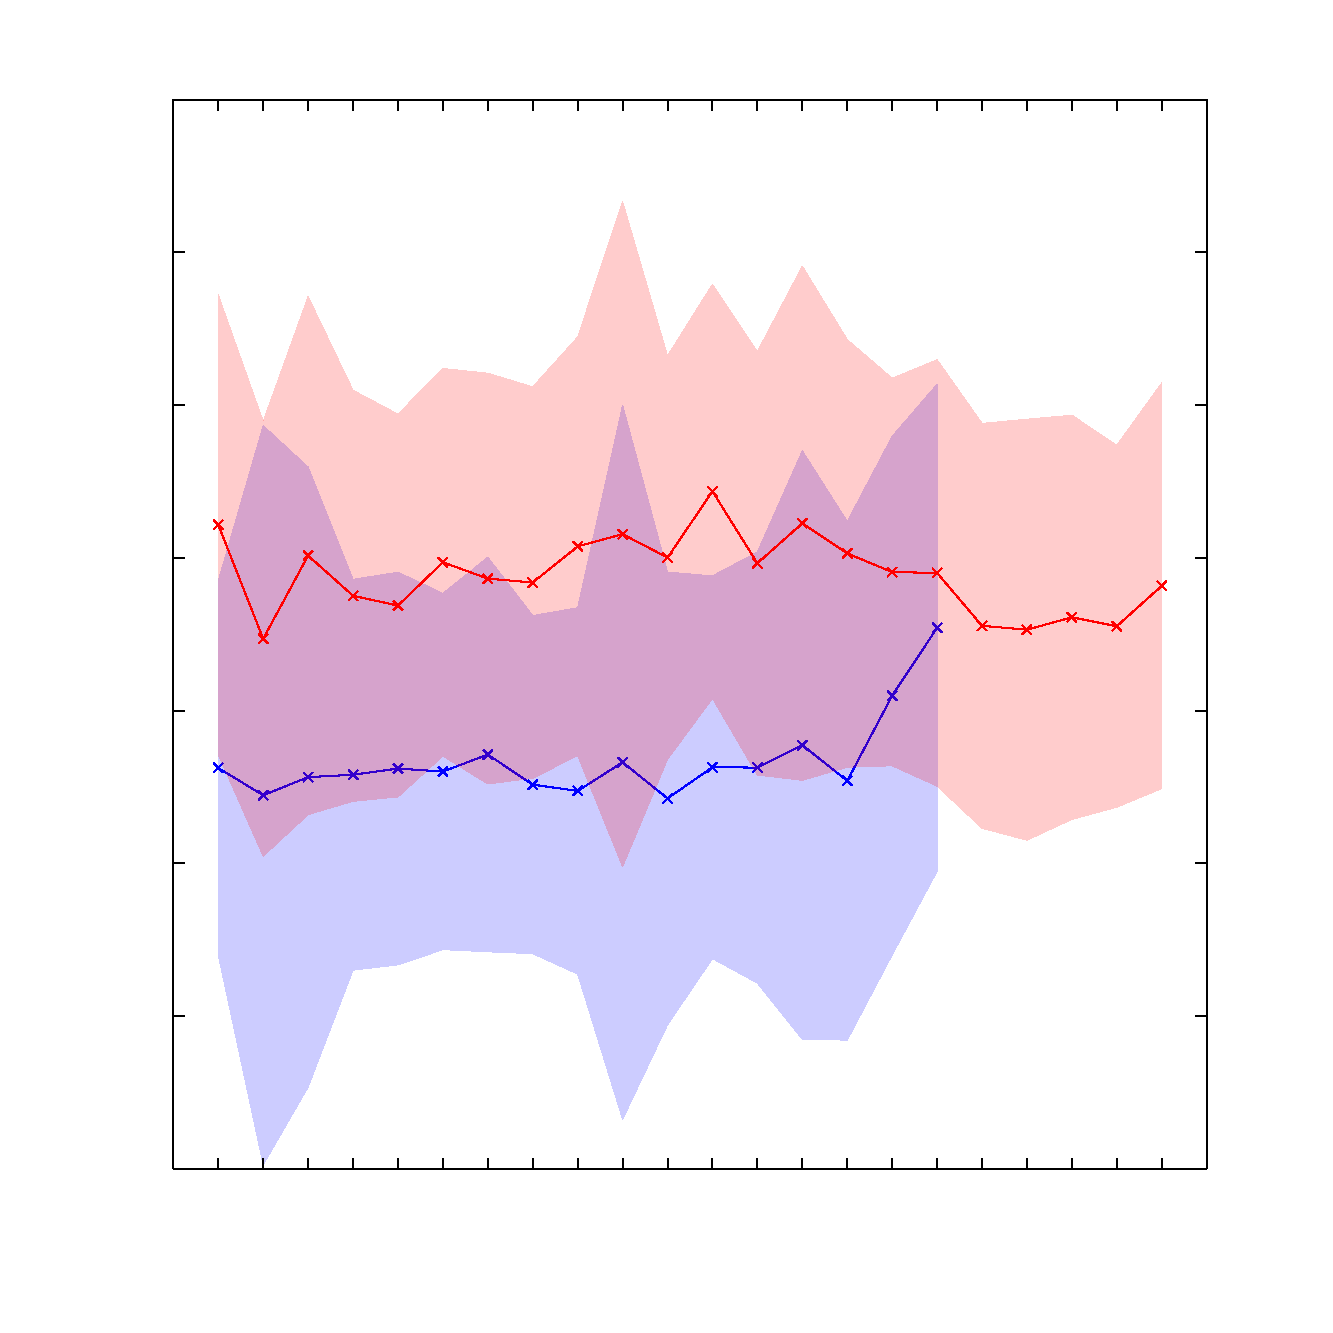
\includegraphics[width=0.47\linewidth]{figs/decoding/rcoef_sess_meanpc_v1_both.pdf}
% }
%     ~~
%     \subfloat[][\label{fig:noise_r_v4_all}\ac{V4}]{
% %         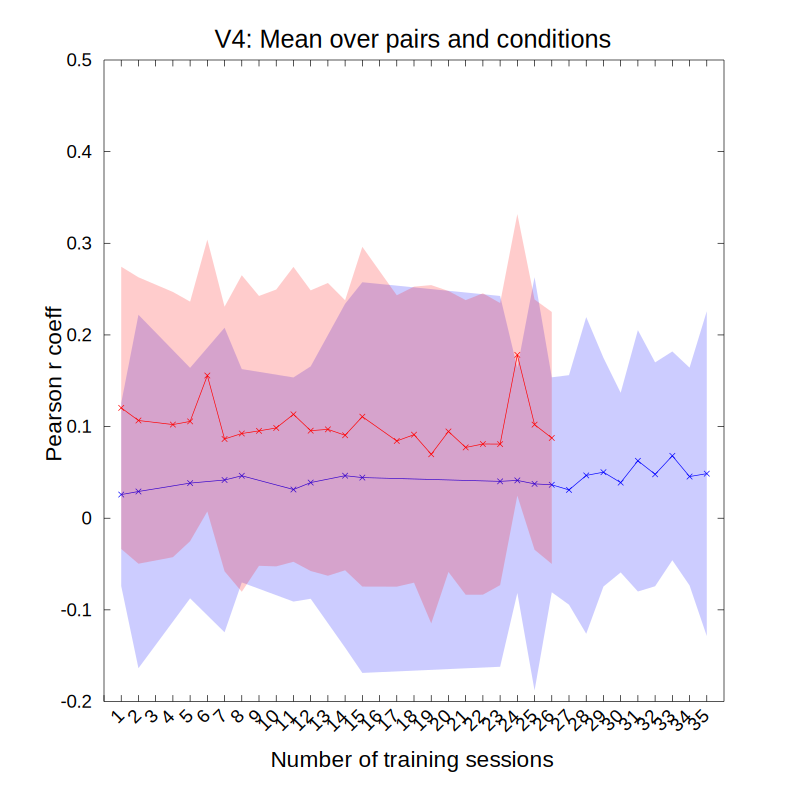
\includegraphics[width=0.47\linewidth]{%
% % ./rcoef_2013-04-09/rcoef_sess_meanpc_2013-04-09/png/rcoef_sess_meanpc_v4_both.png}
%         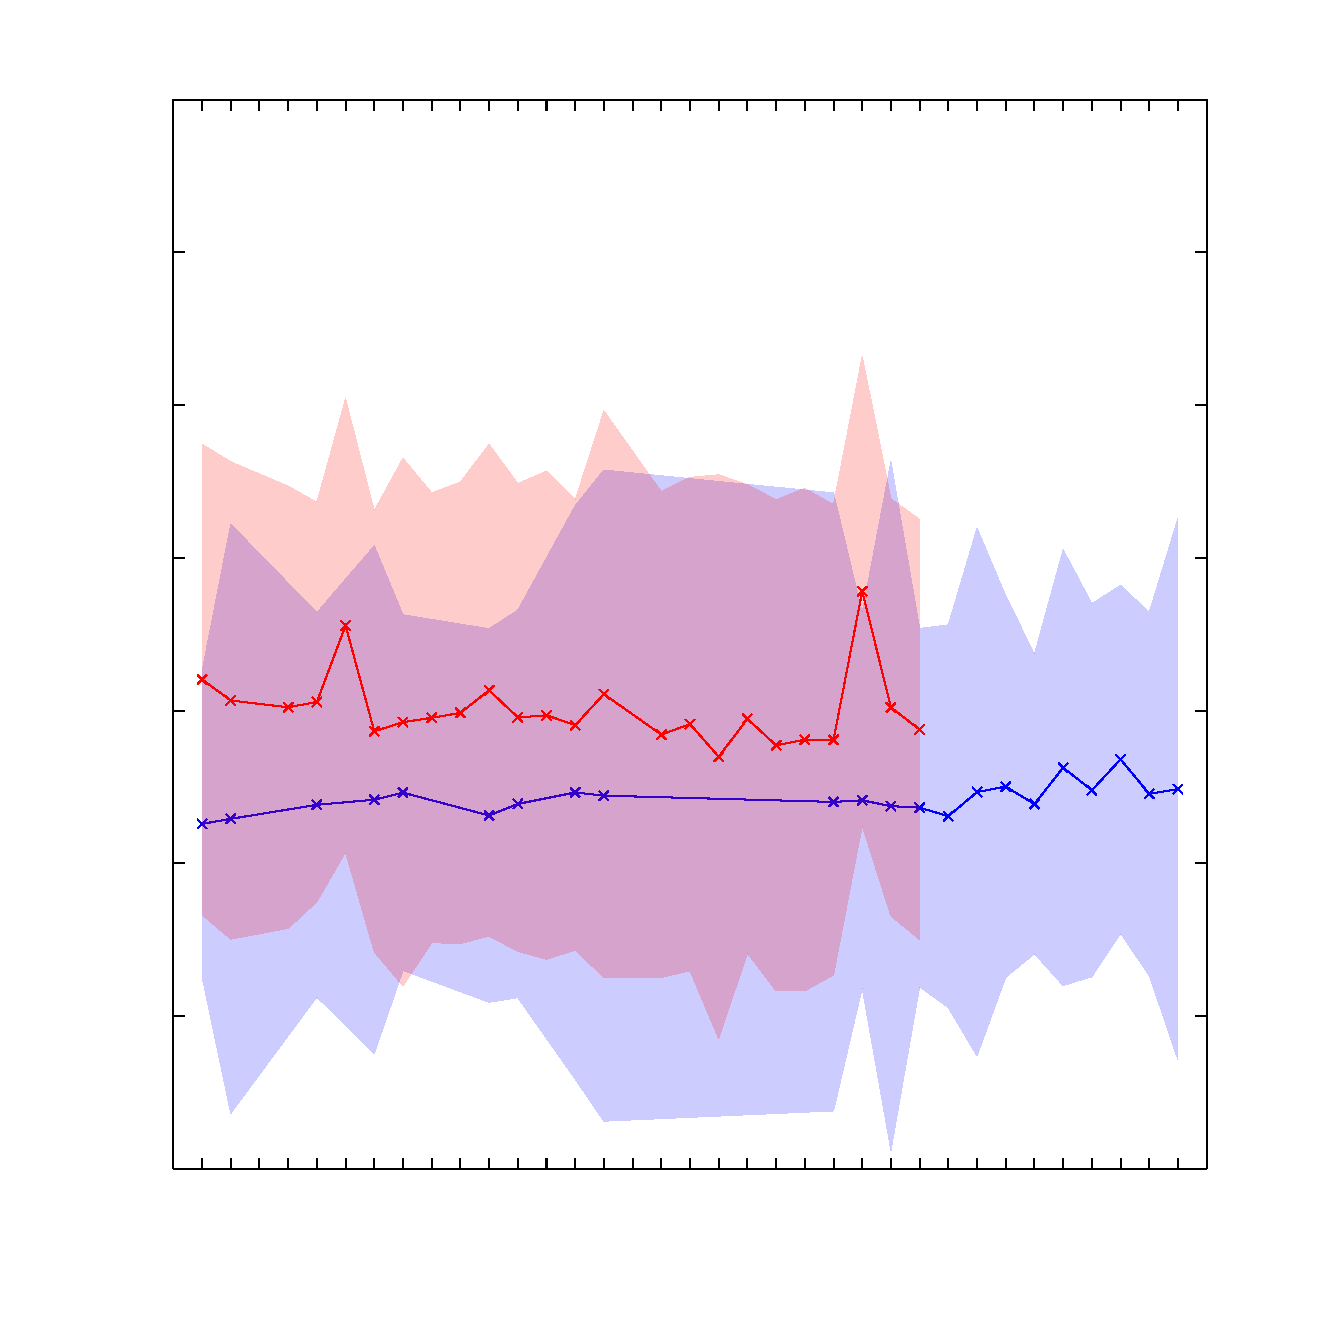
\includegraphics[width=0.47\linewidth]{figs/decoding/rcoef_sess_meanpc_v4_both.pdf}
% }
%     \caption{Change in noise correlations with learning.
% \protect\subref{fig:noise_r_v1_all}:~\ac{V1}.
% \protect\subref{fig:noise_r_v4_all}:~\ac{V4}.
% Blue:~\ac{M1}.
% Red:~\ac{M2}.
% On the x-axis, the number of sessions since the animal began training in the part of the visual field retinotopic to the recording site is shown.
% Line: pearson r coefficient, averaged across the possible pairings between channels for each of the 14 trial conditions.
% Shaded region indicates one standard deviation from mean.
% }
%     \label{fig:noise_r_all}
% \end{figure}
% % \marginnote{In \autoref{fig:noise_r_all} and \autoref{fig:noise_r_hist}, the text is too small due to saving the figure with transparencies in PNG format; if I could get the SVG to load correctly, the text would be sized correctly.}
%
% \autoref{fig:noise_r_hist} is intended to reproduce \citet[Figure 2C]{Gu2011}, with the distribution of $r$ shown across pairs for one pre-training and one post-training session.
% These sessions were chosen from a restricted set of sessions which did not have problems with artificially high correlations from the motion artifact, and selected from this set such that they were as close to the start and end of the training period as possible.
% However, this selection was made before the set of trials was redacted as mentioned in \autoref{sec:dec-meth-noise}, so the sessions selected could possibly be made further apart.
%
% The data presented in \autoref{fig:noise_r_hist} shows that the distribution of noise correlation pairs does not move significantly for \ac{M1} \ac{V1}, which is contrasted by a clear decrease for \ac{M2} \ac{V1}.
% It should be noted though that the distribution for \ac{M2} \ac{V1} begins higher than \ac{M1} and decreases to a similar value as \ac{M1} \ac{V1}.
% For \ac{V4}, there is an increase in mean noise correlation for \ac{M1} and a decrease for \ac{M2}, though as \ac{M2} begins higher than \ac{M1} the two do tend toward to one another.
%
% Cherry-picking is a significant problem here, as there is sizable day-to-day variation in the noise correlation across the pairs.
% Choosing a session where there is more noise correlation than neighbouring sessions at the beginning of training and less at the end of training will give the impression that there is a more significant decrease in noise correlations.
% More effort should be made to counter inadvertently cherry-picking in the session selection, as \autoref{fig:noise_r_j1_pmc} indicates this may be one reason for such a sizable decrease in noise correlation for \ac{M2} \ac{V1}.
%
% \begin{figure}[htbp]
%     \subfloat[][\label{fig:noise_r_b1_hist}]{
%         \centering
% %         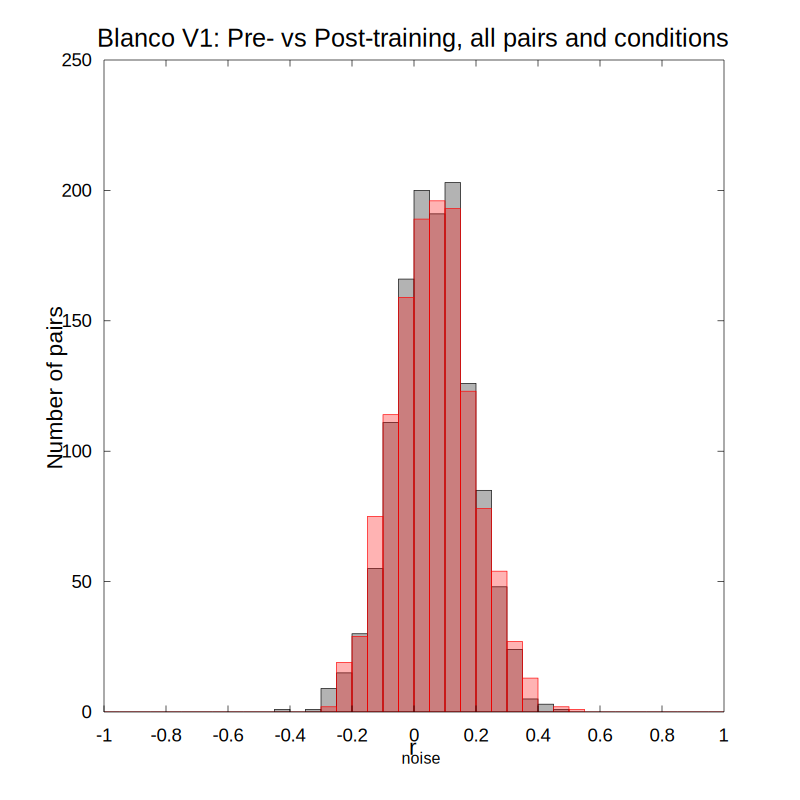
\includegraphics[width=0.47\linewidth]{%
% % ./rcoef_2013-03-25/rcoef_sess_histallover_2013-03-25/png/rcoef_sess_histallover_v1_blanco.png}
%         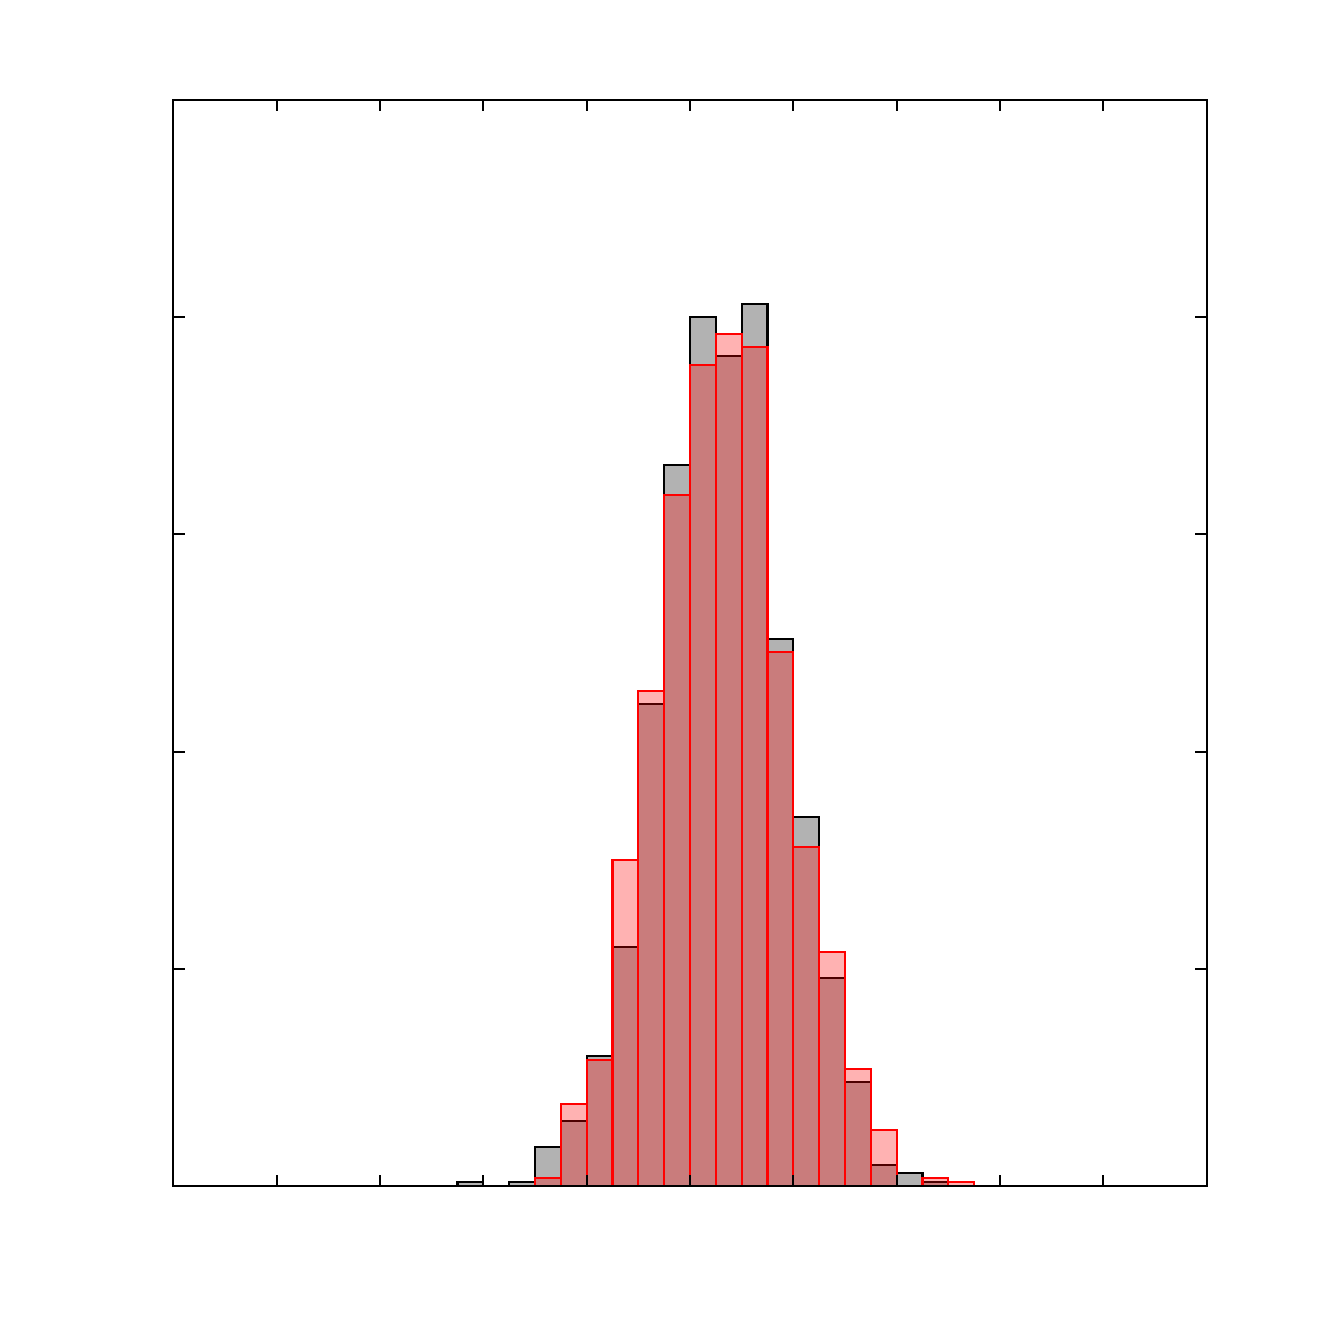
\includegraphics[width=0.47\linewidth]{figs/decoding/rcoef_sess_histallover_v1_blanco.pdf}
%     }
%     ~~
%     \subfloat[][\label{fig:noise_r_j1_hist}]{
%         \centering
% %         \includegraphics[width=0.47\linewidth]{%
% % ./rcoef_2013-03-25/rcoef_sess_histallover_2013-03-25/png/rcoef_sess_histallover_v1_jack.png}
%         \includegraphics[width=0.47\linewidth]{figs/decoding/rcoef_sess_histallover_v1_jack.pdf}
%     }
%     \\
%     \subfloat[][\label{fig:noise_r_b4_hist}]{
%         \centering
% %         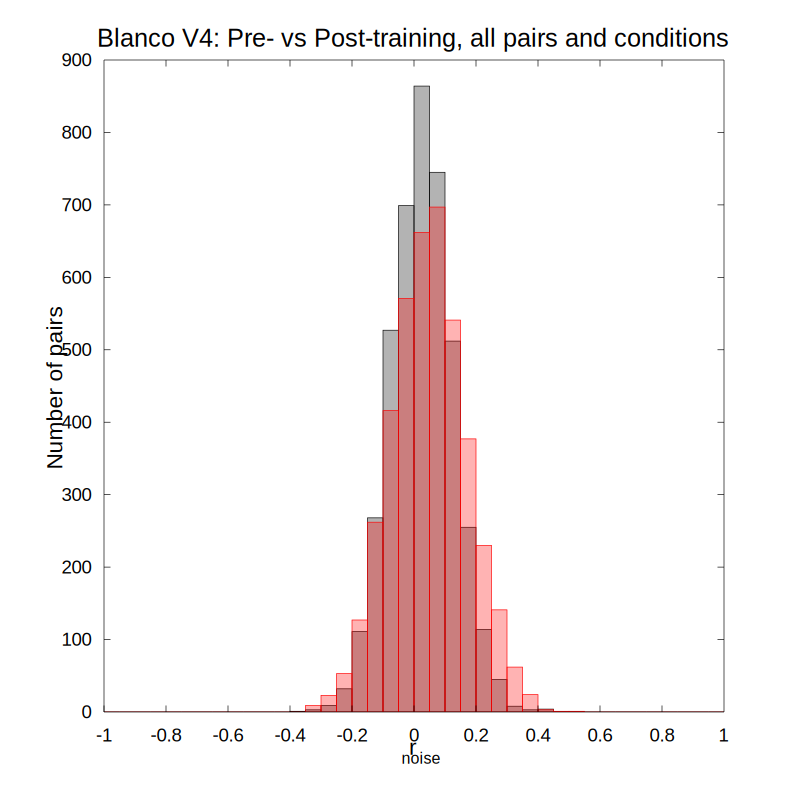
\includegraphics[width=0.47\linewidth]{%
% % ./rcoef_2013-03-25/rcoef_sess_histallover_2013-03-25/png/rcoef_sess_histallover_v4_blanco.png}
%         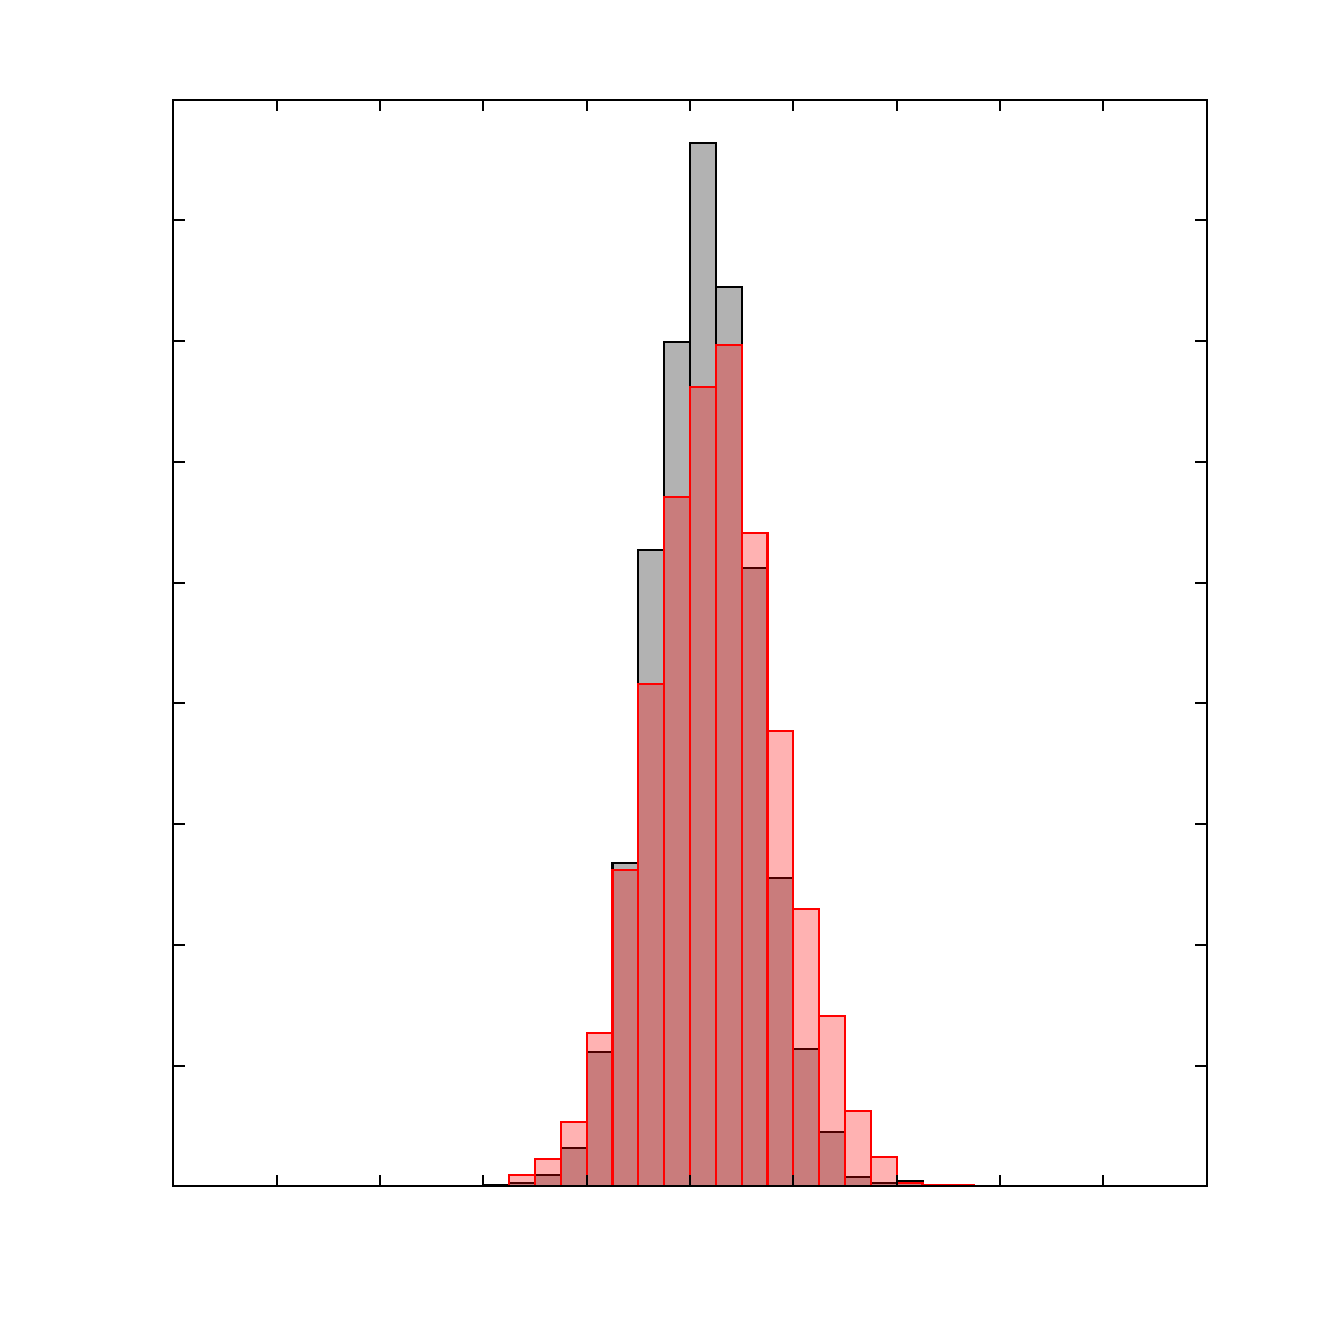
\includegraphics[width=0.47\linewidth]{figs/decoding/rcoef_sess_histallover_v4_blanco.pdf}
%     }
%     ~~
%     \subfloat[][\label{fig:noise_r_j4_hist}]{
%         \centering
% %         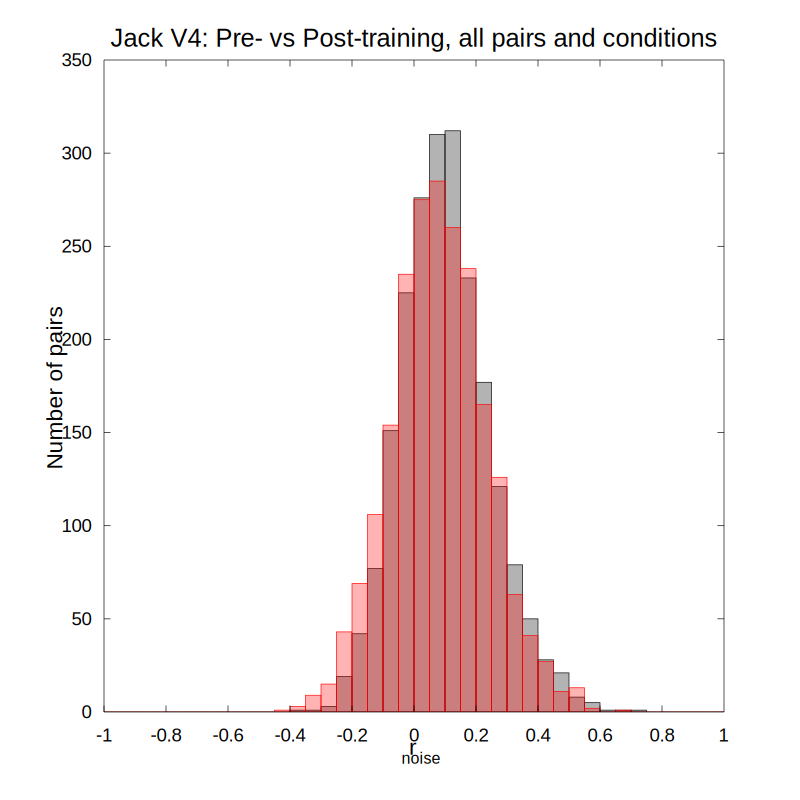
\includegraphics[width=0.47\linewidth]{%
% % ./rcoef_2013-03-25/rcoef_sess_histallover_2013-03-25/png/rcoef_sess_histallover_v4_jack.png}
%         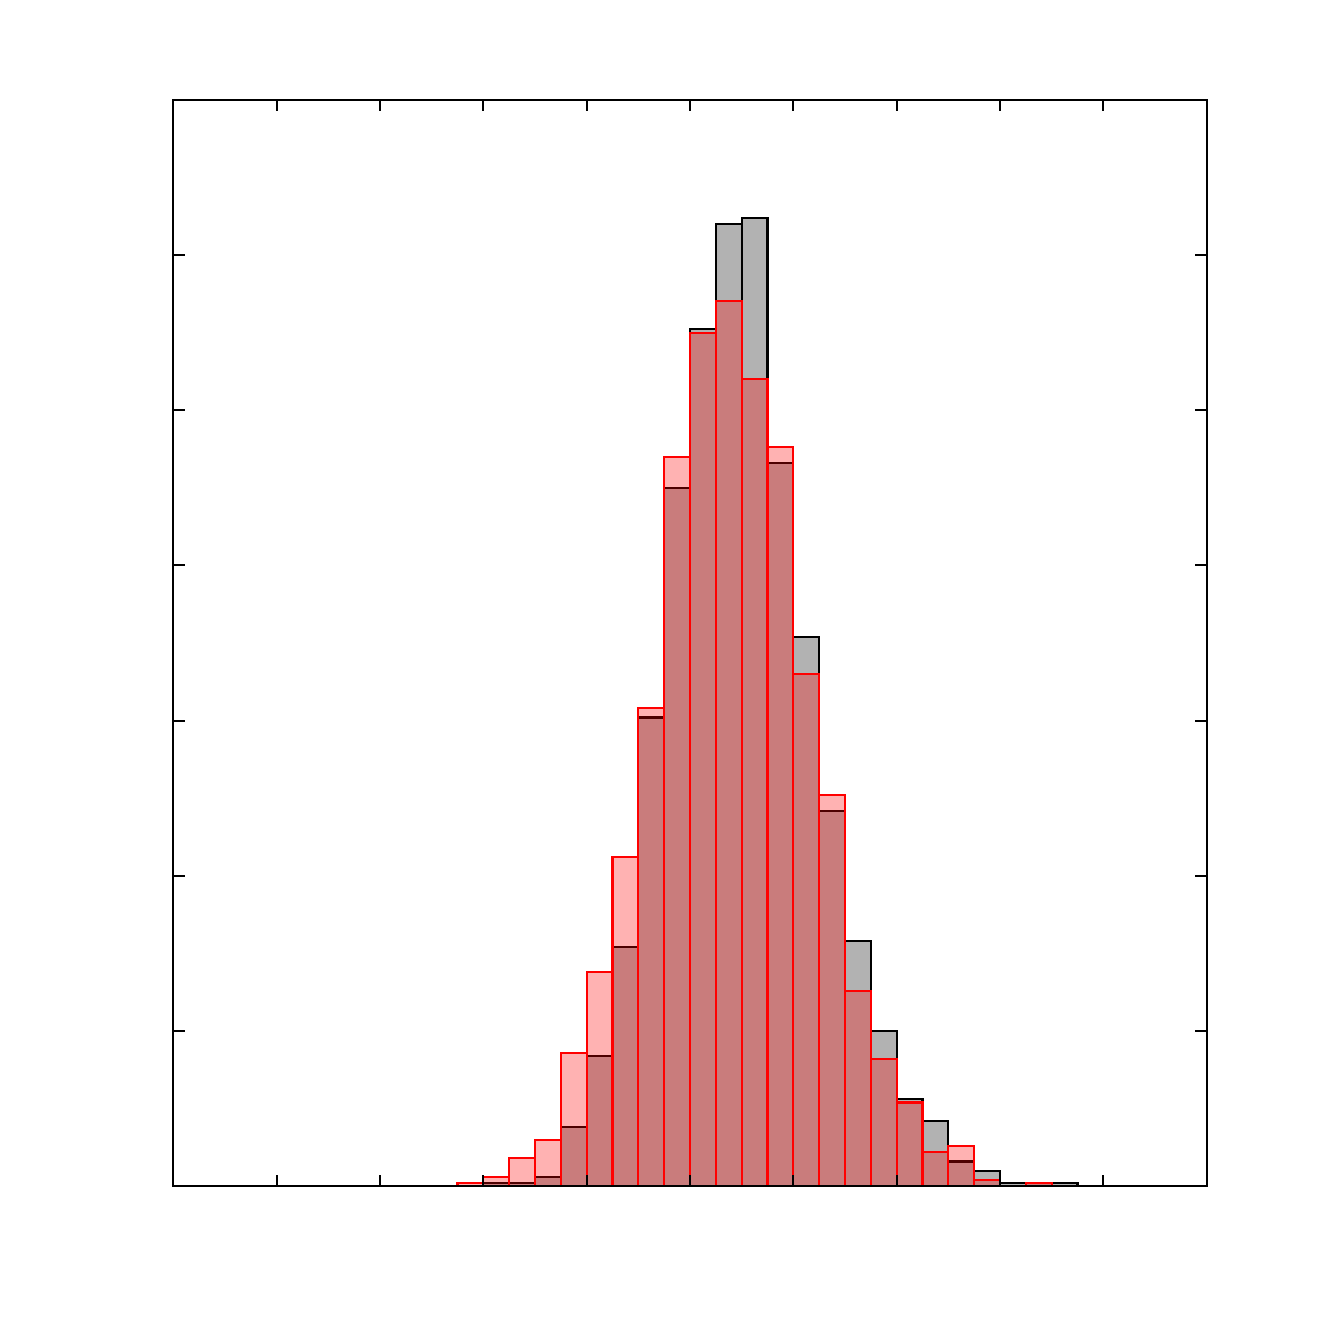
\includegraphics[width=0.47\linewidth]{figs/decoding/rcoef_sess_histallover_v4_jack.pdf}
%     }
%     \caption{Distribution of the noise correlations for the pairings across all conditions.
% Two sessions, one at the beginning of training (black) and one at the end of training (red) are shown for comparitive purposes.
% \protect\subref{fig:noise_r_b1_hist}: \ac{M1} \ac{V1}; sessions 343 and 354.
% \protect\subref{fig:noise_r_j1_hist}: \ac{M2} \ac{V1}; sessions 51 and 71.
% \protect\subref{fig:noise_r_b4_hist}: \ac{M1} \ac{V4}; sessions 307 and 338.
% \protect\subref{fig:noise_r_j4_hist}: \ac{M2} \ac{V4}; sessions 27 and 46.
% }
%     \label{fig:noise_r_hist}
% \end{figure}
%
%
% % \autoref{fig:noise_r_pmc} indicates that noise correlations are correlated for pairs across sessions.
% A pairs of channels which have higher noise correlations in one session are likely to have higher noise correlation in other sessions.
% However, this effect is not present for \ac{M1} \ac{V1}, \autoref{fig:noise_r_b1_pmc}, and could suggest there is less session-to-session consistency for this dataset.
%
% This figure provides an easy way of visually inspecting whether noise correlations are conserved, but does not allow us to quantify this.
%
% \begin{figure}[htbp]
%     \subfloat[][\label{fig:noise_r_b1_pmc}]{
%         \centering
%         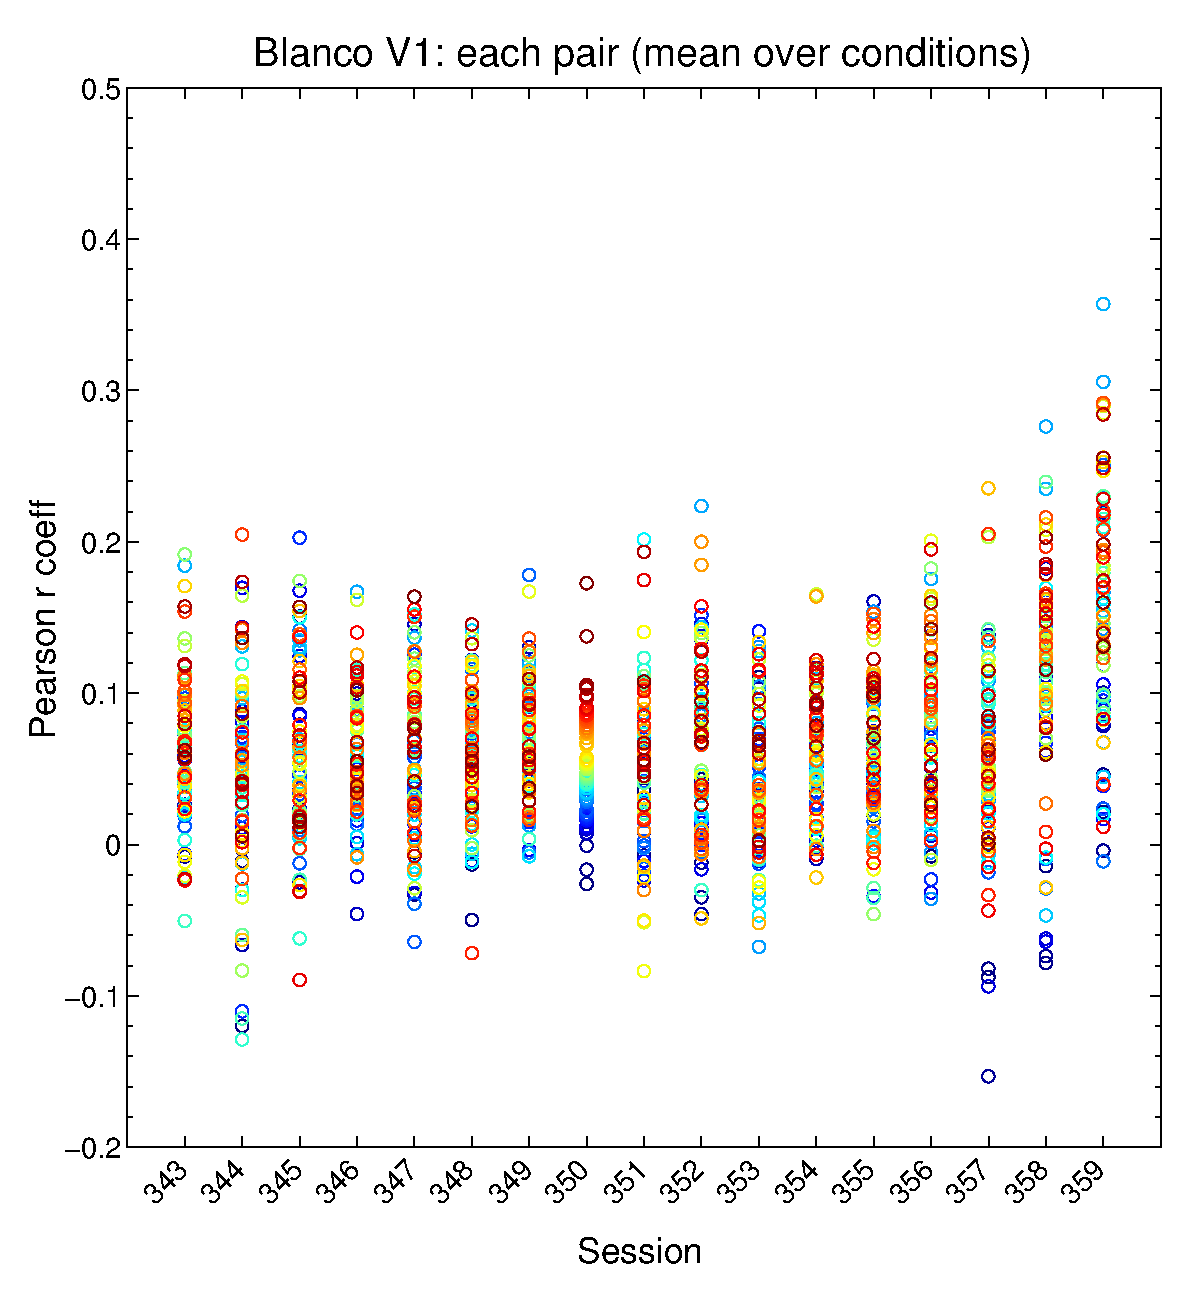
\includegraphics[width=0.47\linewidth]{%
% figs/decoding/rcoef_sess_pairsmeanc_v1_blanco.eps}
%     }
%     ~~
%     \subfloat[][\label{fig:noise_r_j1_pmc}]{
%         \centering
%         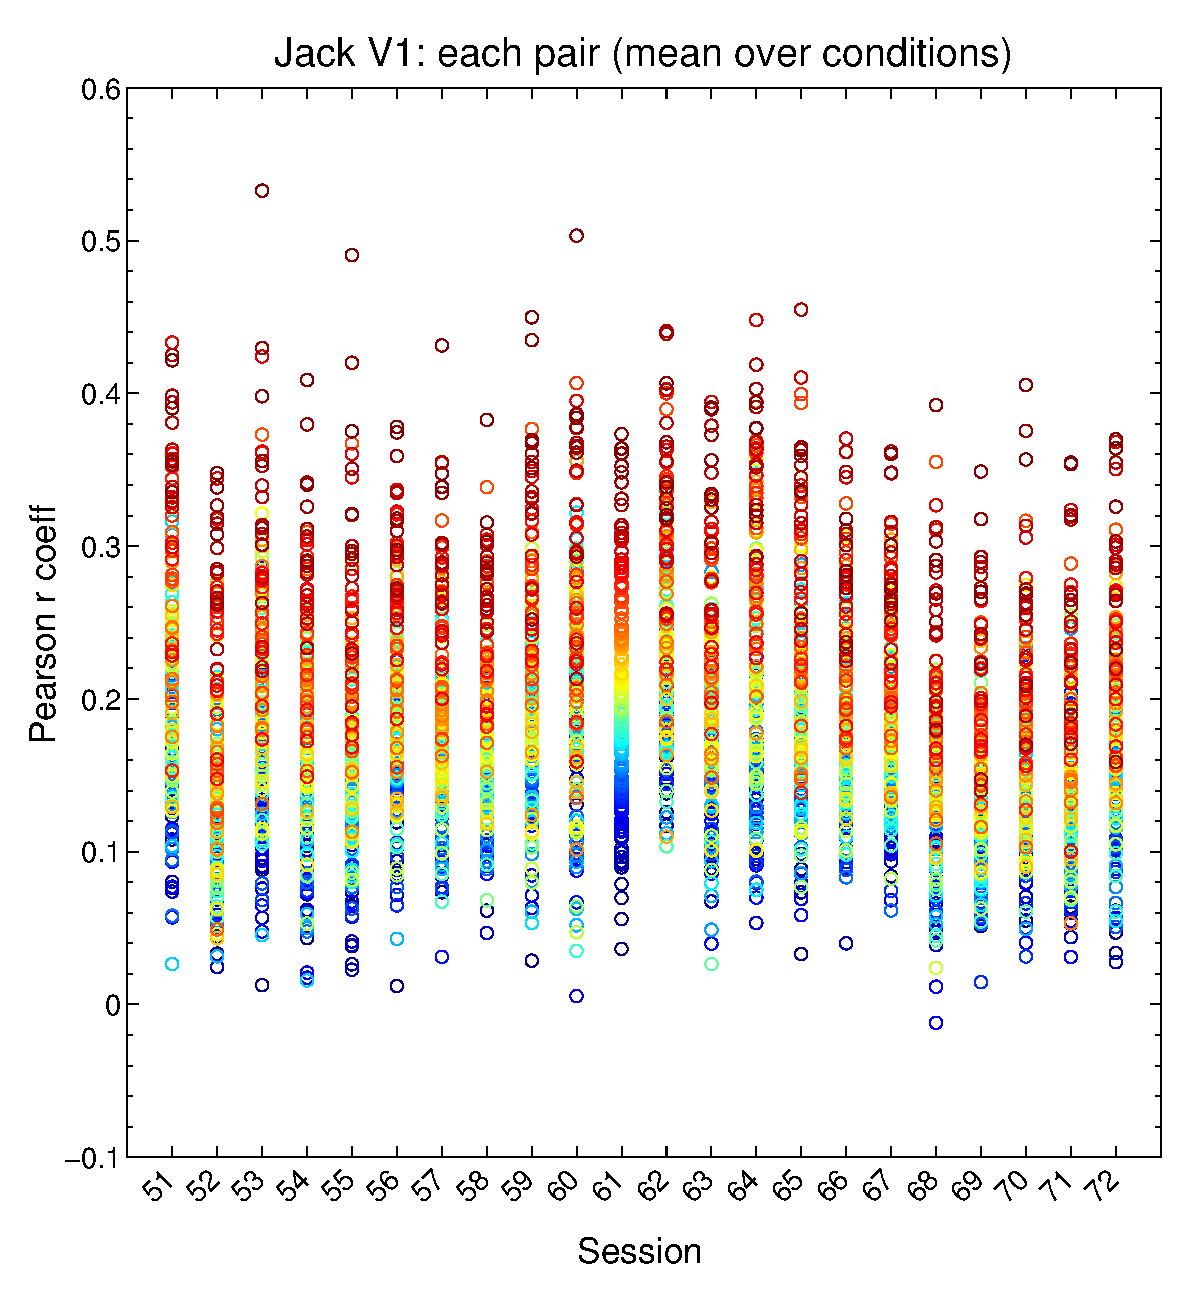
\includegraphics[width=0.47\linewidth]{%
% figs/decoding/rcoef_sess_pairsmeanc_v1_jack.eps}
%     }
%     \\
%     \subfloat[][\label{fig:noise_r_b4_pmc}]{
%         \centering
%         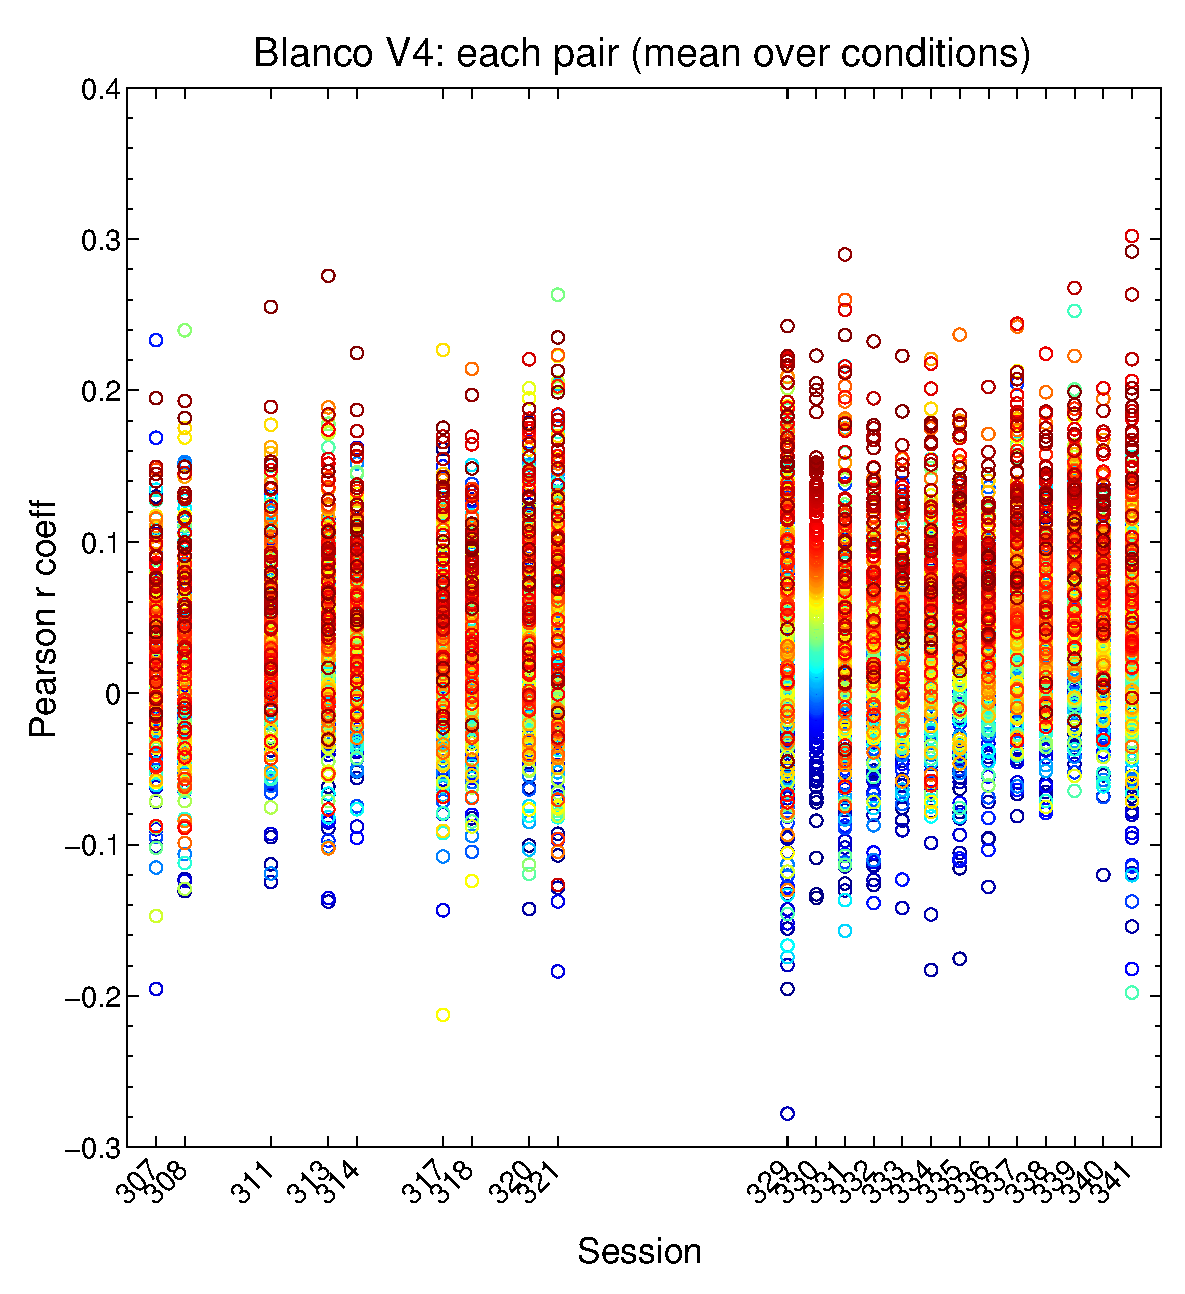
\includegraphics[width=0.47\linewidth]{%
% figs/decoding/rcoef_sess_pairsmeanc_v4_blanco.eps}
%     }
%     ~~
%     \subfloat[][\label{fig:noise_r_j4_pmc}]{
%         \centering
%         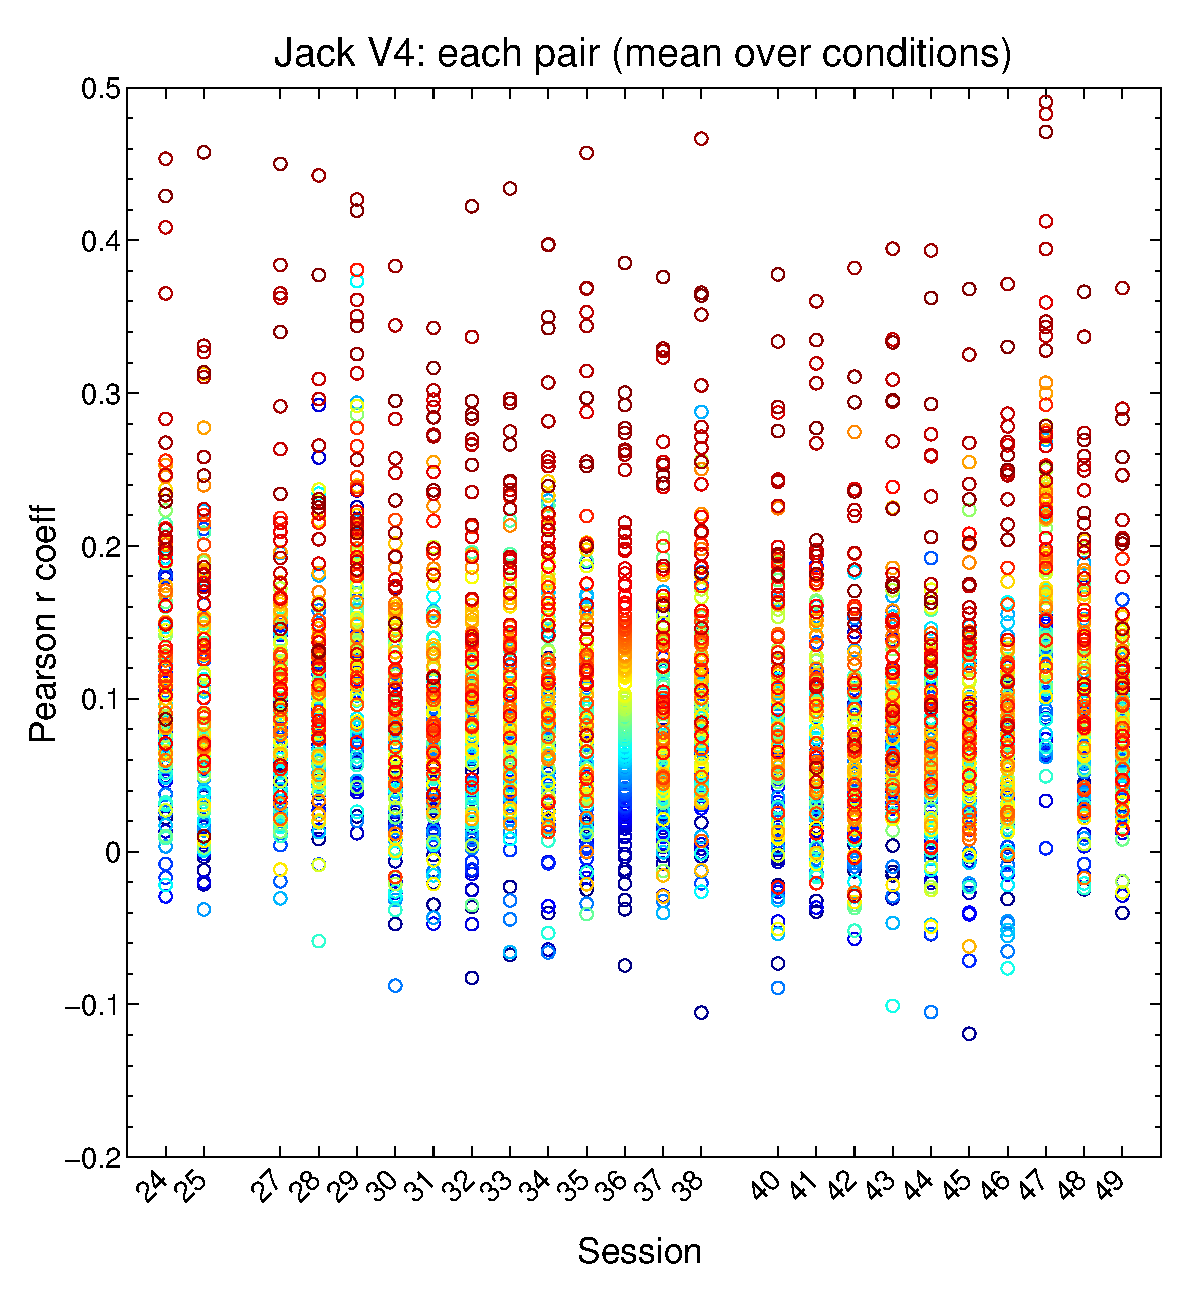
\includegraphics[width=0.47\linewidth]{%
% figs/decoding/rcoef_sess_pairsmeanc_v4_jack.eps}
%     }
%     \caption{Noise correlations for each pair, meaned across the 14 conditions.
% \protect\subref{fig:noise_r_b1_pmc}: \ac{M1} \ac{V1}.
% \protect\subref{fig:noise_r_j1_pmc}: \ac{M2} \ac{V1}.
% \protect\subref{fig:noise_r_b4_pmc}: \ac{M1} \ac{V4}.
% \protect\subref{fig:noise_r_j4_pmc}: \ac{M2} \ac{V4}.
% Colour is assigned by sorting the pairs into ascending order for one of the sessions near the middle of the training period.
% The degree of session-to-session correlation of the noise correlation can hence be inferred by visual inspection.
% }
%     \label{fig:noise_r_pmc}
% \end{figure}
%
%
%==============================================================================
\section{Sensitivity analysis}
\label{sec:pl_dprime}
%------------------------------------------------------------------------------

One simple method of comparing how the encoding of stimuli changes over time is to use the sensitivity index, $d'$.
This gives a measure of how separable the signal and the noise are, by comparing the difference in their means with the overall standard deviation.
% For a classifier, this is defined as the difference between the hit rate and the false alarm rate,
% \begin{equation}
% d' = P(A | A) - P(A | \bar{A})
% ,\end{equation}

For Gaussian distributed data, the sensitivity index is defined as
\begin{equation}
\label{eq:dprime}
d' = \frac{\mu_\text{stim} - \mu_\text{noise}}{\sigma_\text{joint}}
,\end{equation}
where the joint standard deviation is the root mean square of the standard deviation for each of two distributions,
\begin{equation}
% \sigma_\text{joint} = \sqrt
%     \frac{ (n_\text{stim}-1) \, \sigma_\text{stim}^2 + (n_\text{noise}-1) \, \sigma_\text{noise}^2 }
%     { n_\text{stim} + n_\text{noise} - 2}
\sigma_\text{joint} = \sqrt \frac{\sigma_\text{stim}^2 + \sigma_\text{noise}^2}{2}
.\end{equation}
For our analysis, the noise is the spiking activity during periods of spontaneous activity.
With the sample stimulus and 14 test stimuli with differing contrast levels, we have 15 possible signals to choose from for each dataset.
Since it has the most presentations and lies in the middle of the range of the contrasts, we will just consider $d'$ with respect to the response signal when presenting the sample stimulus.

The number of spikes over a finite duration, which cannot be negative, is typically Poisson distributed instead of Gaussian distributed.
However, the two distributions do converge for large $n$, and so we disregard this and use the Gaussian form of the definition of $d'$.

%------------------------------------------------------------------------------
\subsection{Methods for sensitivity analysis}
\label{sec:violin_plot_method}

To compute $d'$, we used the number of spikes occurring during a \SI{1050}{\milli\second} period of activity.
The spontaneous (noise) activity was defined as the number of spikes detected during the \SI{525}{\milli\second} immediately preceding the sample stimulus onset.
The signal activity was the number of spikes during the \SI{525}{\milli\second} immediately following the sample stimulus onset.
From this, $d'$ was computed using \autoref{eq:dprime}.

To investigate whether $d'$ changed significantly during the course of our experiments, we compared the average $d'$ during the first and final three experimental sessions (\zonename{A} and \zonename{B}).
A paired $t$-test (two-tailed) was used to study whether the $d'$ consistently increased or decreased for the channels.

The violin plots (see, for instance, the upper-right panel of \autoref{fig:dprime_v1_blanco}) show the Gaussian kernel density estimation of the distribution over channels of $d'$ before and after training (\zonename{A} and \zonename{B}).
This bandwidth of the Gaussian kernel was determined using the rule of thumb bandwidth estimator,
\begin{equation}
h = \hat{\sigma} \left( \frac{4}{3 n} \right) ^ \frac{1}{5}
,\label{eq:estimate-bw}\end{equation}
where $n$ is the number of samples and $\hat{\sigma}$ is the estimated standard deviation for the population determined from these samples.
We applied the bandwidth estimator to the set of $d'$ averaged over the first three sessions of training, $\SET{\zonename{A}}$, and averaged over final three sessions, $\SET{\zonename{A}}$, to find $h_\zonename{A}$ and $h_\zonename{B}$.
In each plot, the same kernel bandwidth of
$H = \min(h_\zonename{A}, h_\zonename{B}) / 2$
is used when estimating the density at \zonename{A} and at \zonename{B}.
This ensures sufficient detail about the distribution is preserved for each, and the two are comparable with each other.

%------------------------------------------------------------------------------
\subsection{Results for \acs{V1} sensitivity}

% blanco v1
% same bandwidth bw = 0.26027 used for all cols
% h=1.000000 p=0.021169=2.116899e-02 delta=-0.322850
% jack v1
% same bandwidth bw = 0.21865 used for all cols
% h=1.000000 p=0.000000=3.274440e-07 delta=-0.418598

For \ac{V1}, we found the $d'$ decreased with training (see \autoref{fig:dprime_v1}).
A similar result was observed for each subject.
The average change in was $\Delta d' = -0.323$ ($p=0.02$, paired $t$-test) for \ac{M1} and $\Delta d' = -0.419$ ($p < 4 \times 10 ^{-7}$, paired $t$-test) for \ac{M2}.
 
\begin{figure}[htbp]
    \centering
    \hspace*{\fill}
    \subfloat[\ac{M1} \ac{V1}\label{fig:dprime_v1_blanco}]{
        \centering
        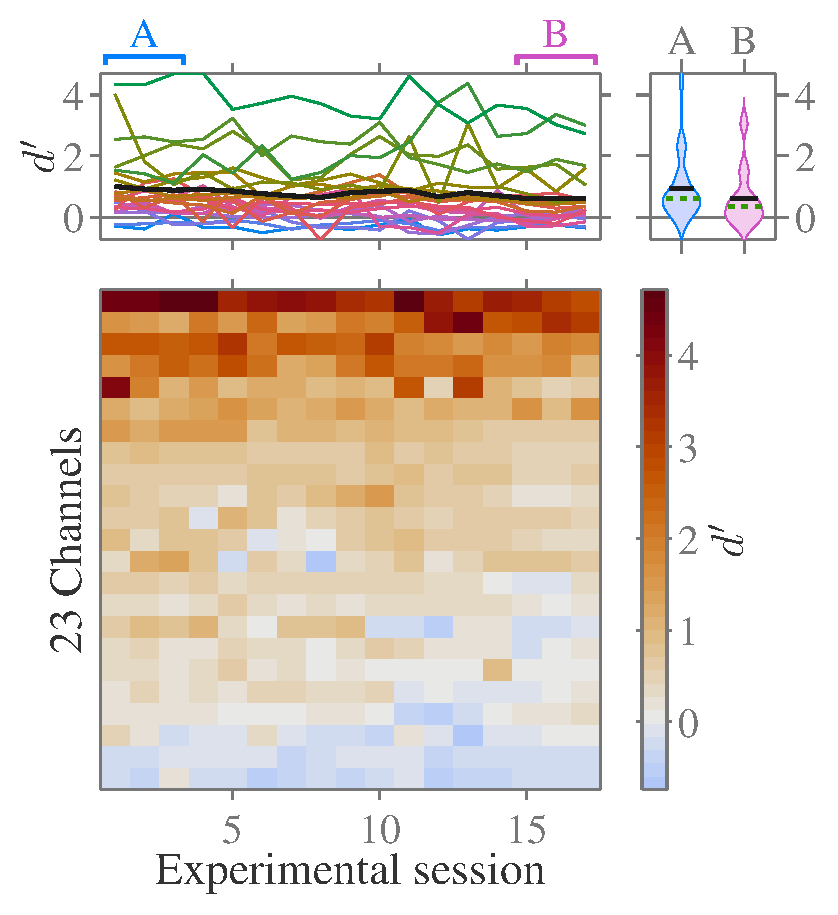
\includegraphics[scale=.45]{%
figs/dprime/dprime_sample_hm_hotcold_blanco_v1_1_rmon2_rmvet2.eps}
    }
    \hspace*{\fill}\hspace{.2cm}\hspace*{\fill}
    \subfloat[\ac{M2} \ac{V1}\label{fig:dprime_v1_jack}]{
        \centering
        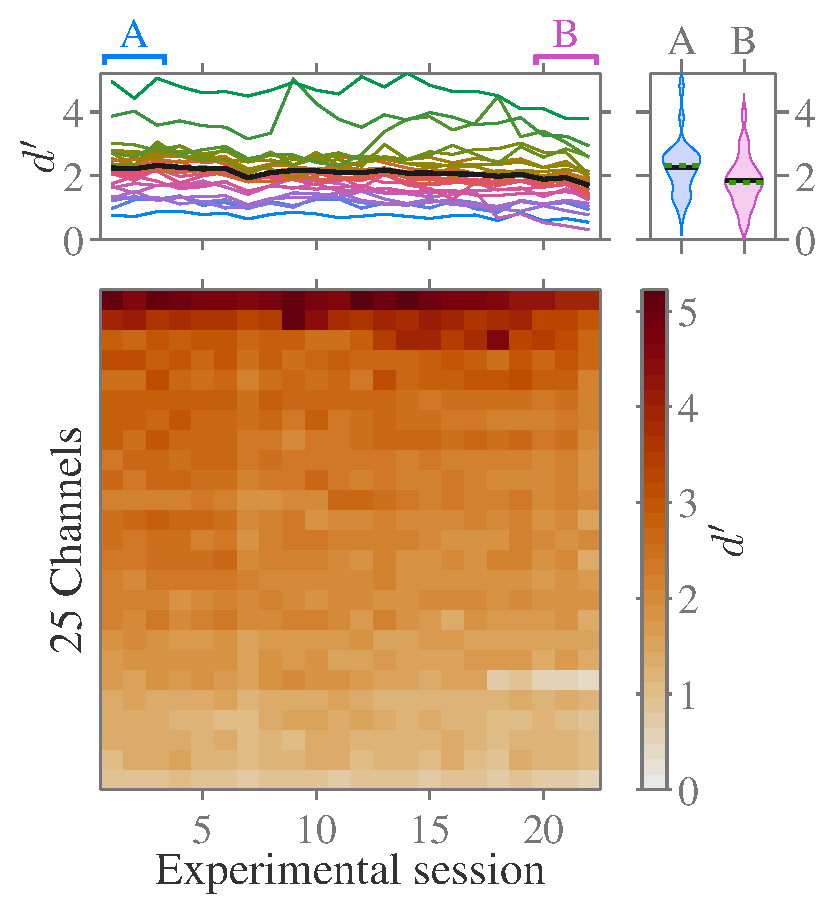
\includegraphics[scale=.45]{%
figs/dprime/dprime_sample_hm_hotcold_jack_v1_1_rmon2_rmvet2.eps}
    }
    \hspace*{\fill}
    \caption{Change in $d'$ over training sessions for \ac{V1} recordings.
\protect\subref{fig:dprime_v1_blanco}: $d'$ for \ac{M1}, shown for each recording channel, with channels ordered according to average $d'$ over all sessions.
Above, traces of $d'$ for each channel (colours), and average over channels (black).
Below, heatmap showing $d'$ for each channel.
Right top, violin plots showing distribution over channels of the average $d'$ in the first three sessions (\zonename{A}) and last three sessions (\zonename{B}), with mean (solid black line) and median (dashed green line) over channels indicated.
The violin plot shows a Gaussian kernel density using a bandwidth determined automatically as described in \autoref{sec:info-methods}.
\protect\subref{fig:dprime_v1_jack}: Same as \protect\subref{fig:dprime_v1_blanco}, but for \ac{M2}.
}
    \label{fig:dprime_v1}
\end{figure}


\subsection{Results for \acs{V4} sensitivity}
\label{sec:pl_dprime_v4}

% blanco v4
% same bandwidth bw = 0.17898 used for all cols
% h=0.000000 p=0.463346=4.633457e-01 delta=+0.052346
% jack v4
% same bandwidth bw = 0.064737 used for all cols
% h=1.000000 p=0.000000=6.946514e-08 delta=+0.491173

The results for \ac{V1} contrast with our findings for \ac{V4}.
For \ac{M1}, some channels marginally increased and others marginally decreased their $d'$ with training (\autoref{fig:dprime_v4_blanco}).
Overall, there was a small increase in average $d'$, with $\Delta d' = +0.052$, which was not a statistically significant change ($p=0.46$).

With \ac{M2}, many channels began training either indifferent to the stimulus, $d'=0$, or were suppressed by it, $d'<0$ (\autoref{fig:dprime_v4_jack}).
Starting from this lower position, there was a significant increase of $\Delta d' = +0.491$ ($p < 7 \times 10 ^{-8}$).
However the final $d'$ for almost all channels recorded for \ac{M2} was still lower than the average $d'$ for \ac{M1}.

\begin{figure}[htbp]
    \centering
    \hspace*{\fill}
    \subfloat[\ac{M1} \ac{V4}\label{fig:dprime_v4_blanco}]{
        \centering
        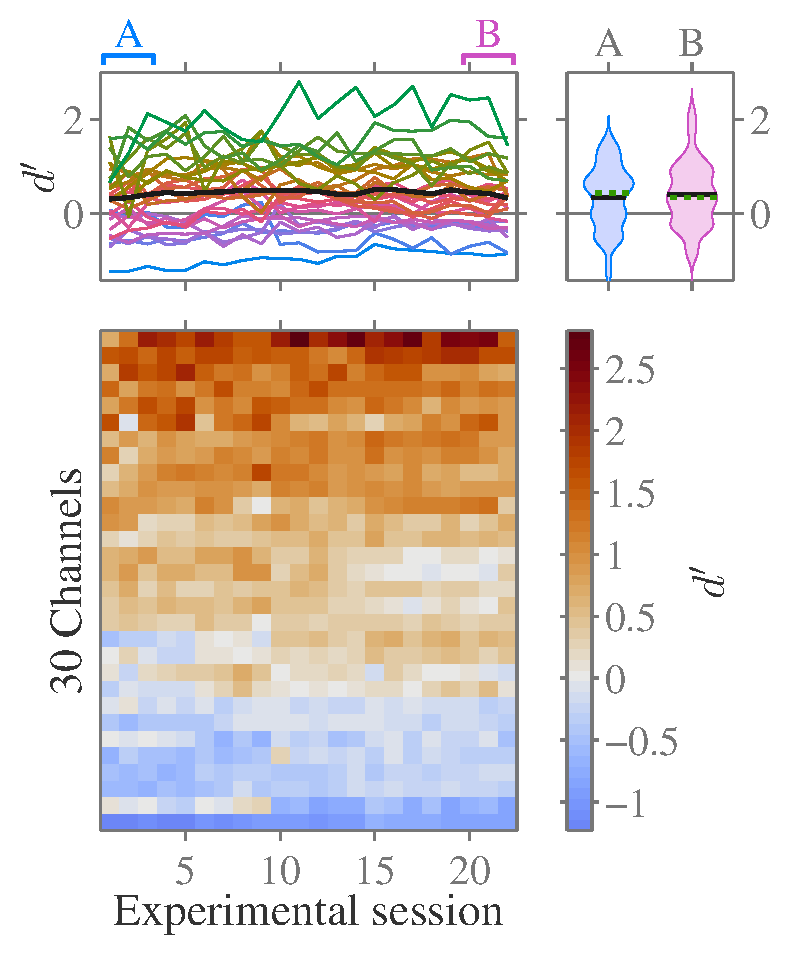
\includegraphics[scale=.45]{%
figs/dprime/dprime_sample_hm_hotcold_blanco_v4_1_rmon2_rmvet2.eps}
    }
    \hspace*{\fill}\hspace{.2cm}\hspace*{\fill}
    \subfloat[\ac{M2} \ac{V4}\label{fig:dprime_v4_jack}]{
        \centering
        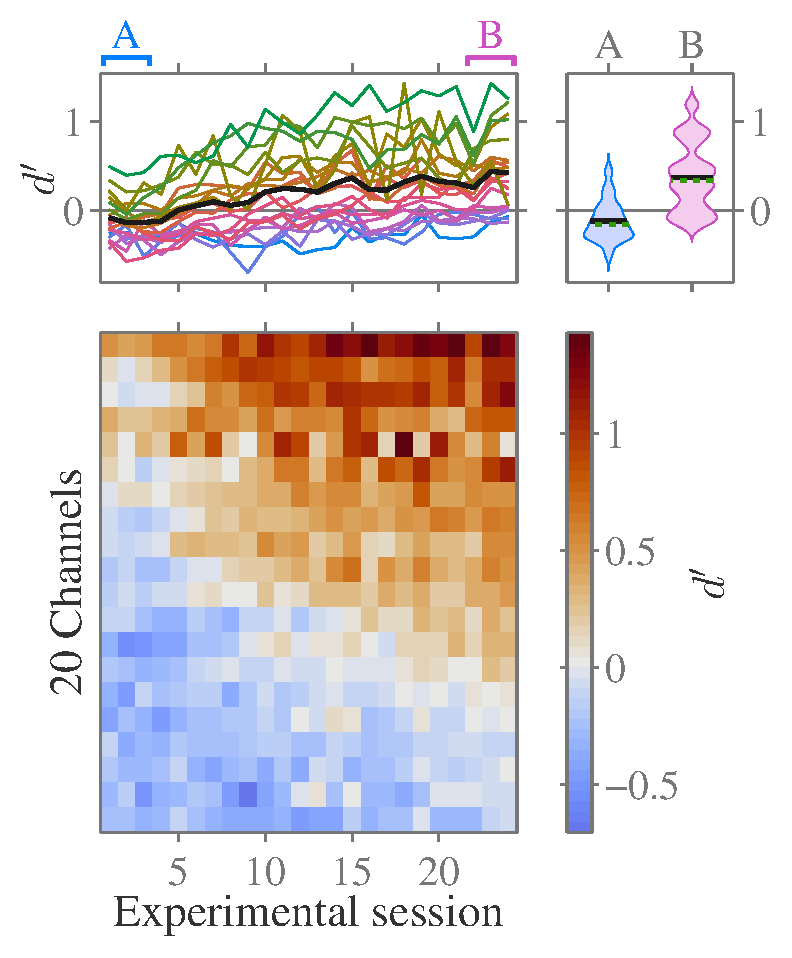
\includegraphics[scale=.45]{%
figs/dprime/dprime_sample_hm_hotcold_jack_v4_1_rmon2_rmvet2.eps}
    }
    \hspace*{\fill}
    \caption{Same as \autoref{fig:dprime_v1}, but for $d'$ during \ac{V4} recordings.
\protect\subref{fig:dprime_v4_blanco}: \ac{M1}.
\protect\subref{fig:dprime_v4_jack}: \ac{M2}.
}
    \label{fig:dprime_v4}
\end{figure}


\subsection{Discussion of sensitivity}
\label{sec:pl_dprime_discuss}

By analysing the sensitivity index, $d'$, we can see whether channels become more or less responsive to our stimulus class over time.
Since \ac{V1} is an early step in the visual processing hierarchy, its neurons respond strongly to simple stimuli such as the sinusoidal gratings we present.
Consequently, neurons have large responses to our stimuli even from the first session of the experimental training.
Over time, we found a decrease in sensitivity in \ac{V1} for both subjects.
We suspect this decrease in sensitivity of the neural response in \ac{V1} to the sample stimulus is due to unpreventable deterioration in the recording quality of the implanted chronic electrodes over time.
Over time, the noise increases and the signal-to-noise ratio falls, which leads to a reduction in the distinguishability of the two activity distributions.

On the other hand, \ac{V4} is higher up the visual hierarchy and in general responds to more a complex stimulus class.
For \ac{M1}, many of the neurons we recorded from were responsive to the primitive Gabor stimulus from the beginning of training.
But for \ac{M2}, this was not the case --- on the contrary, many neurons were suppressed by the Gabor stimulus.
With training, neurons recorded in \ac{M1} did not notably change their sensitivity to the sample stimulus, whereas $d'$ did increase for \ac{M2}.

We make particular note of the fact that the $d'$ in \ac{V4} increased for \ac{M2} from mostly negative initially values.
In principle, a decrease in activity in response to a stimulus can provide as much information about the presence of the stimulus as increase in activity.
However, it is difficult for neurons to increase their spontaneous activity due to the constraining effects of homeostasis, and it would be energetically inefficient for them to do so.
Therefore, since the firing rate of a neuron cannot fall below $0$ there is a smaller limit to the amount by which firing rates can differ if the information about the stimulus is conveyed by a reduction in activity compared to the background rate.
To provided more sensitivity for the response to our experimental stimuli, it thus makes sense for neurons which are suppressed by the stimulus class to increase their responses such that they are enhanced by its presence.
In practice, the de-suppression of the responses may arise not from the need of many individual neurons to encode the stimulus, but from a small number increasing the magnitude of their responses and then the connected neurons (which are positively correlated) increase their responses also.

From these results, we hypothesise that the sensitivity of the response to the experimental stimuli increases for the local network retinotopic to the stimulus location if it is too low for the network overall.
If the neurons are sufficiently sensitive to the stimulus to begin with (if $d'$ is high enough) then the sensitivity remains the same and does not increase with training.
Of course, the recorded sensitivity may decrease due to the decline in the recording quality.

With this measure, we can determine which channels contain neurons which change their relative responsiveness to the stimulus class, but we do not know how the distribution of responses change across the 14 different stimuli.
It is certainly plausible for neurons which begin their training already responsive to the stimuli to change their distribution of activity with respect to the contrast of the stimulus to provide more pertinent information for the experimental task.
For instance, this would be achieved if the absolute activity in response to the sample stimulus remains the same but the rate of change of activity with respect to the contrast of the stimulus increases.


%==============================================================================
\FloatBarrier
\section{Information in individual channels}
%------------------------------------------------------------------------------

We now apply the principles of Shannon information, as described in \autoref{sec:bgit}, to the perceptual learning data.
We are interested in how easy it is to determine which contrast the stimulus was presented with by observing the neural activity in response to the stimulus.
Since the subject's performance increases with training, we expect to find the amount of information encoded in the neural activity to increase with training.
This much is trivial, since perception occurs within the neural activity of an individual.
What will be interesting to uncover is \textit{where} the neural changes take place --- in \ac{V1}, in \ac{V4}, neither, or both?

To make its decision, the subject has access to all the neurons we have recorded and all the neurons in the brain from which we have not recorded.
Consequently, it would for the best idea of how much information the brain has access to, we would evaluate how much information is contained in the vector of neuronal responses for every recording channel.
However, this is problematic.
As the number of data streams combined into the response vector increases, the number of possible unique response vectors increases exponentially.
However, the number of trials recorded is fixed, and the number of possible response vectors must be constrained to prevent the estimated amount of information diverging to infinity (see \autoref{sec:bgit}).

Therefore, in this section we consider the information about the contrast of the stimulus encoded in the firing rate detected from only a single channel at once.
In doing so, we will ignore the possible redundancy or synergy in the information encoded by the response of multiple channels.
Later, in \autoref{sec:dec-meth-lin}, we will consider the total information encoded in the population response.
It should be noted that, since the spikes detected from each channel have been left unsorted and not resolved into clusters corresponding to individual neurons, this will be a multi-unit analysis, but only in the sense of neighbouring neurons being detected by the same electrode contact.


%------------------------------------------------------------------------------
\subsection{Methods for computing information}
\label{sec:info-methods}

The mutual information between the spiking activity during the presentation of the test stimulus and the identity of that stimulus was computed using the \textit{Information Breakdown Toolbox} for MATLAB \citep{Magri2009}.
Bias correction was performed using the \ac{PT} method (see \autoref{sec:bgit}) unless indicated otherwise.

To test the significance of changes in information over time, we used a paired Student's $t$-test to compare the difference in information values in $\SET{\zonename{A}}$ and $\SET{\zonename{B}}$ against the null-hypothesis of no change between points \zonename{A} and \zonename{B}.
Although the distribution of information values is evidently non-Gaussian (it is bounded below at \SI{0}{bits}), the distribution in differences in information is close to Gaussian.
We could instead have used the Mann--Whitney $U$ test to compare the two distributions $\SET{\zonename{A}}$ and $\SET{\zonename{B}}$.
This test does not assume the two distributions are Gaussian, but makes the additional assumption that all samples are independent.
Since we record from the same set of channels for both $\SET{\zonename{A}}$ and $\SET{\zonename{B}}$, we are violating the independence assumption, and so the paired Student's $t$-test is a more appropriate choice.

We show the Gaussian kernel estimation of the distribution of information over channels (a ``violin plot'', right-hand panel of \autoref{fig:info_sess_1x527_v1_blanco}, for instance) at the start (\zonename{A}) and end (\zonename{B}) of training.
These were found using the same method as described in \autoref{sec:violin_plot_method}.
Again, the kernel bandwidth was selected as
$H = \min(h_\zonename{A}, h_\zonename{B}) / 2$
to ensure sufficient detail was captured and the two density estimates are comparable.


%------------------------------------------------------------------------------
\subsection{Initial analysis}
\label{sec:pl_initial}

First, we will consider the amount of information about the stimulus contained in a simple firing rate encoding.
For each test stimulus presentation, our response is the total number of spikes which were detected from a single channel during the first \SI{527}{\milli\second} of the stimulus presentation.%
\footnote{This duration is chosen because there is slight variation in the stimulus presentation time, and \SI{527}{\milli\second} is the shortest presentation duration.}

For each recording channel, we computed how much information was contained in this overall firing response about the identity of which stimulus had been presented.
The results of this initial analysis are shown in \autoref{fig:info_sess_1x527}.
We found that information in the overall firing rate of \ac{V1} channels increased with training for \ac{M2} (\SI{+0.069\pm0.017}{bits} or \SI{+16\pm5}{\percent} relative change, $p=0.0004$) but not for \ac{M1} (\SI{-0.051\pm0.029}{bits} or \SI{-34\pm19}{\percent}, $p=0.09$).
For \ac{V4}, there was an increase in information for both subjects however this increase was significant for \ac{M2} (\SI{+0.056\pm0.013}{bits} or \SI{+87\pm21}{\percent}, $p=0.0005$) but not \ac{M1} (\SI{+0.028\pm0.020}{bits} or \SI{+22\pm16}{\percent}, $p=0.17$).


\begin{figure}[htbp]%
    \centering
    \hspace*{\fill}
    \subfloat[][\ac{M1} \ac{V1}.\label{fig:info_sess_1x527_v1_blanco}]{%
        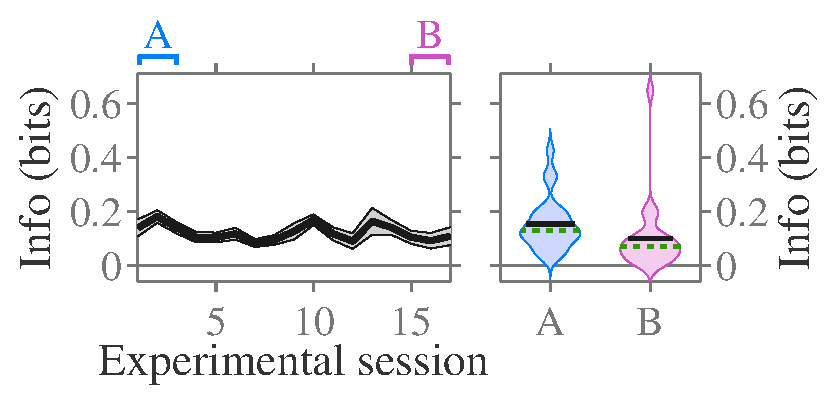
\includegraphics[scale=.45]{%
figs/info2/initial/I_sessionwise_blanco_v1_chmean23_s343-359_oc0_G_1bins_of_527ms_dr_pt_rmvet2_rmvms2_imscn_clhot.eps}}
    \hspace*{\fill}\hspace{.2cm}\hspace*{\fill}
    \subfloat[][\ac{M2} \ac{V1}.\label{fig:info_sess_1x527_v1_jack}]{%
        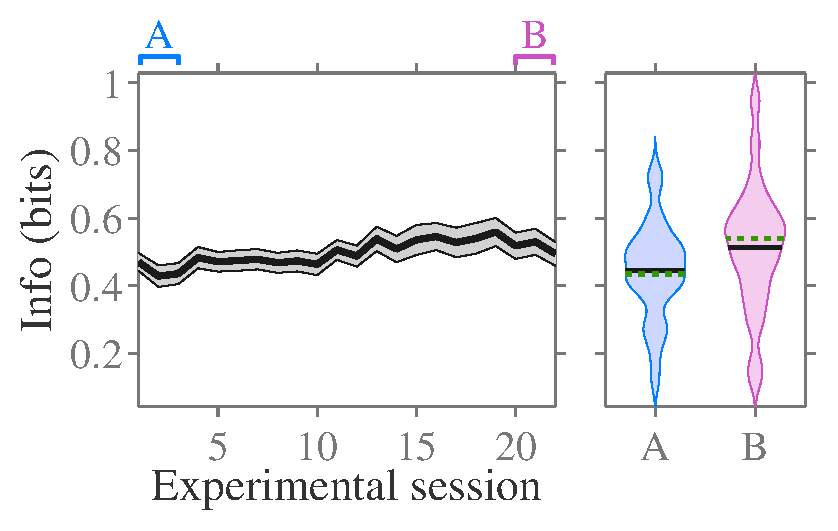
\includegraphics[scale=.45]{%
figs/info2/initial/I_sessionwise_jack_v1_chmean25_s51-72_oc0_G_1bins_of_527ms_dr_pt_rmvet2_rmvms2_imscn_clhot.eps}}
    \hspace*{\fill}
    \\
    \hspace*{\fill}
    \subfloat[][\ac{M1} \ac{V4}.\label{fig:info_sess_1x527_v4_blanco}]{%
        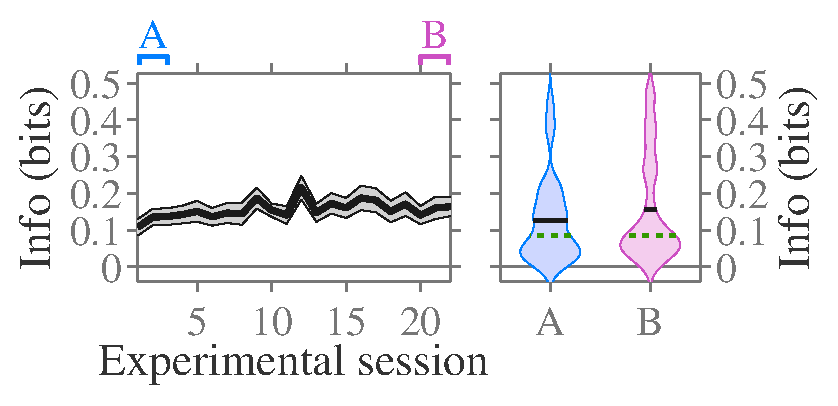
\includegraphics[scale=.45]{%
figs/info2/initial/I_sessionwise_blanco_v4_chmean30_s307,308,311,313,314,317,318,320,321,329-341_oc0_G_1bins_of_527ms_dr_pt_rmvet2_rmvms2_imscn_clhot.eps}}
    \hspace*{\fill}\hspace{.2cm}\hspace*{\fill}
    \subfloat[][\ac{M2} \ac{V4}.\label{fig:info_sess_1x527_v4_jack}]{%
        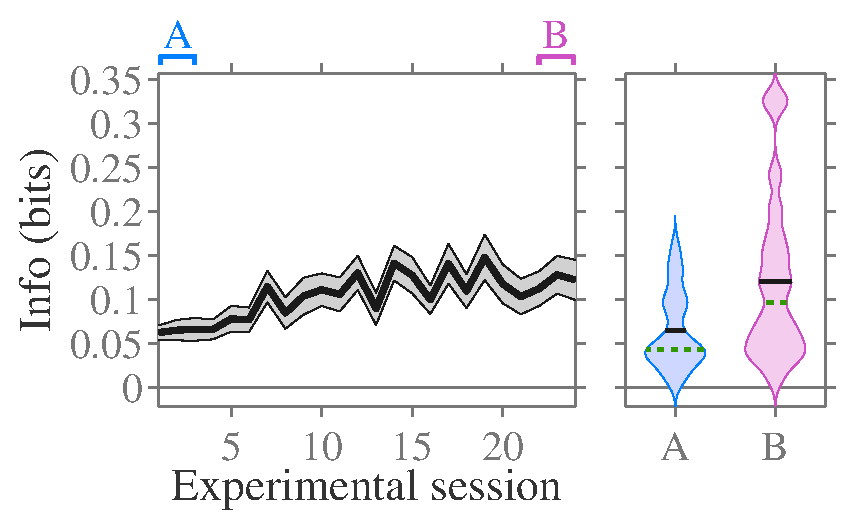
\includegraphics[scale=.45]{%
figs/info2/initial/I_sessionwise_jack_v4_chmean20_s24,25,27-38,40-49_oc0_G_1bins_of_527ms_dr_pt_rmvet2_rmvms2_imscn_clhot.eps}}
    \hspace*{\fill}
    \caption{Information about the test stimulus contained in the firing rate during test presentation and its progression over training sessions.
% The mutual information with the test stimulus is taken for a spike timing based code for a \SI{20}{ms} window of spiking activity, sampled with the start of the window offset ($y$-axis) from \SI{0}{ms} up to \SI{500}{ms} after test stimulus onset.
% The sampling is in intervals of \SI{5}{ms}, so any 4 adjacent squares within each session are highly correlated.
% The recording session number for the data is given along the $x$-axis, and the number of days the animal has been trained for increases from left to right.
% Average mutual information across all the channels is denoted by the pseudo-colour of each of the rectangular patches, centred around the $(x,y)$ co-ordinate to which the measurement relates.
Main panels: information, averaged over channels (\protect\subref{fig:info_sess_1x527_v1_blanco}~\num{23} channels, \protect\subref{fig:info_sess_1x527_v1_jack}~\num{25} channels, \protect\subref{fig:info_sess_1x527_v4_blanco}~\num{30} channels, \protect\subref{fig:info_sess_1x527_v4_jack}~\num{20} channels), with standard error across channels indicated by the shaded region.
Right hand panels: distribution over channels of the information contained in the first three sessions (\zonename{A}) versus last three sessions (\zonename{B}), with mean (solid black line) and median (dashed green line) over channels indicated.
The violin plot shows a Gaussian kernel density, using a bandwidth determined as described in \autoref{sec:info-methods}.
The \ac{PT} bias correction method was used, without further correction to the residual bias.
}
    \label{fig:info_sess_1x527}
\end{figure}


As described in \autoref{sec:pl_dprime_discuss}, the non-significant reduction of information witnessed for \ac{M1} \ac{V1} is most likely explained by the unavoidable reduction of recording signal quality over time.
However, one channel had a large increase in information content against the trend observed for other channels on this electrode array (see \autoref{fig:info_sess_1x527_v1_blanco}, right panel).
This channel is one of a minority whose response profile changes completely between consecutive sessions, and so the sudden large increase in information is most likely due to a small movement in the electrode contact changing which neurons are measured in the data.
We address this discrepancy next.


%------------------------------------
\subsection{Removing inconsistent channels}

We noted that some channels were moving between sessions.
In general, it is just as likely for electrode contacts to move into locations where they are more informative as to move such that they are less informative.
However, to make the results more comparable across sessions, we chose to remove channels whose raster profile (such as those shown in \autoref{sec:pl_rasters}) and overall firing rate in response to the \SI{30}{\percent} sample stimulus changed clearly and suddenly from one session to the next.
We manually selected a small number of channels on this basis, and removed them from the analysis.
For each dataset, the number of channels included afterwards is indicated in \autoref{tab:nchannels_restricted}.


\begin{table}[bthp]
\begin{center}
\begin{tabular}{ccrr}
\toprule
Region  & Animal    & Channels before   & Channels after \\
\midrule
V1      & M1        & 23                & 14 \\
        & M2        & 25                & 20 \\
V4      & M1        & 30                & 25 \\
        & M2        & 20                & 18 \\
\bottomrule
\end{tabular}
\end{center}
\caption{Number of channels before and after restriction on the basis of consistent or smoothly changing firing rates across sessions.}
\label{tab:nchannels_restricted}
\end{table}


\begin{figure}[htbp]%
    \centering
    \hspace*{\fill}
    \subfloat[][\ac{M1} \ac{V1}.\label{fig:info_sess_1x527_restrictchn_v1_blanco}]{%
        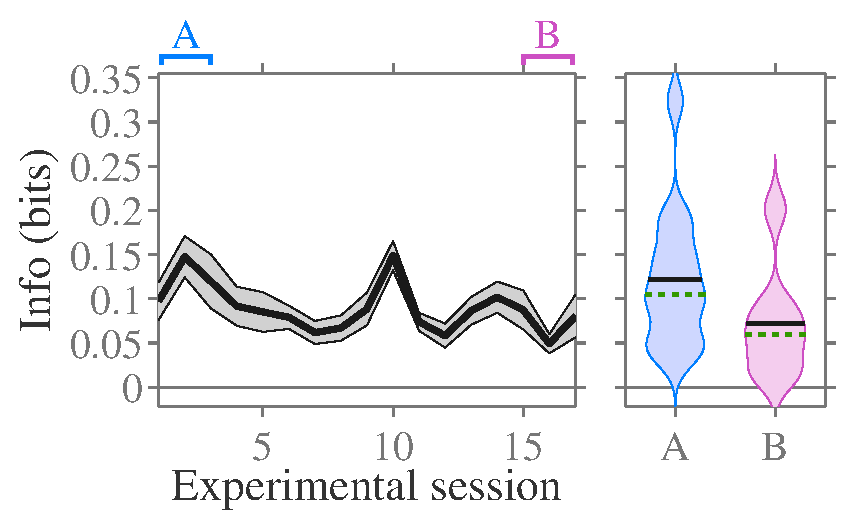
\includegraphics[scale=.45]{%
figs/info2/initial/I_sessionwise_blanco_v1_chmean14_s343-359_oc0_G_1bins_of_527ms_dr_pt_rmvet2_rmvms2_imscn_clhot.eps}}
    \hspace*{\fill}\hspace{.2cm}\hspace*{\fill}
    \subfloat[][\ac{M2} \ac{V1}.\label{fig:info_sess_1x527_restrictchn_v1_jack}]{%
        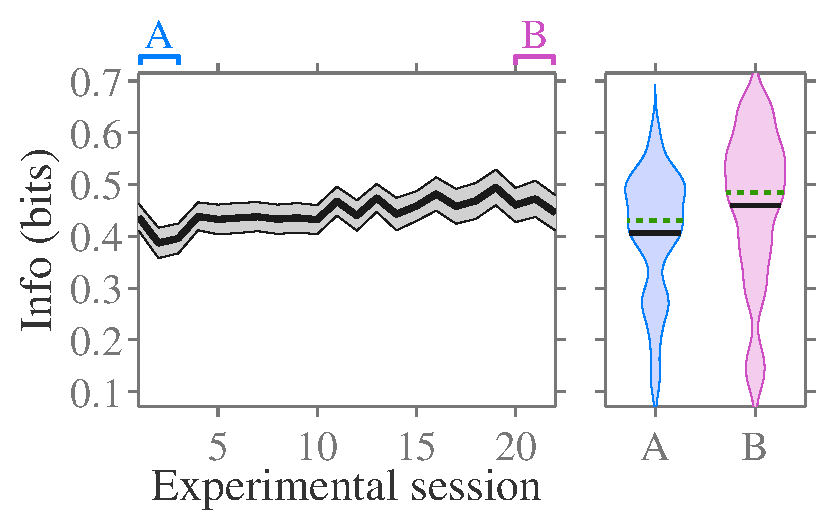
\includegraphics[scale=.45]{%
figs/info2/initial/I_sessionwise_jack_v1_chmean20_s51-72_oc0_G_1bins_of_527ms_dr_pt_rmvet2_rmvms2_imscn_clhot.eps}}
    \hspace*{\fill}
    \\
    \hspace*{\fill}
    \subfloat[][\ac{M1} \ac{V4}.\label{fig:info_sess_1x527_restrictchn_v4_blanco}]{%
        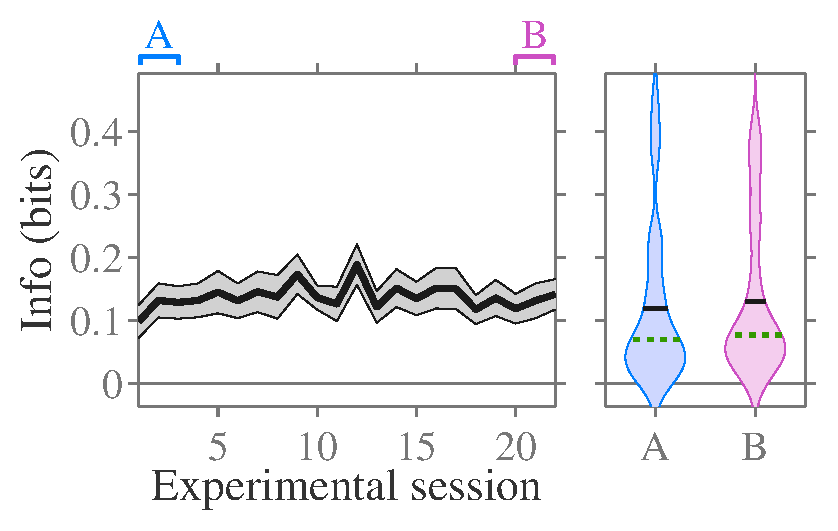
\includegraphics[scale=.45]{%
figs/info2/initial/I_sessionwise_blanco_v4_chmean25_s307,308,311,313,314,317,318,320,321,329-341_oc0_G_1bins_of_527ms_dr_pt_rmvet2_rmvms2_imscn_clhot.eps}}
    \hspace*{\fill}\hspace{.2cm}\hspace*{\fill}
    \subfloat[][\ac{M2} \ac{V4}.\label{fig:info_sess_1x527_restrictchn_v4_jack}]{%
        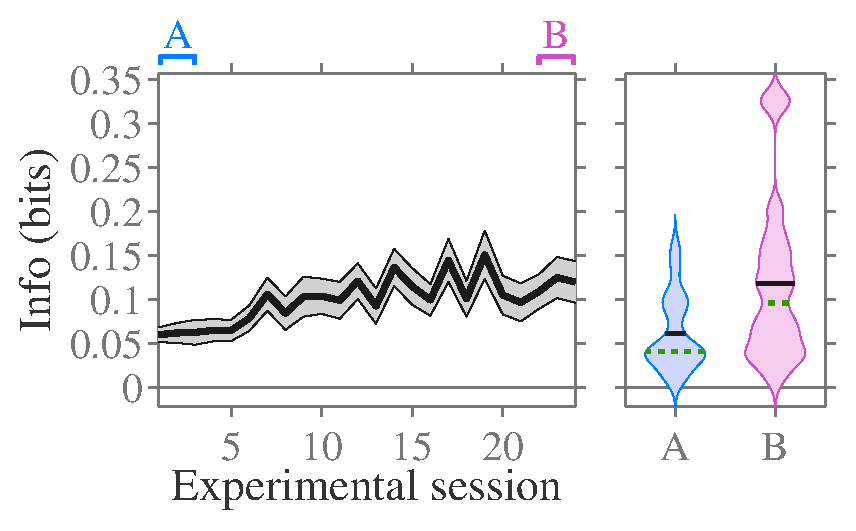
\includegraphics[scale=.45]{%
figs/info2/initial/I_sessionwise_jack_v4_chmean18_s24,25,27-38,40-49_oc0_G_1bins_of_527ms_dr_pt_rmvet2_rmvms2_imscn_clhot.eps}}
    \hspace*{\fill}
    \caption{Information, after removing inconsistent channels, about the test stimulus contained in the firing rate during test presentation and its progression over training sessions.
Main panels: the average over channels (\protect\subref{fig:info_sess_1x527_restrictchn_v1_blanco}~\num{14} channels, \protect\subref{fig:info_sess_1x527_restrictchn_v1_jack}~\num{20} channels, \protect\subref{fig:info_sess_1x527_restrictchn_v4_blanco}~\num{25} channels, \protect\subref{fig:info_sess_1x527_restrictchn_v4_jack}~\num{18} channels) with standard error across channels indicated by the shaded region.
Right hand panels: distribution over channels of the information contained in the first three sessions (\zonename{A}) versus last three sessions (\zonename{B}), with mean (solid black line) and median (dashed green line) over channels indicated.
The \ac{PT} bias correction method was used, without further correction to the residual bias.
}
    \label{fig:info_sess_1x527_restrictchn}
\end{figure}

% blanco v1 1x527.00ms
% dr pt
% same bandwidth bw = 0.018561 used for all cols
% h=1.000000  p=0.014856=1.485642e-02   delta = -0.049242+/-0.017549 = -40.514232%+/-14.587530%
%
% jack v1 1x527.00ms
% dr pt
% same bandwidth bw = 0.033931 used for all cols
% h=1.000000  p=0.000970=9.696090e-04   delta = +0.052784+/-0.013545 = +12.980690%+/-4.272728%
%
% blanco v4 1x527.00ms
% dr pt
% same bandwidth bw = 0.033252 used for all cols
% h=0.000000  p=0.556266=5.562658e-01   delta = +0.010819+/-0.018130 = +9.059702%+/-15.387211%
%
% jack v4 1x527.00ms
% dr pt
% same bandwidth bw = 0.012428 used for all cols
% h=1.000000  p=0.001046=1.046127e-03   delta = +0.056465+/-0.014315 = +91.889667%+/-23.318749%

Besides the channel for \ac{M1} \ac{V1} with an aberrantly large increase in information mentioned above, there is little impact on the results (\autoref{fig:info_sess_1x527_restrictchn}) compared with previously (\autoref{fig:info_sess_1x527}).
For this dataset, \ac{M1} \ac{V1}, the removal of the outlier means the reduction in information over time is now statistically significant (\SI{-0.049\pm0.018}{bits} or \SI{-41\pm15}{\percent}, $p=0.015$).
For the other datasets, there were no notable changes.


%------------------------------------
\subsection{Correcting stimulus class imbalance}
\label{sec:pl_class_imbalance}

As mentioned in \autoref{sec:pl_task}, the stimulus presentation procedure was to include a fixed number of repetitions of each stimulus in a block of trials and present them in a random order.
At the end of each block, additional trials were presented for stimuli which the subject responded to incorrectly.
Since stimuli with a contrast far from the pedestal contrast of \SI{30}{\percent} are much easier for the subject, trials which were repeated at the end of the block were not uniformly distributed across the stimuli.
Overall, this means that harder stimuli close to \SI{30}{\percent} contrast are presented more often than the easier stimuli, as depicted in \autoref{fig:class_balance}.


% blanco v4
% Outer stimuli: A->B 0.497413
% Inner stimuli: A->B 0.094376
% blanco v1
% Outer stimuli: A->B 1.537775
% Inner stimuli: A->B -0.292156
% jack v4
% Session 26 could not be found on disc for jack v4.
% Session 39 could not be found on disc for jack v4.
% Outer stimuli: A->B -2.775447
% Inner stimuli: A->B 5.471745
% jack v1
% Outer stimuli: A->B 2.413654
% Inner stimuli: A->B -2.481668

\begin{figure}[htbp]%
    \centering
    \hspace*{\fill}
    \subfloat[][\ac{M1} \ac{V1}.\label{fig:class_balance_v1_blanco}]{%
        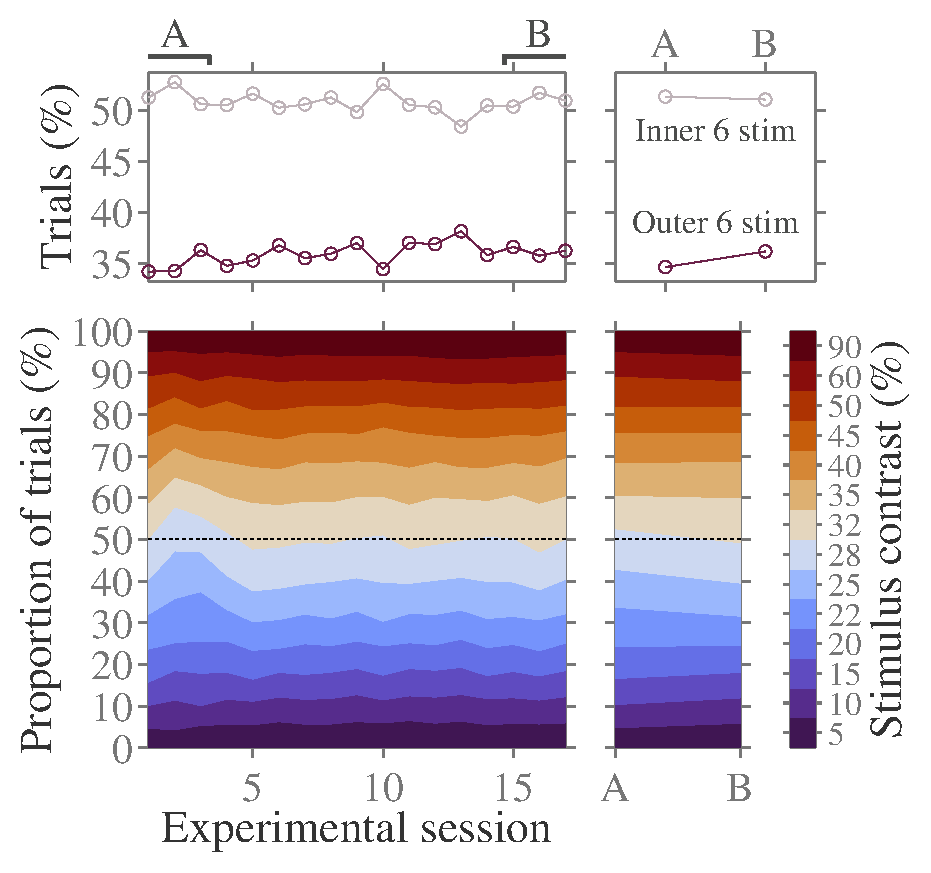
\includegraphics[scale=.45]{%
figs/class_balance/ntrialscond_prop_blanco_v1_oc0_rmvet2_.eps}}
    \hspace*{\fill}\hspace{.2cm}\hspace*{\fill}
    \subfloat[][\ac{M2} \ac{V1}.\label{fig:class_balance_v1_jack}]{%
        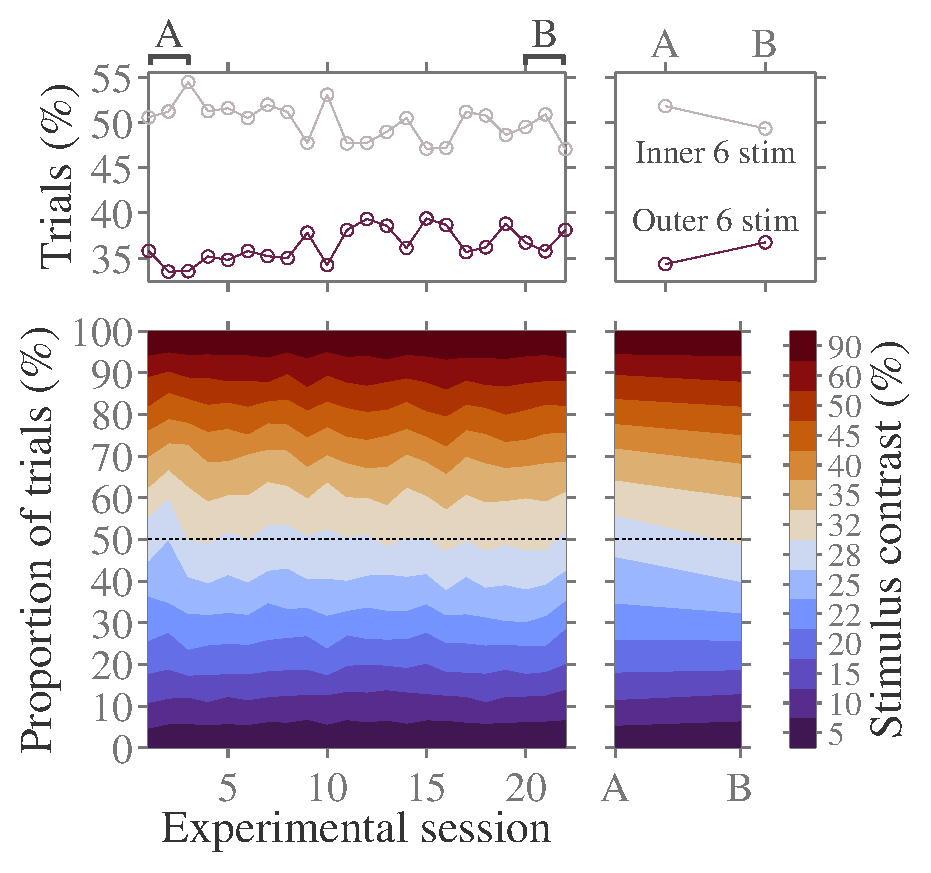
\includegraphics[scale=.45]{%
figs/class_balance/ntrialscond_prop_jack_v1_oc0_rmvet2_.eps}}
    \hspace*{\fill}
    \\
    \hspace*{\fill}
    \subfloat[][\ac{M1} \ac{V4}.\label{fig:class_balance_v4_blanco}]{%
        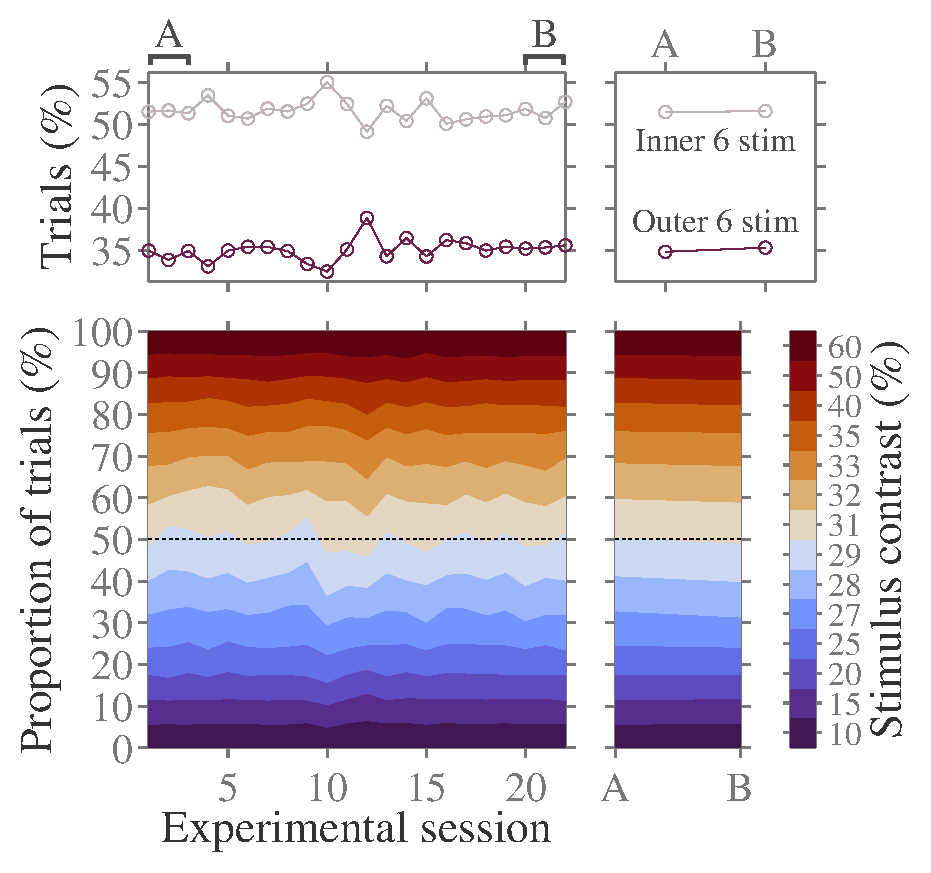
\includegraphics[scale=.45]{%
figs/class_balance/ntrialscond_prop_blanco_v4_oc0_rmvet2_.eps}}
    \hspace*{\fill}\hspace{.2cm}\hspace*{\fill}
    \subfloat[][\ac{M2} \ac{V4}.\label{fig:class_balance_v4_jack}]{%
        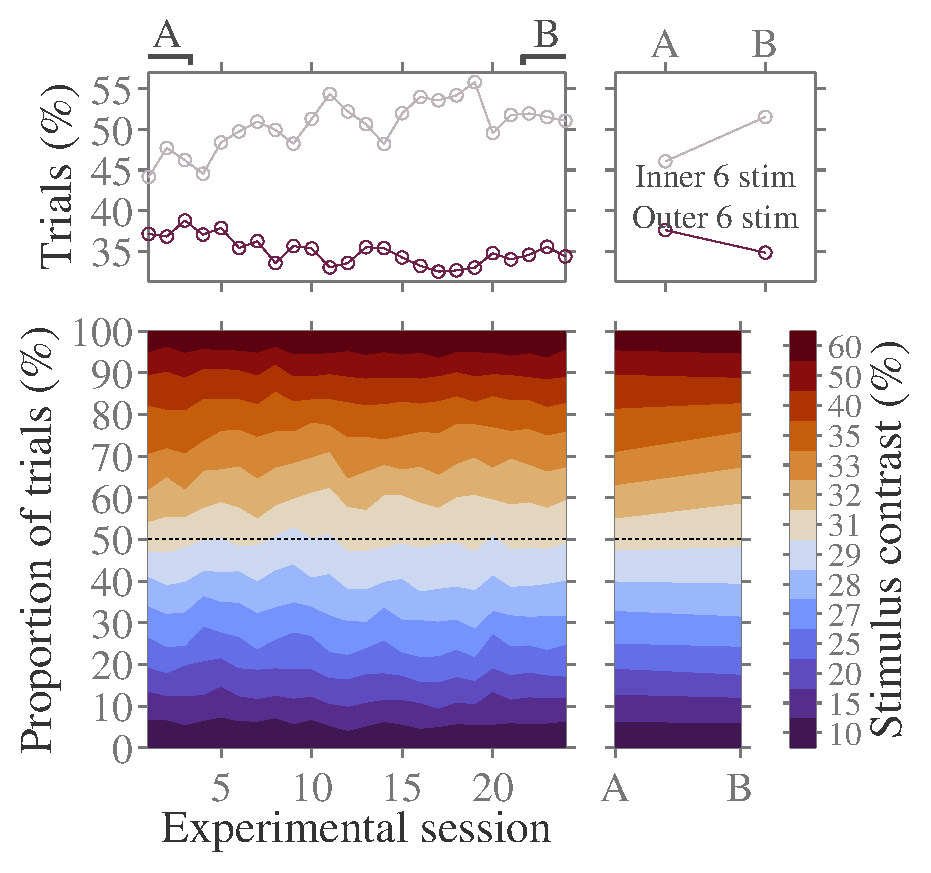
\includegraphics[scale=.45]{%
figs/class_balance/ntrialscond_prop_jack_v4_oc0_rmvet2_.eps}}
    \hspace*{\fill}
    \caption{Proportion of trials in each stimulus class.
Main panels: the proportion (\%) of trials which belong to each stimulus class, with colours indicated to the right, as a function of experimental session.
Above panels: the ``inner \num{6}'' contrasts closest to \SI{30}{\percent} (grey) and ``outer \num{6}'' contrasts furthest from \SI{30}{\percent} (purple).
See \autoref{tab:pl_stim} for the \num{6} contrasts in each group by brain region.
Right hand panels: proportion of trials presented during the first (\zonename{A}) and last (\zonename{B}) three sessions.
}
    \label{fig:class_balance}
\end{figure}


To compute the amount of information about the stimulus contained in the animal's response, we do not need to have a uniform distribution across stimuli.
However, the subject becomes better at the task with training, and the change in relative performance is necessarily not uniform across sessions.
For \ac{M1}, the proportion of trials which belong to each stimulus class was very similar throughout the experiment, as shown in \autoref{fig:class_balance_v1_blanco} and \autoref{fig:class_balance_v4_blanco}.
However for \ac{M2}, this was not the case.
During training with the \ac{V1} stimulation protocol, there was a larger increase in performance for the harder contrast stimuli, which were consequently presented less frequently by the end of training --- the percentage of stimuli with a contrast in one of the hardest 6 categories (closest to \SI{30}{\percent} contrast) fell by \SI{2.5}{\percent} in absolute terms.
This change in stimulus class distribution may seem small, but the size of this change is comparable to the amount of change in information we previously computed.
When training \ac{M2} with the \ac{V4} stimuli, the overall performance was initially lower.
Consequently, the largest increase in performance was that attained for the easier stimuli, and the percentage of trials featuring one of the 6 easiest stimuli (furthest from \SI{30}{\percent} contrast) fell by \SI{5.4}{\percent} in absolute terms.

Changes in the distribution of classes between sessions can impact our analysis in two ways.
Firstly, as described \autoref{eq:info} the amount of information between stimulus, $\SET{S}$, and response, $\SET{R}$, is dependent on the entropy of the stimulus, $\HH(\SET{S})$.
As the distribution of stimulus classes moves closer to uniform, the stimulus entropy increases.
Since our stimulus distribution generally tends to become flatter after training, this may cause an the measured information to become inflated as training progresses.
Secondly, as seen for \ac{M2} \ac{V1}, the proportion of trials which are in the easier categories is higher for later sessions.
These stimuli will have the most distinguishable responses, and their increasing prevalence in the dataset may also produce an artificial increase in information with training.

We corrected the class imbalance on a session-by-session basis by subsampling the trials for more frequent stimulus classes down to the frequency of the least common stimulus class.
The trials included in the subsample were selected at random across the set of trials for each stimulus, without replacement.


\begin{figure}[htbp]%
    \centering
    \hspace*{\fill}
    \subfloat[][\ac{M1} \ac{V1}.\label{fig:info_sess_1x527_balanced_v1_blanco}]{%
        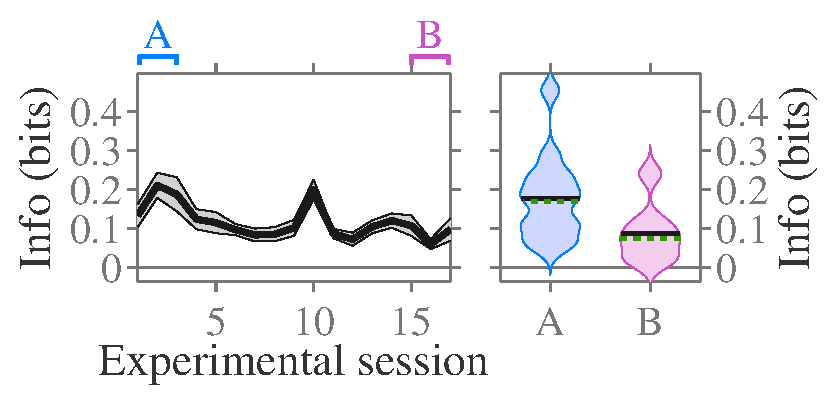
\includegraphics[scale=.45]{%
figs/info2/initial/I_sessionwise_blanco_v1_chmean14_s343-359_oc0_Gbalanced_1bins_of_527ms_dr_pt_rmvet2_rmvms2_imscn_clhot.eps}}
    \hspace*{\fill}\hspace{.2cm}\hspace*{\fill}
    \subfloat[][\ac{M2} \ac{V1}.\label{fig:info_sess_1x527_balanced_v1_jack}]{%
        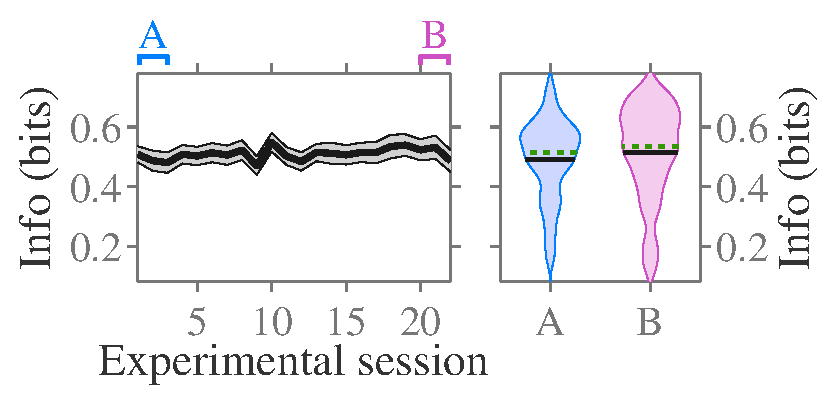
\includegraphics[scale=.45]{%
figs/info2/initial/I_sessionwise_jack_v1_chmean20_s51-72_oc0_Gbalanced_1bins_of_527ms_dr_pt_rmvet2_rmvms2_imscn_clhot.eps}}
    \hspace*{\fill}
    \\
    \hspace*{\fill}
    \subfloat[][\ac{M1} \ac{V4}.\label{fig:info_sess_1x527_balanced_v4_blanco}]{%
        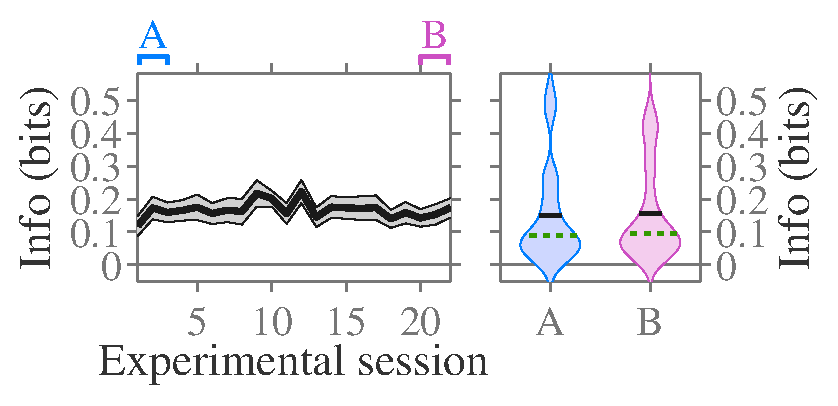
\includegraphics[scale=.45]{%
figs/info2/initial/I_sessionwise_blanco_v4_chmean25_s307,308,311,313,314,317,318,320,321,329-341_oc0_Gbalanced_1bins_of_527ms_dr_pt_rmvet2_rmvms2_imscn_clhot.eps}}
    \hspace*{\fill}\hspace{.2cm}\hspace*{\fill}
    \subfloat[][\ac{M2} \ac{V4}.\label{fig:info_sess_1x527_balanced_v4_jack}]{%
        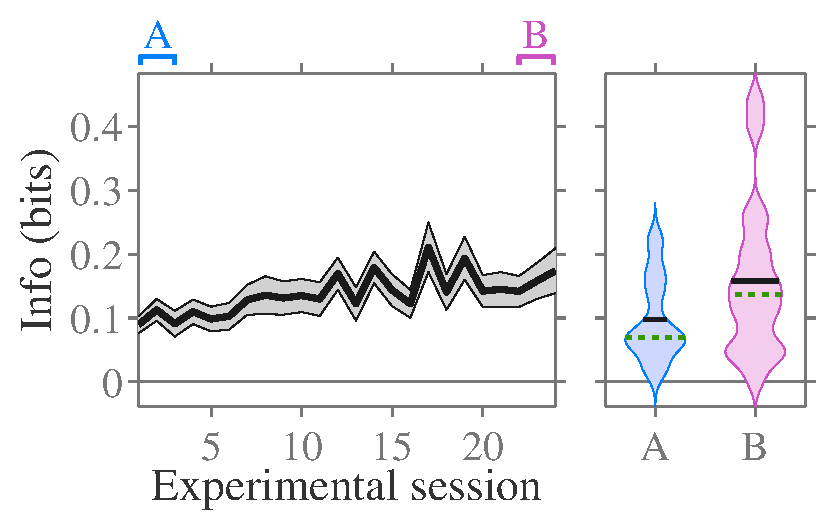
\includegraphics[scale=.45]{%
figs/info2/initial/I_sessionwise_jack_v4_chmean18_s24,25,27-38,40-49_oc0_Gbalanced_1bins_of_527ms_dr_pt_rmvet2_rmvms2_imscn_clhot.eps}}
    \hspace*{\fill}
    \caption{Information, after correcting for the stimulus class balance in each session, about the test stimulus contained in the firing rate during test presentation and its progression over training sessions.
Sub-panels are arranged as per \autoref{fig:info_sess_1x527_restrictchn}, with the same number of channels included.
The \ac{PT} bias correction method was used, without further correction to the residual bias.
}
    \label{fig:info_sess_1x527_balanced}
\end{figure}

% blanco v1 1x527.00ms
% dr pt
% same bandwidth bw = 0.02234 used for all cols
% h=1.000000  p=0.001794=1.794017e-03   delta = -0.089123+/-0.022797 = -50.472174%+/-13.226381%
%
% jack v1 1x527.00ms
% dr pt
% same bandwidth bw = 0.038202 used for all cols
% h=0.000000  p=0.179003=1.790031e-01   delta = +0.022181+/-0.015896 = +4.511570%+/-4.419345%
%
% blanco v4 1x527.00ms
% dr pt
% same bandwidth bw = 0.038581 used for all cols
% h=0.000000  p=0.779391=7.793914e-01   delta = +0.006273+/-0.022144 = +4.185196%+/-15.076193%
%
% jack v4 1x527.00ms
% dr pt
% same bandwidth bw = 0.018676 used for all cols
% h=1.000000  p=0.004131=4.130838e-03   delta = +0.060078+/-0.018145 = +61.470204%+/-18.627960%


Overall, we find the amount of information increases when the class imbalance is corrected for (compare the y-scales of \autoref{fig:info_sess_1x527_balanced} with those of \autoref{fig:info_sess_1x527_restrictchn}).
This is because the stimulus entropy, $\HH(\SET{S})$, has increased when the stimulus distribution became uniform.

As anticipated, correcting for changes in the class balance over time reduces the relative increase in information between the beginning and end of training.
For \ac{V1}, the change in information over training seen in \ac{M1} is reduced more (\SI{-0.089\pm0.023}{bits} or \SI{-50\pm13}{\percent}, $p=0.0018$) and the increase in information for \ac{M2} is no longer statistically significant (\SI{+0.022\pm0.016}{bits} or \SI{+4.5\pm4.4}{\percent}, $p=0.18$).
For \ac{V4}, the outcomes stand unchanged even though the relative change in information is reduced
(\ac{M1}: \SI{+0.006\pm0.022}{bits} or \SI{+4\pm15}{\percent}, $p=0.78$; \ac{M2}: \SI{+0.060\pm0.018}{bits} or \SI{+61\pm19}{\percent}, $p=0.004$).

This post-hoc class rebalancing was applied this throughout the rest of this chapter.
Moreover, the subset of trials which was selected was also maintained, to ensure comparability of results across sections.


%------------------------------------
\subsection{Defending against changes in session duration}

A substantial amount of session-to-session variability in the measurements was observed in our results, depicted in the time-course plots of \autoref{fig:info_sess_1x527}.
A large part of this variability was due to changes in the duration of each session --- some sessions contain \num{5} times as many trials as others.

% blanco v4
% Min # trials for single cond, single session: 17
% Max # trials for single cond, single session: 191
% Min # trials for all cond, single session: 291
% Max # trials for all cond, single session: 1889
% Min # trials for all cond, single rebalanced session: 238
% Max # trials for all cond, single rebalanced session: 1540
% blanco v1
% Min # trials for single cond, single session: 11
% Max # trials for single cond, single session: 147
% Min # trials for all cond, single session: 254
% Max # trials for all cond, single session: 1413
% Min # trials for all cond, single rebalanced session: 154
% Max # trials for all cond, single rebalanced session: 1120
% jack v4
% Min # trials for single cond, single session: 19
% Max # trials for single cond, single session: 125
% Min # trials for all cond, single session: 431
% Max # trials for all cond, single session: 1239
% Min # trials for all cond, single rebalanced session: 266
% Max # trials for all cond, single rebalanced session: 770
% jack v1
% Min # trials for single cond, single session: 18
% Max # trials for single cond, single session: 167
% Min # trials for all cond, single session: 371
% Max # trials for all cond, single session: 1440
% Min # trials for all cond, single rebalanced session: 252
% Max # trials for all cond, single rebalanced session: 1134

% blanco v1, onlycorrect=0 restrict_channels=2
% Min number of codes for single channel: 4
% Max number of codes for single channel: 24
% Min number of trials per code for single channel: 1.200000
% Max number of trials per code for single channel: 17.000000
% jack v1, onlycorrect=0 restrict_channels=2
% Min number of codes for single channel: 5
% Max number of codes for single channel: 30
% Min number of trials per code for single channel: 1.200000
% Max number of trials per code for single channel: 15.400000
% blanco v4, onlycorrect=0 restrict_channels=2
% Min number of codes for single channel: 3
% Max number of codes for single channel: 34
% Min number of trials per code for single channel: 1.285714
% Max number of trials per code for single channel: 26.500000
% jack v4, onlycorrect=0 restrict_channels=2
% Min number of codes for single channel: 5
% Max number of codes for single channel: 24
% Min number of trials per code for single channel: 1.461538
% Max number of trials per code for single channel: 13.888889

% blanco v1, onlycorrect=0 restrict_channels=2 FLAG_MATCH_NT=1
% Min number of codes for single channel: 4
% Max number of codes for single channel: 23
% Min number of trials per code for single channel: 1.100000
% Max number of trials per code for single channel: 13.333333
% jack v1, onlycorrect=0 restrict_channels=2 FLAG_MATCH_NT=1
% Min number of codes for single channel: 5
% Max number of codes for single channel: 30
% Min number of trials per code for single channel: 1.200000
% Max number of trials per code for single channel: 16.200000
% blanco v4, onlycorrect=0 restrict_channels=2 FLAG_MATCH_NT=1
% Min number of codes for single channel: 3
% Max number of codes for single channel: 32
% Min number of trials per code for single channel: 1.214286
% Max number of trials per code for single channel: 18.333333
% jack v4, onlycorrect=0 restrict_channels=2 FLAG_MATCH_NT=1
% Min number of codes for single channel: 5
% Max number of codes for single channel: 22
% Min number of trials per code for single channel: 1.315789
% Max number of trials per code for single channel: 8.833333

Although we were utilising the \ac{PT} bias correction technique, this typically requires \num{4} trials per response for each stimulus condition to be completely effective \citep{Panzeri2007}.
When analysing the amount of information contained in the overall firing rate, the cardinality of the set of spike counts per channel --- the number of possible numbers of spikes during the test stimulus presentation --- ranges from \num{3} to \num{50}.
The number of trials in one session for an individual stimulus varies from \num{11} to \num{191}, with the total number of trials per session ranging from \num{254} to \num{1889}.
Consequently, the number of trials per response to a single stimulus varies from \num{1.2} to \num{26.5}.
After correcting for the stimulus class imbalance, the number of trials we are considering from each session falls, ranging from \num{154} to \num{1540}, exasperating the problem.
With this, the number of trials per response ranges from \num{1.1} to \num{18.3}.
Not only is there a \num{20} fold difference in the number of trials per response, but some sessions have stimuli with only a quarter of the number of repetitions we should be using for the bias correction to be effective \citep{Panzeri2007}.

This shortage of trials per stimulus condition results means the \ac{PT} bias correction method underestimates the bias for the shorter sessions, leading to an overestimate in the reported information.
This is illustrated in \autoref{fig:I_vs_invN}, where we compare with the estimated information with the reciprocal number of trials, $\nicefrac{1}{N}$, and find a linear correlation.
This is in keeping with the literature, since $\I_{\text{measured}}$ is known to be proportional to $\nicefrac{1}{N}$ if no bias correction is performed \citep{Treves1995}.


\begin{figure}[htbp]
    \centering
    \hspace*{\fill}
    \subfloat[][\ac{M1} \ac{V1}.\label{fig:I_vs_invN_v1_blanco}]{%
        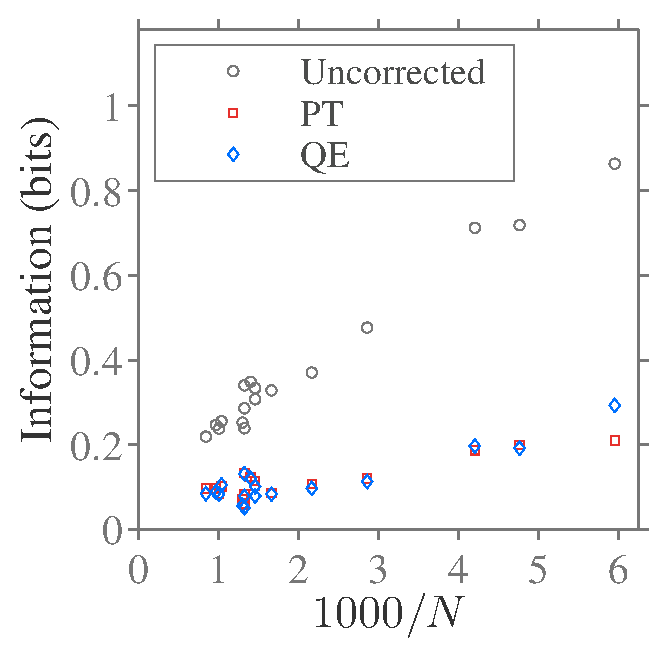
\includegraphics[scale=.45]{%
figs/info2/bias/ntrials_I_vs_invN_combindivpap_leg_blanco_v1_14chn_Gbalanced_1bins_of_527ms.eps}}
    \hspace*{\fill}\hspace{.2cm}\hspace*{\fill}
    \subfloat[][\ac{M2} \ac{V1}.\label{fig:I_vs_invN_v1_jack}]{%
        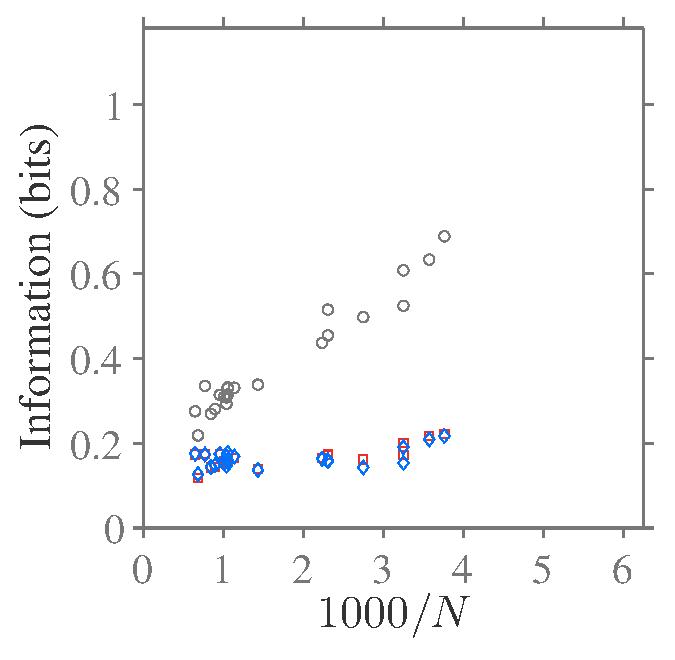
\includegraphics[scale=.45]{%
figs/info2/bias/ntrials_I_vs_invN_combindivpap_blanco_v4_25chn_Gbalanced_1bins_of_527ms.eps}}
    \hspace*{\fill}
    \\
    \hspace*{\fill}
    \subfloat[][\ac{M1} \ac{V4}.\label{fig:I_vs_invN_v4_blanco}]{%
        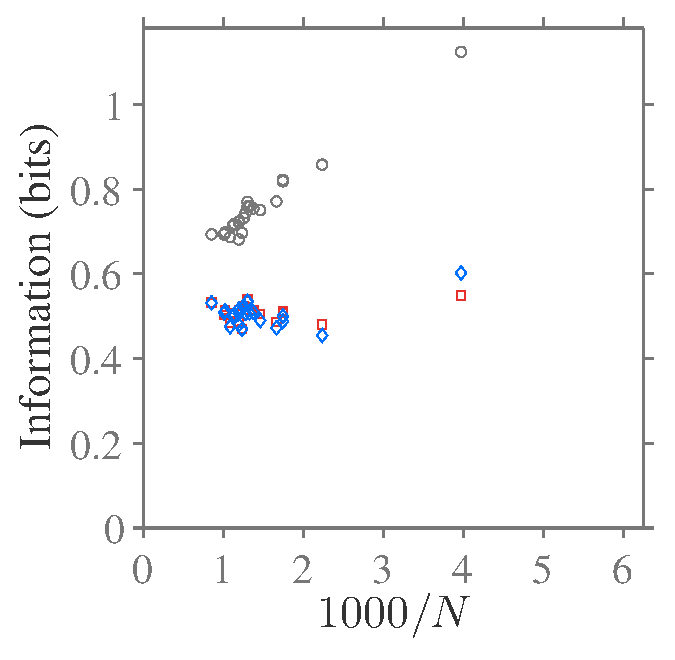
\includegraphics[scale=.45]{%
figs/info2/bias/ntrials_I_vs_invN_combindivpap_jack_v1_20chn_Gbalanced_1bins_of_527ms.eps}}
    \hspace*{\fill}\hspace{.2cm}\hspace*{\fill}
    \subfloat[][\ac{M2} \ac{V4}.\label{fig:I_vs_invN_v4_jack}]{%
        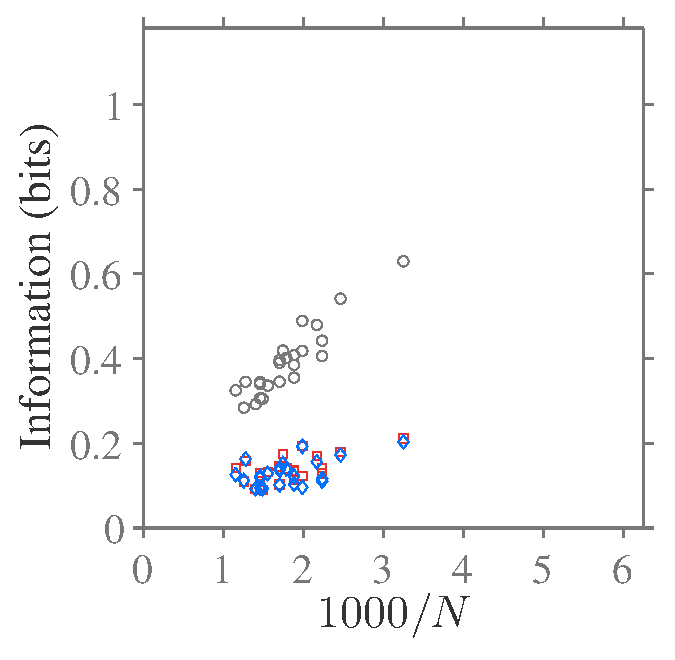
\includegraphics[scale=.45]{%
figs/info2/bias/ntrials_I_vs_invN_combindivpap_jack_v4_18chn_Gbalanced_1bins_of_527ms.eps}}
    \hspace*{\fill}
    \caption{Distribution of measured information as a function of $\nicefrac{1}{N}$, where $N$ is the number of trials in the session.
Results are shown both without correcting for the finite measurement bias (grey circles), using \ac{PT} bias correction (red squares), and using \ac{QE} bias correction (blue diamonds).
Information was computed after using subsampling to address the stimulus class imbalance (see \autoref{sec:pl_class_imbalance}), and this is reflected in the value of $N$.
}
    \label{fig:IvN}
    \label{fig:I_vs_invN}
\end{figure}


There are several potential ways we can correct for the change in bias incurred by the changes in number of trials.
\begin{itemize}
\item Subsample all sessions down to the same number of trials (rarefy).
\item Use bootstrapping, randomising the mapping between stimulus and response, to estimate the residual bias and subtract this from the reported information.
\item Group together stimuli above and below \SI{30}{\percent} contrast so we only have two stimulus classes, each with approximately \num{7} times more trials than before.
\item Group together trials across consecutive sessions so we have the same number of trials in each information computation step.
\end{itemize}

The first method is clearly undesirable, since we would be throwing away most of our data and knowingly operating in the regime where the bias correction method breaks down for all sessions instead of only a few.
In such a scenario, the bias on the estimated information would be larger than the actual information and our comparison across sessions would have little validity.
Instead, we focus on the three other --- more practical --- methods, whose outcomes are described below.


%------------------------------------
\subsection{Bootstrap correction}
\label{sec:pl_bootstrapping}

Shuffling the responses across stimuli destroys the information contained in the response about the stimulus.
By performing such shuffling and computing the amount of information between the randomly paired labels, we can estimate the bias \citep{Optican1991}.
Using this in conjunction with a bias correction technique such as \ac{PT} both when performing the original and bootstrapped information calculation allows us to estimate the residual bias after on the corrected value.
As described in \autoref{sec:info-bias} and by \citet{Panzeri1996}, this will typically lead to an overestimate of the bias.
However, since our residual bias will be significantly reduced beforehand due to the \ac{PT} technique, the overestimation is on a much smaller residual bias and impacts the results less.

\begin{figure}[htbp]
    \centering
    \hspace*{\fill}
    \subfloat[][\ac{M1} \ac{V1}.\label{fig:I_vs_invN_btsp_v1_blanco}]{%
        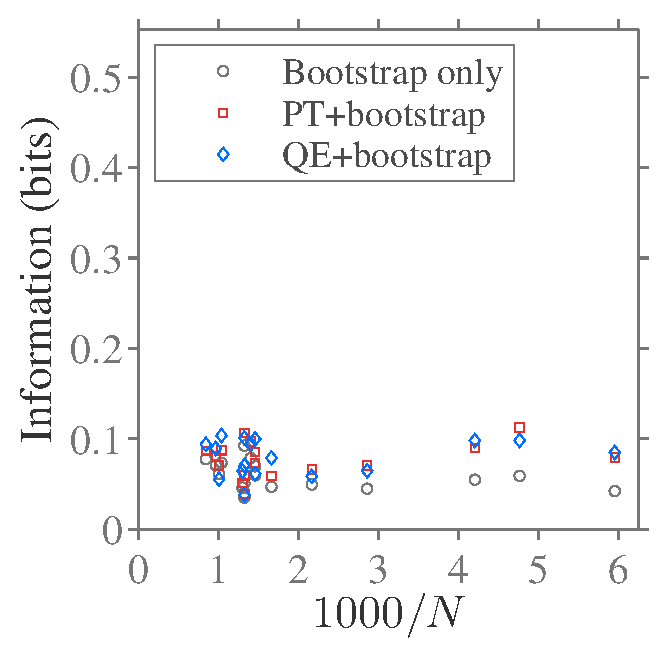
\includegraphics[scale=.45]{%
figs/info2/bias/ntrials_I_vs_invN_combindivpap_leg_blanco_v1_14chn_Gbalanced_1bins_of_527ms_btsp20.eps}}
    \hspace*{\fill}\hspace{.2cm}\hspace*{\fill}
    \subfloat[][\ac{M2} \ac{V1}.\label{fig:I_vs_invN_btsp_v1_jack}]{%
        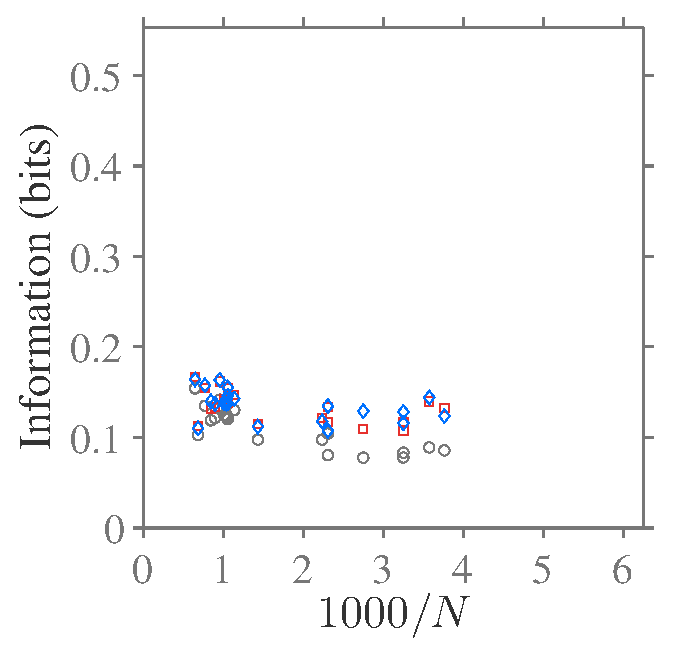
\includegraphics[scale=.45]{%
figs/info2/bias/ntrials_I_vs_invN_combindivpap_blanco_v4_25chn_Gbalanced_1bins_of_527ms_btsp20.eps}}
    \hspace*{\fill}
    \\
    \hspace*{\fill}
    \subfloat[][\ac{M1} \ac{V4}.\label{fig:I_vs_invN_btsp_v4_blanco}]{%
        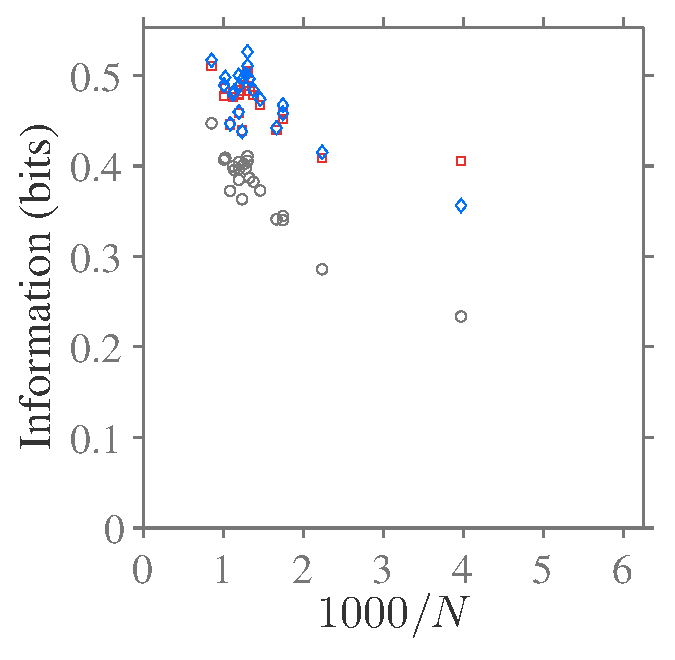
\includegraphics[scale=.45]{%
figs/info2/bias/ntrials_I_vs_invN_combindivpap_jack_v1_20chn_Gbalanced_1bins_of_527ms_btsp20.eps}}
    \hspace*{\fill}\hspace{.2cm}\hspace*{\fill}
    \subfloat[][\ac{M2} \ac{V4}.\label{fig:I_vs_invN_btsp_v4_jack}]{%
        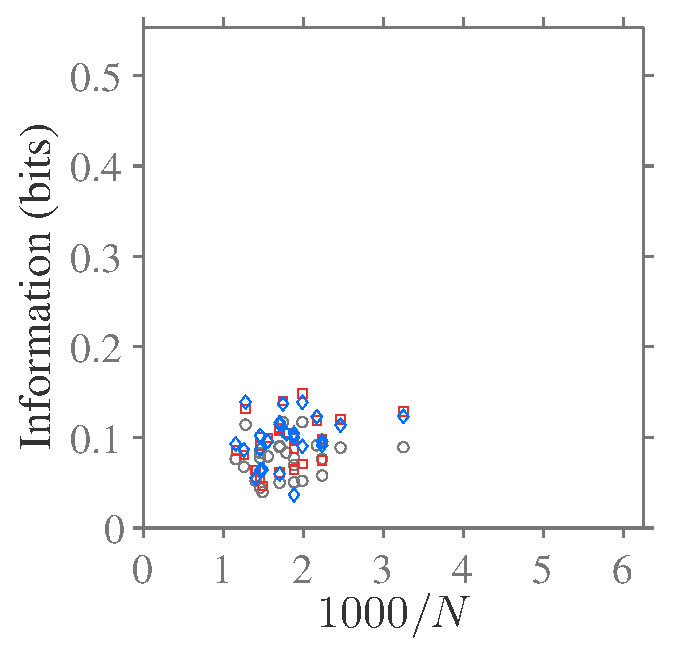
\includegraphics[scale=.45]{%
figs/info2/bias/ntrials_I_vs_invN_combindivpap_jack_v4_18chn_Gbalanced_1bins_of_527ms_btsp20.eps}}
    \hspace*{\fill}
    \caption{
    Distribution of measured information, with bootstrap bias correction, as a function of $\nicefrac{1}{N}$, where $N$ is the number of trials in the session.
Results are shown with bias correction either achieved solely from subtracting the information contained in response-shuffled copies of the data (bootstraps; grey circles), or by combining this with a more principled bias correction technique (\ac{PT}, red squares; \ac{QE}, blue diamonds).
}
    \label{fig:I_vs_invN_btsp}
\end{figure}

We find that using bootstrapping for the bias correction does indeed overestimate the bias, resulting in a negative correlation between information and $\nicefrac{1}{N}$.
This effect is particularly dominant for the \ac{M1} \ac{V4} dataset (see \autoref{fig:I_vs_invN_btsp_v4_blanco}).

%------------------------------------
\subsection{Grouping stimuli together}
\label{sec:pl_bias_grouping}

During the experiment, the subject is tasked with determining whether the stimulus contrast is higher or lower than the \SI{30}{\percent} sample stimulus presented at the start of each trial.
As a consequence of this, the subject does not need to learn exactly what stimulus is on screen, only whether the stimulus is in the half above or below \SI{30}{\percent} contrast.
For instance, since the target output is the same for \SI{31}{\percent} and \SI{32}{\percent} contrast stimuli, there is no need for the subject to discriminate between them, but there is motivation for the subject to learn to discriminate between these and the \SI{29}{\percent} contrast stimulus.

We refer to the subset of information which assists in decoding whether the stimulus was higher or lower than the \SI{30}{\percent} threshold as the task-pertinent information, and discuss this in \autoref{sec:task-info}.
For now, we will only consider the impact on the residual information bias when we restrict ourselves to measuring only the task-pertinent information.
In this calculation, we determine how much information the firing rate provides is with about which group the stimulus is in (higher or lower) instead of the information about precisely which of the \num{14} stimuli was on screen.
Grouping the stimuli together in this way should reduce the residual bias, since there are only two class labels, and \num{7} times as many trials per class.


\begin{figure}[htbp]
    \centering
    \hspace*{\fill}
    \subfloat[][\ac{M1} \ac{V1}.\label{fig:I_vs_invN_target-group_v1_blanco}]{%
        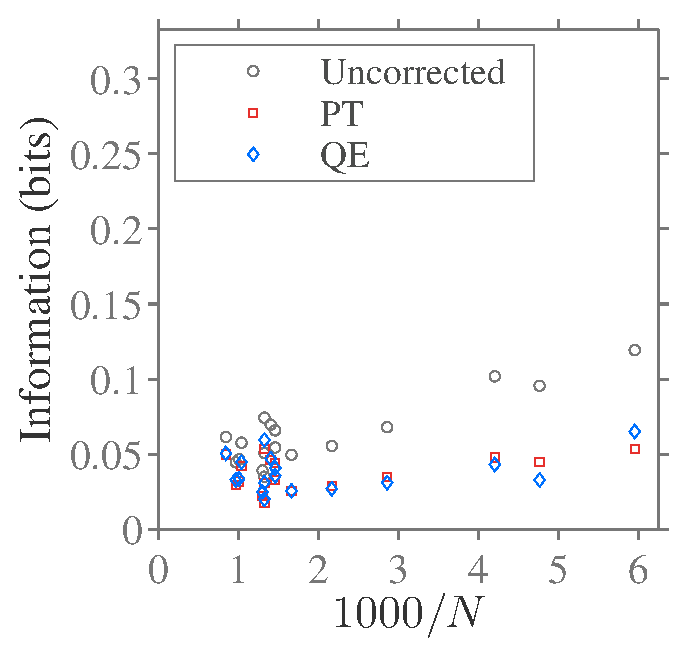
\includegraphics[scale=.45]{%
figs/info2/bias/ntrials_I_vs_invN_combindivpap_leg_blanco_v1_14chn_Gclass-group-balanced_1bins_of_527ms.eps}}
    \hspace*{\fill}\hspace{.2cm}\hspace*{\fill}
    \subfloat[][\ac{M2} \ac{V1}.\label{fig:I_vs_invN_target-group_v1_jack}]{%
        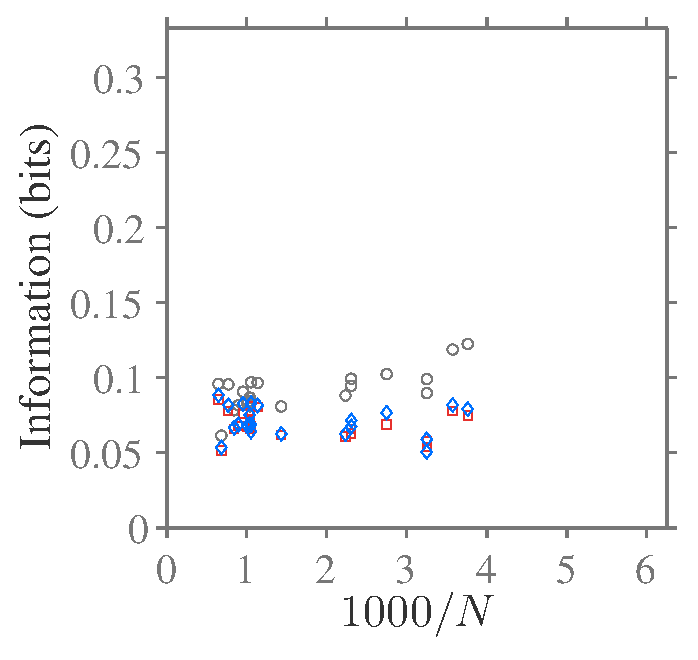
\includegraphics[scale=.45]{%
figs/info2/bias/ntrials_I_vs_invN_combindivpap_blanco_v4_25chn_Gclass-group-balanced_1bins_of_527ms.eps}}
    \hspace*{\fill}
    \\
    \hspace*{\fill}
    \subfloat[][\ac{M1} \ac{V4}.\label{fig:I_vs_invN_target-group_v4_blanco}]{%
        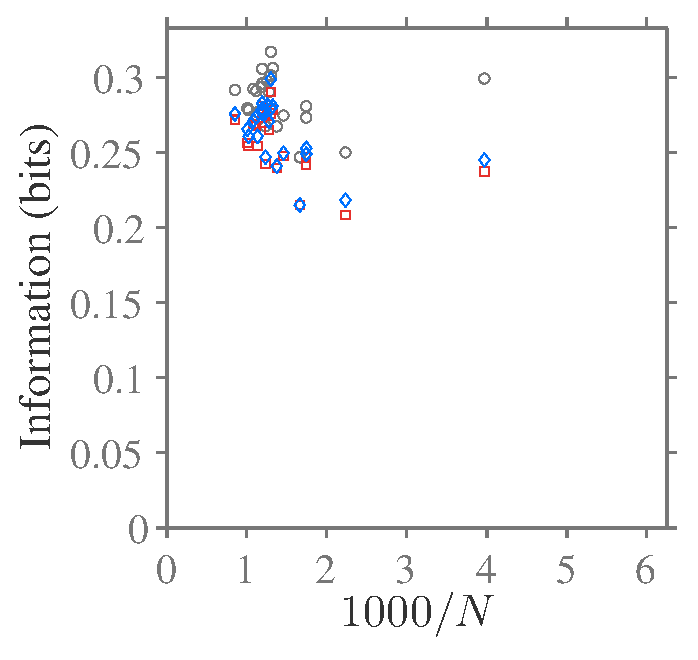
\includegraphics[scale=.45]{%
figs/info2/bias/ntrials_I_vs_invN_combindivpap_jack_v1_20chn_Gclass-group-balanced_1bins_of_527ms.eps}}
    \hspace*{\fill}\hspace{.2cm}\hspace*{\fill}
    \subfloat[][\ac{M2} \ac{V4}.\label{fig:I_vs_invN_target-group_v4_jack}]{%
        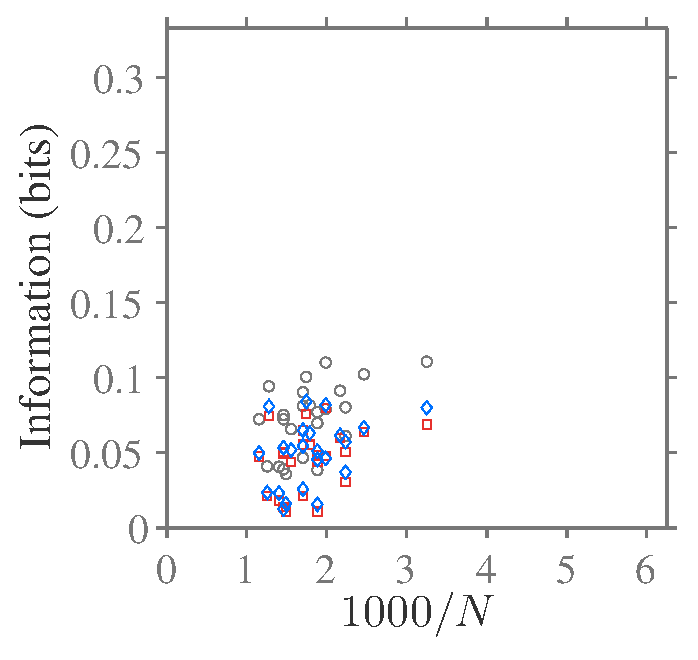
\includegraphics[scale=.45]{%
figs/info2/bias/ntrials_I_vs_invN_combindivpap_jack_v4_18chn_Gclass-group-balanced_1bins_of_527ms.eps}}
    \hspace*{\fill}
    \caption{Distribution of task-pertinent information measured as a function of $\nicefrac{1}{N}$, where $N$ is the number of trials in the session.
Results are shown both without correcting for the finite measurement bias (grey circles), using \ac{PT} bias correction (red squares), and using \ac{QE} bias correction (blue diamonds).
}
    \label{fig:I_vs_invN_target-group}
\end{figure}


As anticipated, using only two stimulus classes to increase the number of trials per stimulus class greatly reduces the residual bias after \ac{PT} bias correction.
This is witnessed in the reduced correlation between estimated information and $\nicefrac{1}{N}$ seen in \autoref{fig:I_vs_invN_target-group}.

%------------------------------------
\subsection{Trial-wise analysis}

We now consider what happens if we group together trials from multiple sessions into a single block and analyse them together.
Doing so allows us overcome the difference in bias between sessions, since the same number of trials would be used in each block and this can be set large enough to ensure we are in the correct domain for bias correction perform adequately.
There are typically no more than \num{25} different firing rates for any single channel, so we grouped together \num{100} trials of each stimulus condition.

Using this methodology, we focus on the subject's performance as a function of the number of trials which they have completed since the beginning of the experiment, irrespective of how many training sessions these trials are spread across.
Therefore, such a technique makes sense if we consider learning to occur during sessions and not to occur between them.
However, such a view is in contrast with the hypothesis that one of the important functions of sleep is to facilitate consolidation of memories and learning from during the day.
Should this be an important contributor towards perceptual learning, one would expect the breaks between sessions not to be irrelevant but to instead enable an increase in performance even without exposure to the training stimuli.


\begin{figure}[htbp]%
    \centering
    \hspace*{\fill}
    \subfloat[][\ac{M1} \ac{V1}.\label{fig:info_trial_1x527_balanced_v1_blanco}]{%
        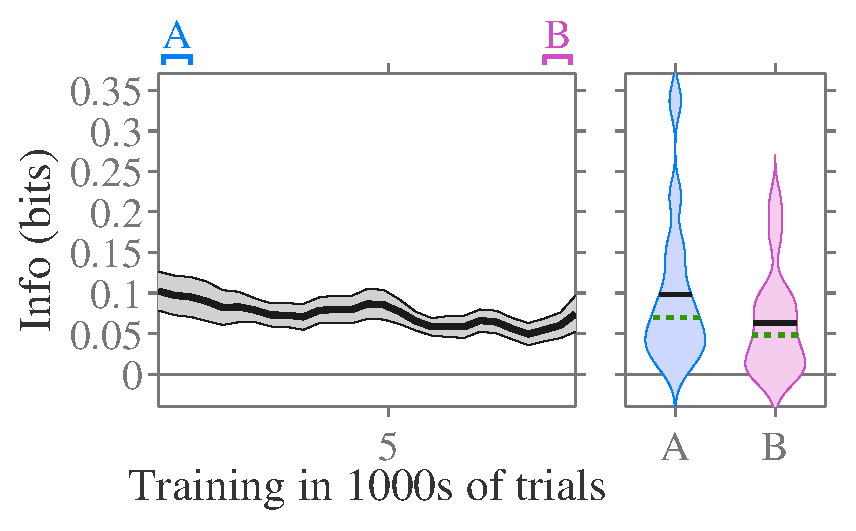
\includegraphics[scale=.45]{%
figs/info2/bias/I_trialwise_blanco_v1_chmean14_s343-354,355.1,355.2,356-359_tp4_1bins_of_527ms_dr_pt_oc0_Gbalanced_test_tc5-5-20,22-3-28,32,35-5-50,60,90_nt1400_ts350_rmvet2_rmvms2_imscn_clhot.eps}}
    \hspace*{\fill}\hspace{.2cm}\hspace*{\fill}
    \subfloat[][\ac{M2} \ac{V1}.\label{fig:info_trial_1x527_balanced_v1_jack}]{%
        \includegraphics[scale=.45]{%
figs/info2/bias/I_trialwise_jack_v1_chmean20_s51-72_tp4_1bins_of_527ms_dr_pt_oc0_Gbalanced_test_tc5-5-20,22-3-28,32,35-5-50,60,90_nt1400_ts350_rmvet2_rmvms2_imscn_clhot.eps}}
    \hspace*{\fill}
    \\
    \hspace*{\fill}
    \subfloat[][\ac{M1} \ac{V4}.\label{fig:info_trial_1x527_balanced_v4_blanco}]{%
        \includegraphics[scale=.45]{%
figs/info2/bias/I_trialwise_blanco_v4_chmean25_s307,308,311,313,314,317,318,320,321,329-341_tp4_1bins_of_527ms_dr_pt_oc0_Gbalanced_test_tc10-5-25,27-29,31-33,35,40-10-60_nt1400_ts350_rmvet2_rmvms2_imscn_clhot.eps}}
    \hspace*{\fill}\hspace{.2cm}\hspace*{\fill}
    \subfloat[][\ac{M2} \ac{V4}.\label{fig:info_trial_1x527_balanced_v4_jack}]{%
        \includegraphics[scale=.45]{%
figs/info2/bias/I_trialwise_jack_v4_chmean18_s24,25,27-38,40-49_tp4_1bins_of_527ms_dr_pt_oc0_Gbalanced_test_tc10-5-25,27-29,31-33,35,40-10-60_nt1400_ts350_rmvet2_rmvms2_imscn_clhot.eps}}
    \hspace*{\fill}
    \caption{Information about the test stimulus contained in the firing rate during test presentation and its progression over training sessions, estimated across blocks of \num{100} consecutive trials of each stimulus class taken by merging consecutive sessions together to accumulate sufficiently many trials.
Main panels: the average over channels (\protect\subref{fig:info_trial_1x527_balanced_v1_blanco}~\num{14} channels, \protect\subref{fig:info_trial_1x527_balanced_v1_jack}~\num{20} channels, \protect\subref{fig:info_trial_1x527_balanced_v4_blanco}~\num{25} channels, \protect\subref{fig:info_trial_1x527_balanced_v4_jack}~\num{18} channels) with standard error across channels indicated by the shaded region.
Right hand panels: distribution over channels of the information contained in the first three blocks of \num{1400} trials (\zonename{A}) versus last three blocks (\zonename{B}), with mean (solid black line) and median (dashed green line) over channels indicated.
The violin plot shows a Gaussian kernel density, using a bandwidth determined as described in \autoref{sec:info-methods}.
The \ac{PT} bias correction method was used, without further correction to the residual bias.
The stimulus class imbalance was address on a session-by-session basis by subsampling as described previously (\autoref{sec:pl_class_imbalance}) before merging sessions together.
}
    \label{fig:info_trial_1x527_balanced}
\end{figure}


Since we performed the spike extraction such that the spontaneous firing rate is held constant across sessions for each channel, the firing rate during stimulus presentation is comparable between sessions.
This means it is plausible that, when decoding the information, the extracted firing rate corresponding to the stimuli could be similar across consecutive sessions.

We find that grouping trials together in this way smooths out the problems with inter-session changes in residual bias on the information estimate.
But because of both changes in neural connectivity and small movement in the electrode contacts between sessions, the neural code is not guaranteed to be the same between sessions.
Indeed, we observed a peak in the estimated information corresponding to longer sessions where the trial sample size is smaller than or a similar size to the number of trials grouped together in each block (not shown\footnote{This phenomena occurred when the analysis was repeated with a smaller number of trials grouped together, and is not present in \autoref{fig:info_trial_1x527_balanced} due to the smoothing effect of using such large blocks of \num{1400} trials.}).
For this reason, it is prudent not to proceed with such a methodology.


%------------------------------------------------------------------------------
\section{Task-pertinent and nonpertinent information}
\label{sec:task-info}

So far, we have been computing the amount of information in the neural response (the firing rate over the stimulus presentation period) about the identity of the presented stimulus.
Computing the mutual information between these two tells us how much information we gain about which stimulus was presented when we are told how many spikes were detected on a given electrode contact.
However, the object the subject is tasked with --- to identify whether the presented stimulus has a contrast higher or lower than the pedestal contrast --- is somewhat different.
To achieve this goal, it is not necessary to distinguish exactly which stimulus was presented.

We can separate the information given by the neural response into two parts: task-pertinent and task-nonpertinent information.
The task-pertinent information helps one tell whether the stimulus was in the half above or below the pedestal contrast of \SI{30}{\percent}.
However we also gain information about exactly which stimuli within the upper and lower half of the set of contrasts is more likely to have been presented.
Although this information helps one distinguish which stimulus was presented (and hence presumably helps the subject perceive the stimuli more accurately), it is not pertinent to the subject's task.

For instance, any information which helps one discriminate between whether a \SI{29}{\percent} or \SI{31}{\percent} contrast stimulus was more likely to have been presented is pertinent to the task.
Whereas if we gain information about the stimulus which updates the probability of it having a \SI{28}{\percent} versus a \SI{29}{\percent} contrast without changing the probability that it was one of \SI{28}{\percent} or \SI{29}{\percent} contrast, this is not pertinent to the task.

Although it is only a binary response (a choice of one of two saccade targets), it is still possible for the behavioural response to encode both task-pertinent and task-nonpertinent information.
For instance, let us assume that the subject performs the task at a rate higher than chance.
Then, a behavioural response of ``\textit{test contrast is lower}'' tells us a contrast in the lower half was more likely to have been presented, providing task-pertinent information.
Additionally, since contrasts further from the \SI{30}{\percent} threshold are easier for the subject, we can empirically observe that a response of ``\textit{test contrast is lower}'' is more likely to be elicited if the contrast was further below the threshold than if it was close to the threshold.\footnote{This trivially follows using Bayes' rule.}
This difference in relative likelihood supplies us with additional, task-nonpertinent, information about which stimulus was presented.


\subsection{Methods for decomposing task-pertinent information}
\label{sec:task-info-methods}

First, we computed the total information contained in the neural response as before, using the total spikes recorded by a single channel over \SI{527}{\milli\second} of stimulus presentation as the response on each trial.
The finite sampling bias on the estimated information was corrected for using the \ac{PT} method, and further residual bias removed using bootstrapping (see \autoref{sec:pl_bootstrapping}).
Stimulus class imbalance was corrected for using subsampling, as described in \autoref{sec:pl_class_imbalance}.

The amount of task-pertinent information contained in the response was estimated by shuffling the stimulus labels against the responses, whilst preserving which side of \SI{30}{\percent} contrast the stimulus label was on.
This destroys any information about the stimulus beyond that pertinent to the task --- choosing whether the stimulus was above or below \SI{30}{\percent} contrast --- but maintains the number of class labels and samples per class.
Consequently, the bias on the information will be similar to that when computing the total information, and the results will be more directly comparable.\footnote{However, the bias will not be the same for the two information values because after shuffling the range of possible values for the response will have increased. Consequently, it is still necessary to do individual bias correction with \ac{PT} and bootstrapping on each of the information computations.}
We repeated this with \num{20} permutations, each with their own set of \num{20} bootstraps, and took the average over them.
The amount of task-nonpertinent information was estimated by subtracting the task-pertinent information (found with shuffling) from the total information (found without shuffling).

To compute the proportion of information in the response which was pertinent to the task, we divided the estimated task-pertinent information by the total information (after correcting for the bias on each estimate).
To prevent channels whose responses contain negligible information about the stimulus contaminating the results with anomalously large (or small) outliers after the division, we excluded any channels whose total information was less than \num{1.5} times the standard deviation across the bootstrapped information values.
This threshold was determined empirically; \num{3} standard deviations unnecessarily removed too many channels, whereas \num{1} standard deviation retained channels with too little information whose task-pertinence proportion was unstable (at or beyond $0$ and $1$), which increased the overall variance.
Approximately half the channels were removed with this step (\ac{M1} \ac{V1}: $14\to4$, \ac{M2} \ac{V1}: $20\to20$, \ac{M1} \ac{V4}: $25\to13$, \ac{M2} \ac{V4}: $18\to7$).
Additionally, the proportional information reported for each channel was capped at $0$ and $1$ before taking the average over channels.
Although it is impossible for the proportion of information which is task-pertinent to fall outside the range $[0, 1]$, our measurements of the information are fuzzy.
In particular, this can arise from subtracting the average over bootstraps, since the bootstraps are stochastic samples and we subtract different bootstraps from the total and task-pertinent information.
With the \num{1.5} standard deviation threshold, we observed that only a single channel fell outside this cap.

To quantify the change over time, we again compared the information averaged over the first three sessions (\zonename{A}) with the information over the last three sessions (\zonename{B}).
For the relative information, only channels which had a significant amount of total information (exceeding \num{1.5} times the standard deviation over bootstraps) for both the average over \zonename{A} and also over\zonename{B} were included.
This step was included to ensure \zonename{A} and \zonename{B} were directly comparable; a paired $t$-test was used to compare the information at \zonename{A} with \zonename{B}.

Similarly, we considered the amount of information about the stimulus contained in the behavioural response of the animal, which was a saccade to one of two targets, indicating whether the subject believed the contrast to be higher or lower than \SI{30}{\percent} (two forced-choice).
The same procedure was used to decomposed the the total information in this response into task-pertinent and nonpertinent components, and find the proportion of the information which was task-pertinent.


\subsection{Results for \acs{V1} information pertinence}

We separated the total information about the stimulus contained in the neural response into task-pertinent and task-nonpertinent components as described in \autoref{sec:task-info-methods}.
For \ac{M1}, there was a non-significant decrease in the total information, task-pertinent information, and the task-nonpertinent information between \zonename{A} and \zonename{B} (paired Student's $t$-test; $p=0.20$, $p=0.38$, and $p=0.13$ respectively), as shown in \autoref{fig:info_taskpertinent_v1_ch_blanco}.
Correspondingly, there was no significant change in the fraction of the total information which was task-pertinent either ($p=0.60$; see \autoref{fig:info_taskpertinent_rel_v1_ch_blanco}).

For \ac{M2}, there was a small, non-significant, decrease in the task-nonpertinent information between \zonename{A} and \zonename{B} (\SI{-0.010\pm0.007}{bits}, $p=0.16$), but there was a significant increase in the task-pertinent information (\SI{+0.060\pm0.011}{bits}, $p = 2 \times 10^-5$; see \autoref{fig:info_taskpertinent_v1_ch_jack}).
Together, these give a combined increase in the total information of \SI{+0.050\pm0.015}{bits} ($p=0.004$).
Since the task-nonpertinent information was stable while the task-pertinent information increased with training, the proportion of encoded information which was task-pertinent increased by \SI{+7.0\pm1.3}{\percent} ($p = 4 \times 10^-5$), as shown in \autoref{fig:info_taskpertinent_rel_v1_ch_jack}.

% blanco v1 1x527.00ms
% dr pt
% For Total Info (bits)
% n=14  h=0.000000  p=0.205484=2.054842e-01   delta = -0.026854+/-0.020149 = -29.290339%+/-22.139211%
% For Task-pertinent Info (bits)
% n=14  h=0.000000  p=0.375025=3.750246e-01   delta = -0.010713+/-0.011662 = -25.593377%+/-27.886183%
% For Task-nonpertinent Info (bits)
% n=14  h=0.000000  p=0.133354=1.333535e-01   delta = -0.016142+/-0.010081 = -32.396084%+/-20.293906%
% selected bw  :  bandwidth=0.011217
%
% For Task-pertinent Info (%)
% n=4  h=0.000000  p=0.596176=5.961759e-01   delta = +4.414025+/-7.470531 = +10.618742%+/-533.852117%
% For Task-nonpertinent Info (%)
% n=4  h=0.000000  p=0.596176=5.961759e-01   delta = -4.414025+/-7.470531 = -7.554155%+/-533.702687%
% selected bw  :  bandwidth=2.813857
%
%
% jack v1 1x527.00ms
% dr pt
% For Total Info (bits)
% n=20  h=1.000000  p=0.003762=3.761940e-03   delta = +0.049989+/-0.015146 = +11.458962%+/-4.411886%
% For Task-pertinent Info (bits)
% n=20  h=1.000000  p=0.000020=2.022440e-05   delta = +0.060332+/-0.010732 = +28.392210%+/-5.205318%
% For Task-nonpertinent Info (bits)
% n=20  h=0.000000  p=0.162219=1.622189e-01   delta = -0.010343+/-0.007113 = -4.622742%+/-3.554708%
% selected bw  :  bandwidth=0.015976
%
% For Task-pertinent Info (%)
% n=20  h=1.000000  p=0.000036=3.596357e-05   delta = +7.049025+/-1.315612 = +14.317851%+/-97.552405%
% For Task-nonpertinent Info (%)
% n=20  h=1.000000  p=0.000036=3.596357e-05   delta = -7.049025+/-1.315612 = -13.884894%+/-97.550225%
% selected bw  :  bandwidth=1.236527

\begin{figure}[htbp]%
    \centering
    \hspace*{\fill}
    \subfloat[][\ac{M1} \ac{V1} Information.\label{fig:info_taskpertinent_v1_ch_blanco}]{%
        \includegraphics[scale=.45]{%
figs/info2/task-pertinent/I_sessionwise_blanco_v1_chmean14_s343-359_oc0_Gclass-shuffled-balanced_1bins_of_527ms_dr_pt_btsp20_rmvet2_rmvms2_info_leg.eps}}
    \hspace*{\fill}\hspace{.2cm}\hspace*{\fill}
    \subfloat[][\ac{M2} \ac{V1} Information.\label{fig:info_taskpertinent_v1_ch_jack}]{%
        \includegraphics[scale=.45]{%
figs/info2/task-pertinent/I_sessionwise_jack_v1_chmean20_s51-72_oc0_Gclass-shuffled-balanced_1bins_of_527ms_dr_pt_btsp20_rmvet2_rmvms2_info.eps}}
    \hspace*{\fill}
    \\
    \hspace*{\fill}
    \subfloat[][\ac{M1} \ac{V1} Relative information.\label{fig:info_taskpertinent_rel_v1_ch_blanco}]{%
        \includegraphics[scale=.45]{%
figs/info2/task-pertinent/I_sessionwise_blanco_v1_chmean14_s343-359_oc0_Gclass-shuffled-balanced_1bins_of_527ms_dr_pt_btsp20_rmvet2_rmvms2_relative-info.eps}}
    \hspace*{\fill}\hspace{.2cm}\hspace*{\fill}
    \subfloat[][\ac{M2} \ac{V1} Relative information.\label{fig:info_taskpertinent_rel_v1_ch_jack}]{%
        \includegraphics[scale=.45]{%
figs/info2/task-pertinent/I_sessionwise_jack_v1_chmean20_s51-72_oc0_Gclass-shuffled-balanced_1bins_of_527ms_dr_pt_btsp20_rmvet2_rmvms2_relative-info.eps}}
    \hspace*{\fill}
    \caption{Breakdown of task-pertinent and nonpertinent information contained in \ac{V1} recording channels.
In \protect\subref{fig:info_taskpertinent_v1_ch_blanco} and \protect\subref{fig:info_taskpertinent_v1_ch_jack}, the total information about the stimulus (grey), task-pertinent information (green), and task-nonpertinent (red) contained in each of \num{14} and \num{20} channels respectively.
In \protect\subref{fig:info_taskpertinent_rel_v1_ch_blanco} and \protect\subref{fig:info_taskpertinent_rel_v1_ch_jack}, the relative information about the stimulus which is task-pertinent (green) and task-nonpertinent (red) contained in channels with a significant amount of total information (\num{4} and \num{20} respectively).
Main panels: across training sessions, the average information over channels, with standard error across channels indicated by the shaded region.
Right hand panels: distribution over channels of the information (or relative information) in the first three sessions (\zonename{A}) versus last three sessions (\zonename{B}), with mean (solid black line) and median (dashed green line) over channels indicated.
The violin plot shows a Gaussian kernel density, using a bandwidth determined as described in \autoref{sec:info-methods}.
The \ac{PT} bias correction method was used, with the residual bias further reduced using bootstrapping (see \autoref{sec:pl_bootstrapping}).
The stimulus class imbalance was corrected using subsampling, as described in \autoref{sec:pl_class_imbalance}.
    \label{fig:info_taskpertinent_v1_ch}
}
\end{figure}


Over the same period of training, we examined the decomposition of the information contained in the behavioural response of the experimental subject.
Similar trends were found for \ac{M1} and \ac{M2}, as shown in \autoref{fig:info_taskpertinent_v1_behav}.
There was a vast increase in the amount of task-pertinent information between \zonename{A} and \zonename{B} of \SI{+0.32}{bits} and \SI{+0.34}{bits} respectively, which more than tripled the amount of task-pertinent information given in the subject's response between the beginning and end of the experiment.
The task-nonpertinent information in the response increased by a modest \SI{+0.06}{bits} and \SI{+0.03}{bits} respectively, which is a relative increase of \SI{71}{\percent} and \SI{32}{\percent} from \zonename{A} to \zonename{B}.
Collectively, this meant the proportion of information which was task-pertinent increased from near \SI{60}{\percent} to near \SI{80}{\percent} for both subjects, as shown in \autoref{fig:info_taskpertinent_rel_v1_behav_blanco} and \subref{fig:info_taskpertinent_rel_v1_behav_jack}.

% Behavioural info for blanco v1
% For Total Info (bits)
% n=1  h=NaN  p=NaN=NaN   delta = +0.381066+/-0.000000 = +172.797622%+/-0.000000%
% For Task-pertinent Info (bits)
% n=1  h=NaN  p=NaN=NaN   delta = +0.323136+/-0.000000 = +230.776949%+/-0.000000%
% For Task-nonpertinent Info (bits)
% n=1  h=NaN  p=NaN=NaN   delta = +0.057930+/-0.000000 = +71.956869%+/-0.000000%
% For Task-pertinent Info (%)
% n=1  h=NaN  p=NaN=NaN   delta = +13.494701+/-0.000000 = +21.253604%+/-0.000000%
% For Task-nonpertinent Info (%)
% n=1  h=NaN  p=NaN=NaN   delta = -13.494701+/-0.000000 = -36.965408%+/-0.000000%
%
% Behavioural info for jack v1
% For Total Info (bits)
% n=1  h=NaN  p=NaN=NaN   delta = +0.366698+/-0.000000 = +139.268115%+/-0.000000%
% For Task-pertinent Info (bits)
% n=1  h=NaN  p=NaN=NaN   delta = +0.335353+/-0.000000 = +201.184738%+/-0.000000%
% For Task-nonpertinent Info (bits)
% n=1  h=NaN  p=NaN=NaN   delta = +0.031345+/-0.000000 = +32.443197%+/-0.000000%
% For Task-pertinent Info (%)
% n=1  h=NaN  p=NaN=NaN   delta = +16.382229+/-0.000000 = +25.877507%+/-0.000000%
% For Task-nonpertinent Info (%)
% n=1  h=NaN  p=NaN=NaN   delta = -16.382229+/-0.000000 = -44.646533%+/-0.000000%

\begin{figure}[htbp]%
    \centering
    \hspace*{\fill}
    \subfloat[][\ac{M1} \ac{V1} Information.\label{fig:info_taskpertinent_v1_behav_blanco}]{%
        \includegraphics[scale=.45]{%
figs/info2/task-pertinent/I_behav_blanco_v1_s343-359_Gclass-shuffled-balanced_dr_pt_btsp20_rmvet2_info.eps}}
    \hspace*{\fill}\hspace{.2cm}\hspace*{\fill}
    \subfloat[][\ac{M2} \ac{V1} Information.\label{fig:info_taskpertinent_v1_behav_jack}]{%
        \includegraphics[scale=.45]{%
figs/info2/task-pertinent/I_behav_jack_v1_s51-72_Gclass-shuffled-balanced_dr_pt_btsp20_rmvet2_info.eps}}
    \hspace*{\fill}
    \\
    \hspace*{\fill}
    \subfloat[][\ac{M1} \ac{V1} Relative information.\label{fig:info_taskpertinent_rel_v1_behav_blanco}]{%
        \includegraphics[scale=.45]{%
figs/info2/task-pertinent/I_behav_blanco_v1_s343-359_Gclass-shuffled-balanced_dr_pt_btsp20_rmvet2_relative-info.eps}}
    \hspace*{\fill}\hspace{.2cm}\hspace*{\fill}
    \subfloat[][\ac{M2} \ac{V1} Relative information.\label{fig:info_taskpertinent_rel_v1_behav_jack}]{%
        \includegraphics[scale=.45]{%
figs/info2/task-pertinent/I_behav_jack_v1_s51-72_Gclass-shuffled-balanced_dr_pt_btsp20_rmvet2_relative-info.eps}}
    \hspace*{\fill}
    \caption{Breakdown of task-pertinent and nonpertinent information contained in behavioural responses during \ac{V1} recording.
In \protect\subref{fig:info_taskpertinent_v1_behav_blanco} and \protect\subref{fig:info_taskpertinent_v1_behav_jack}, the total information about the stimulus (grey), task-pertinent information (green), and task-nonpertinent (red) contained the behavioural response on each trial.
In \protect\subref{fig:info_taskpertinent_rel_v1_behav_blanco} and \protect\subref{fig:info_taskpertinent_rel_v1_behav_jack}, the relative information about the stimulus which is task-pertinent (green) and task-nonpertinent (red).
The \ac{PT} bias correction method was used, with the residual bias further reduced using bootstrapping (see \autoref{sec:pl_bootstrapping}).
The stimulus class imbalance was corrected using subsampling, as described in \autoref{sec:pl_class_imbalance}.
    \label{fig:info_taskpertinent_v1_behav}
}
\end{figure}


\subsection{Results for \acs{V4} information pertinence}

For \ac{M1}, we found no significant change in the total, task-pertinent, or task-nonpertinent information about the stimulus encoded in \ac{V4} channels ($p=0.48$, $p=0.19$, and $p=0.94$ respectively; see \autoref{fig:info_taskpertinent_v4_ch_blanco}).
There was a small, but non-significant, increase of \SI{+0.014\pm0.010}{bits} in the average task-pertinent information between \zonename{A} and \zonename{B}.
Correspondingly, there was no significant change in the fraction of information which was task-pertinent either ($p=0.61$; see \autoref{fig:info_taskpertinent_rel_v4_ch_blanco}).

On the other hand, for \ac{M2} there was a significant ($p=0.0005$) increase in task-pertinent information from \zonename{A} to \zonename{B}, increasing by \SI{+0.054\pm0.013}{bits}, which is approximately \num{5} times its initial value.
Meanwhile, the amount of task-nonpertinent information did not notably change (\SI{+0.008\pm0.008}{bits}, $p=0.32$).
Together, these effects accumulatively produced an significant increase in total information of \SI{+0.062\pm0.018}{bits} ($p=0.003$).
As a consequence of this, the proportion of information which is task-pertinent increased from under \SI{20}{\percent} to around \SI{50}{\percent}, with a swing from \zonename{A} to \zonename{B} of \SI{+33\pm3}{\percent} ($p=5 \times 10^-5$).

Most information is initially not pertinent to the task, which may relate to most channels initially being inhibited by sample stimulus, as described in \autoref{sec:pl_dprime_v4} (\autoref{fig:dprime_v4_jack}).
The largest increase in task-pertinent information occurs on the 5th experimental session.
This corresponds to a session where several channels changed from stimulus-inhibited (negative $d'$) to stimulus-excited (positive $d'$).

% blanco v4 1x527.00ms
% dr pt
% For Total Info (bits)
% n=25  h=0.000000  p=0.480089=4.800887e-01   delta = +0.014921+/-0.020800 = +12.563164%+/-17.729269%
% For Task-pertinent Info (bits)
% n=25  h=0.000000  p=0.192543=1.925430e-01   delta = +0.014002+/-0.010443 = +26.745305%+/-19.984138%
% For Task-nonpertinent Info (bits)
% n=25  h=0.000000  p=0.941701=9.417010e-01   delta = +0.000919+/-0.012434 = +1.383585%+/-18.794865%
% selected bw  :  bandwidth=0.016494
%
% For Task-pertinent Info (%)
% n=13  h=0.000000  p=0.613049=6.130492e-01   delta = -2.717323+/-5.233468 = -5.561730%+/-601.681813%
% For Task-nonpertinent Info (%)
% n=13  h=0.000000  p=0.613049=6.130492e-01   delta = +2.717323+/-5.233468 = +5.313240%+/-601.673483%
% selected bw  :  bandwidth=3.203598
%
% jack v4 1x527.00ms
% dr pt
% For Total Info (bits)
% n=18  h=1.000000  p=0.002821=2.821313e-03   delta = +0.062224+/-0.017844 = +108.817777%+/-31.227202%
% For Task-pertinent Info (bits)
% n=18  h=1.000000  p=0.000527=5.272562e-04   delta = +0.054160+/-0.012710 = +505.870407%+/-118.716410%
% For Task-nonpertinent Info (bits)
% n=18  h=0.000000  p=0.321069=3.210688e-01   delta = +0.008065+/-0.007890 = +17.352317%+/-17.000845%
% selected bw  :  bandwidth=0.004437
%
% For Task-pertinent Info (%)
% n=7  h=1.000000  p=0.000051=5.059743e-05   delta = +33.408297+/-3.262665 = +136.706215%+/-360.592804%
% For Task-nonpertinent Info (%)
% n=7  h=1.000000  p=0.000051=5.059743e-05   delta = -33.408297+/-3.262665 = -44.213106%+/-360.371435%
% selected bw  :  bandwidth=2.699929

\begin{figure}[htbp]%
    \centering
    \hspace*{\fill}
    \subfloat[][\ac{M1} \ac{V4} Information.\label{fig:info_taskpertinent_v4_ch_blanco}]{%
        \includegraphics[scale=.45]{%
figs/info2/task-pertinent/I_sessionwise_blanco_v4_chmean25_s307,308,311,313,314,317,318,320,321,329-341_oc0_Gclass-shuffled-balanced_1bins_of_527ms_dr_pt_btsp20_rmvet2_rmvms2_info_leg.eps}}
    \hspace*{\fill}\hspace{.2cm}\hspace*{\fill}
    \subfloat[][\ac{M2} \ac{V4} Information.\label{fig:info_taskpertinent_v4_ch_jack}]{%
        \includegraphics[scale=.45]{%
figs/info2/task-pertinent/I_sessionwise_jack_v4_chmean18_s24,25,27-38,40-49_oc0_Gclass-shuffled-balanced_1bins_of_527ms_dr_pt_btsp20_rmvet2_rmvms2_info.eps}}
    \hspace*{\fill}
    \\
    \hspace*{\fill}
    \subfloat[][\ac{M1} \ac{V4} Relative information.\label{fig:info_taskpertinent_rel_v4_ch_blanco}]{%
        \includegraphics[scale=.45]{%
figs/info2/task-pertinent/I_sessionwise_blanco_v4_chmean25_s307,308,311,313,314,317,318,320,321,329-341_oc0_Gclass-shuffled-balanced_1bins_of_527ms_dr_pt_btsp20_rmvet2_rmvms2_relative-info_leg.eps}}
    \hspace*{\fill}\hspace{.2cm}\hspace*{\fill}
    \subfloat[][\ac{M2} \ac{V4} Relative information.\label{fig:info_taskpertinent_rel_v4_ch_jack}]{%
        \includegraphics[scale=.45]{%
figs/info2/task-pertinent/I_sessionwise_jack_v4_chmean18_s24,25,27-38,40-49_oc0_Gclass-shuffled-balanced_1bins_of_527ms_dr_pt_btsp20_rmvet2_rmvms2_relative-info.eps}}
    \hspace*{\fill}
    \caption{Breakdown of task-pertinent and nonpertinent information contained in \ac{V4} recording channels.
In \protect\subref{fig:info_taskpertinent_v4_ch_blanco} and \protect\subref{fig:info_taskpertinent_v4_ch_jack}, the total information about the stimulus (grey), task-pertinent information (green), and task-nonpertinent (red) contained in each of \num{25} and \num{18} channels respectively.
In \protect\subref{fig:info_taskpertinent_rel_v4_ch_blanco} and \protect\subref{fig:info_taskpertinent_rel_v4_ch_jack}, the relative information about the stimulus which is task-pertinent (green) and task-nonpertinent (red) contained in channels with a significant amount of total information (\num{13} and \num{7} respectively).
Main panels: across training sessions, the average information over channels, with standard error across channels indicated by the shaded region.
Right hand panels: distribution over channels of the information (or relative information) in the first three sessions (\zonename{A}) versus last three sessions (\zonename{B}), with mean (solid black line) and median (dashed green line) over channels indicated.
The violin plot shows a Gaussian kernel density, using a bandwidth determined as described in \autoref{sec:info-methods}.
The \ac{PT} bias correction method was used, with the residual bias further reduced using bootstrapping (see \autoref{sec:pl_bootstrapping}).
The stimulus class imbalance was corrected using subsampling, as described in \autoref{sec:pl_class_imbalance}.
    \label{fig:info_taskpertinent_v4_ch}
}
\end{figure}


The behavioural information for \ac{V4} training sessions shows a similar trend to the behavioural information during \ac{V1} training sessions.
Namely, there is a larger increase in task-pertinent information and a smaller increase in task-nonpertinent information.

For \ac{M1}, the subject began training with a decent initial performance, and correspondingly a decent amount of task-pertinent information is given by the behavioural response, as shown in \autoref{fig:info_taskpertinent_v4_behav_blanco}.
Indeed, for \ac{M1} around \SI{75}{\percent} of the information contained in the behavioural response is task-pertinent at the beginning of training, and this percentage does not notably change throughout training (see \autoref{fig:info_taskpertinent_rel_v4_behav_blanco}).
The total information encoded in the neural response does increase with training, but the most of this arising from an increase in task-pertinent information (\SI{+0.128}{bits}) as opposed to nonpertinent information (\SI{+0.034}{bits}).

Compared to \ac{M1}, subject \ac{M2} began training with very poor performance on the task.
Correspondingly, the behavioural response initially provides less information about which stimulus was presented (see \autoref{fig:info_taskpertinent_v4_behav_jack}) --- and over \SI{80}{\percent} of that is not pertinent to the task (see \autoref{fig:info_taskpertinent_rel_v4_behav_jack}).
The amount of task-pertinent information given by the behavioural response increases by \SI{0.238}{bits} from \zonename{A} to \zonename{B} (a 26-fold increase), whilst the task-nonpertinent information doubles, only increasing by \SI{0.057}{bits}.
Consequently, there is a massive swing of \SI{+54}{\percent} in the fraction of information encoded in the behavioural response which is task-pertinent.

% Behavioural info for blanco v4
% For Total Info (bits)
% n=1  h=NaN  p=NaN=NaN   delta = +0.162043+/-0.000000 = +44.813597%+/-0.000000%
% For Task-pertinent Info (bits)
% n=1  h=NaN  p=NaN=NaN   delta = +0.127796+/-0.000000 = +47.636289%+/-0.000000%
% For Task-nonpertinent Info (bits)
% n=1  h=NaN  p=NaN=NaN   delta = +0.034247+/-0.000000 = +36.698947%+/-0.000000%
% For Task-pertinent Info (%)
% n=1  h=NaN  p=NaN=NaN   delta = +1.446146+/-0.000000 = +1.949190%+/-0.000000%
% For Task-nonpertinent Info (%)
% n=1  h=NaN  p=NaN=NaN   delta = -1.446146+/-0.000000 = -5.603514%+/-0.000000%
%
% Behavioural info for jack v4
% For Total Info (bits)
% n=1  h=NaN  p=NaN=NaN   delta = +0.294209+/-0.000000 = +485.223076%+/-0.000000%
% For Task-pertinent Info (bits)
% n=1  h=NaN  p=NaN=NaN   delta = +0.237539+/-0.000000 = +2537.475948%+/-0.000000%
% For Task-nonpertinent Info (bits)
% n=1  h=NaN  p=NaN=NaN   delta = +0.056669+/-0.000000 = +110.525845%+/-0.000000%
% For Task-pertinent Info (%)
% n=1  h=NaN  p=NaN=NaN   delta = +54.141348+/-0.000000 = +350.678733%+/-0.000000%
% For Task-nonpertinent Info (%)
% n=1  h=NaN  p=NaN=NaN   delta = -54.141348+/-0.000000 = -64.026394%+/-0.000000%

\begin{figure}[htbp]%
    \centering
    \hspace*{\fill}
    \subfloat[][\ac{M1} \ac{V4} Information.\label{fig:info_taskpertinent_v4_behav_blanco}]{%
        \includegraphics[scale=.45]{%
figs/info2/task-pertinent/I_behav_blanco_v4_s307,308,311,313,314,317,318,320,321,329-341_Gclass-shuffled-balanced_dr_pt_btsp20_rmvet2_info.eps}}
    \hspace*{\fill}\hspace{.2cm}\hspace*{\fill}
    \subfloat[][\ac{M2} \ac{V4} Information.\label{fig:info_taskpertinent_v4_behav_jack}]{%
        \includegraphics[scale=.45]{%
figs/info2/task-pertinent/I_behav_jack_v4_s24,25,27-38,40-49_Gclass-shuffled-balanced_dr_pt_btsp20_rmvet2_info.eps}}
    \hspace*{\fill}
    \\
    \hspace*{\fill}
    \subfloat[][\ac{M1} \ac{V4} Relative information.\label{fig:info_taskpertinent_rel_v4_behav_blanco}]{%
        \includegraphics[scale=.45]{%
figs/info2/task-pertinent/I_behav_blanco_v4_s307,308,311,313,314,317,318,320,321,329-341_Gclass-shuffled-balanced_dr_pt_btsp20_rmvet2_relative-info.eps}}
    \hspace*{\fill}\hspace{.2cm}\hspace*{\fill}
    \subfloat[][\ac{M2} \ac{V4} Relative information.\label{fig:info_taskpertinent_rel_v4_behav_jack}]{%
        \includegraphics[scale=.45]{%
figs/info2/task-pertinent/I_behav_jack_v4_s24,25,27-38,40-49_Gclass-shuffled-balanced_dr_pt_btsp20_rmvet2_relative-info.eps}}
    \hspace*{\fill}
    \caption{Breakdown of task-pertinent and nonpertinent information contained in behavioural responses during \ac{V4} recording.
In \protect\subref{fig:info_taskpertinent_v4_behav_blanco} and \protect\subref{fig:info_taskpertinent_v4_behav_jack}, the total information about the stimulus (grey), task-pertinent information (green), and task-nonpertinent (red) contained the behavioural response on each trial.
In \protect\subref{fig:info_taskpertinent_rel_v4_behav_blanco} and \protect\subref{fig:info_taskpertinent_rel_v4_behav_jack}, the relative information about the stimulus which is task-pertinent (green) and task-nonpertinent (red).
The \ac{PT} bias correction method was used, with the residual bias further reduced using bootstrapping (see \autoref{sec:pl_bootstrapping}).
The stimulus class imbalance was corrected using subsampling, as described in \autoref{sec:pl_class_imbalance}.
    \label{fig:info_taskpertinent_v4_behav}
}
\end{figure}


\subsection{Discussion of task-pertinence}

We decomposed the information, encoded in the firing rate detected by \ac{V1} and \ac{V4} recording channels, into task-pertinent information and task-nonpertinent information.
The task-pertinent information is that which would help an observer to classify whether the stimulus was in the upper or lower half of all stimulus contrasts.
Task-nonpertinent information, which is also encoded in the firing rate, is that which would help an observer to narrow down which of the stimuli within the upper or lower half was more likely.
Although the task-nonpertinent information is useful when trying to decode exactly which stimulus was presented, it is not useful for the behavioural task which the subject needs to perform.
Consequently, there is an incentive for the subject's neocortex to increase the amount of task-pertinent information which is encoded so that the task can be completed more accurately, but no direct incentive to increase the amount of task-nonpertinent information.

We applied the same procedure whilst considering the subject's behavioural response.
Although the behavioural response is binary, differences in the success rate for each specific stimulus mean we gain task-nonpertinent information about the stimulus when observing the behavioural response.

Across \ac{V1} and \ac{V4} firing rates for both subjects, there was never a significant change in the amount of task-nonpertinent information between the beginning (\zonename{A}) and end (\zonename{B}) of training.
For \ac{M2}, the firing rate from both \ac{V1} and \ac{V4} channels showed a significant increase in the task-pertinent information between beginning and end of training.
Consequently, the total information encoded also increased significantly, and the proportion of information which was task-pertinent increased significantly.
For \ac{M1}, the firing rate from \ac{V1} and \ac{V4} channels did not show a significant increase in task-pertinent information.
Similarly, there was no significant change in the total information, nor in the proportion of information which was task-pertinent.
These results are consistent with the neocortex learning to optimise the reward signal given from the behavioural task --- the encoded information which is not pertinent to the task is held constant throughout training whilst the task-pertinent information increases with training.

There was an increase in both task-pertinent and task-nonpertinent information contained in the behavioural response for both subjects during training with both \ac{V1} and \ac{V4} recordings.
However, the increase in task-pertinent information was always larger than the increase in task-nonpertinent information.

Arguably, changes in amount of task-pertinent information are more interesting to consider than the amount of task-nonpertinent information, since this directly relates to the performance of the subject.
But even if this were not the case, there is no significant change in the task-nonpertinent information.
Consequently, we from now on only compute the amount of information about the stimulus which is task-pertinent by collapsing the stimulus labels together into only two groups.
As described in \autoref{sec:pl_bias_grouping}, this will reduce the amount of residual bias on the computed information.


%------------------------------------------------------------------------------
\section{Information latency}
\label{sec:pl_info_latency}

So far, we have only been considering the amount of information about the stimulus encoded in the firing rate during the entire stimulation period.
But is it truly best to use the entire \SI{527}{\milli\second} period of stimulation?
Due to environmental pressures such as predation, perception occurs in notably less than half a second.
It is possible that the signal encoding which stimulus is on screen is only transiently emitted by visual neurons, in which case a shorter window will give just as much information about the stimulus.
In this section, we investigate when the firing rate of the neurons is most informative about the stimulus.

We considered the firing rate of the neuron as measured within windows of varying lengths, logarithmically spaced from \SI{2.5}{\milli\second} to \SI{501}{\milli\second}.
Since we are now using windows shorter than the stimulation period, we also varied the latency of the window with respect to the time of the stimulus onset.
For each window duration, we varied the latency of the window from the very start to the very end of the stimulus presentation period, at linear intervals equal to either \SI{10}{\milli\second} or one quarter of the window duration (whichever was shorter).

\begin{figure}[htbp]%
    \centering
    \hspace*{\fill}
    \subfloat[][\ac{M1} \ac{V1}.\label{fig:info_winlen_v1_blanco}]{%
        \includegraphics[scale=.4]{%
figs/info2/binlen/I_binlength_blanco_v1_chmean14_s343-359_oc0_Gclass-group-balanced_1bins_4-fold-sampling_dr_pt_btsp20_rmvet2_rmvms2_imscn_clhot.eps}}
    \hspace*{\fill}\hspace{.2cm}\hspace*{\fill}
    \subfloat[][\ac{M2} \ac{V1}.\label{fig:info_winlen_v1_jack}]{%
        \includegraphics[scale=.4]{%
figs/info2/binlen/I_binlength_jack_v1_chmean20_s51-72_oc0_Gclass-group-balanced_1bins_4-fold-sampling_dr_pt_btsp20_rmvet2_rmvms2_imscn_clhot.eps}}
    \hspace*{\fill}
    \\
    \hspace*{\fill}
    \subfloat[][\ac{M1} \ac{V4}.\label{fig:info_winlen_v4_blanco}]{%
        \includegraphics[scale=.4]{%
figs/info2/binlen/I_binlength_blanco_v4_chmean25_s307,308,311,313,314,317,318,320,321,329-341_oc0_Gclass-group-balanced_1bins_4-fold-sampling_dr_pt_btsp20_rmvet2_rmvms2_imscn_clhot.eps}}
    \hspace*{\fill}\hspace{.2cm}\hspace*{\fill}
    \subfloat[][\ac{M2} \ac{V4}.\label{fig:info_winlen_v4_jack}]{%
        \includegraphics[scale=.4]{%
figs/info2/binlen/I_binlength_jack_v4_chmean18_s24,25,27-38,40-49_oc0_Gclass-group-balanced_1bins_4-fold-sampling_dr_pt_btsp20_rmvet2_rmvms2_imscn_clhot.eps}}
    \hspace*{\fill}
    \caption{Duration of the window over which firing rate is measured influences the measured information.
For each recording channel and window duration, we took the maximum information over all latencies, then averaged the information over channels.
Main panels: heatmap showing information against experimental session and window duration.
For each information value, we took \num{20} bootstrapped information values by randomly pairing stimuli and responses.
After taking the maximum over latencies, the mean of the bootstraps was subtracted from the reported information, and if the value did not exceed \num{3} standard deviations over the bootstrapped information values it was deemed insignificant (shown in white; median significance threshold indicated by a line across the colour bar).
Above: maximum information over all window durations.
The average over channels is shown (black line), along with the standard error over channels (grey shaded region).
Right: for each window duration, the average information over the first (\zonename{A}; blue) and last (\zonename{B}; purple) three sessions.
The average over channels is shown, along with the standard error over channels (shaded region).
Above right: violin plots for \zonename{A} and \zonename{B} showing the Gaussian kernel density estimate over channels of the maximum information.
Note that window durations were sampled logarithmically, but are shown here on a linear scale.
    \label{fig:info_winlen}
}
\end{figure}

First, we consider the question of which window duration provides the most information about the stimulus.
Since a longer window duration means a more accurate sample of the firing rate and therefore a higher signal-to-noise ratio, we would expect longer windows to provide more task-pertinent information about the stimulus.
Taking the maximum information across all latencies, as shown in \autoref{fig:info_winlen}, we find that longer windows are not always more informative.

For \ac{V1} (\autoref{fig:info_winlen_v1_blanco} and \autoref{fig:info_winlen_v1_jack}), shorter windows with a duration around \SI{50}{\milli\second} can capture the most informative firing rate.
Measuring the firing rate with windows around \SI{250}{\milli\second} yields the least information, with an increase as windows become longer than this.
For both subjects, there is no notable change between the start and end of training (\zonename{A} and \zonename{B}) in the amount of information encoded in windows shorter than \SI{250}{\milli\second}, but there does seem a change for longer windows.
However, this change is different for the two subjects, with information measured for longer windows decreasing after training for \ac{M1} but increasing for \ac{M2}.

For \ac{V4} (\autoref{fig:info_winlen_v4_blanco} and \autoref{fig:info_winlen_v4_jack}), using a longer window to measure the firing rate is always more informative.
There seems to be an increase in information after training for all window durations for \ac{M2}, but only when the firing rate window is longer than \SI{350}{\milli\second} for \ac{M1}.

Our results are parametrised in three dimensions --- experimental session, window duration, and window latency --- which is too many to portray at once in a single figure.
The results in \autoref{fig:info_winlen} are a summary over two of these dimensions, collapsing the window latency dimension by taking the maximum.
To understand the results better, we next collapse along the ``session'' dimension instead.

\begin{figure}[htbp]%
    \centering
    \hspace*{\fill}
    \subfloat[][\ac{M1} \ac{V1}.\label{fig:info_offset_vs_winlen_v1_blanco}]{%
        \includegraphics[scale=.4]{%
figs/info2/binlen/I_offsetVwinlen_blanco_v1_chmean14_s343-359_oc0_Gclass-group-balanced_1bins_4-fold-sampling_dr_pt_btsp20_rmvet2_rmvms2_imscn_clhot.eps}}
    \hspace*{\fill}\hspace{.2cm}\hspace*{\fill}
    \subfloat[][\ac{M2} \ac{V1}.\label{fig:info_offset_vs_winlen_v1_jack}]{%
        \includegraphics[scale=.4]{%
figs/info2/binlen/I_offsetVwinlen_jack_v1_chmean20_s51-72_oc0_Gclass-group-balanced_1bins_4-fold-sampling_dr_pt_btsp20_rmvet2_rmvms2_imscn_clhot.eps}}
    \hspace*{\fill}
    \\
    \hspace*{\fill}
    \subfloat[][\ac{M1} \ac{V4}.\label{fig:info_offset_vs_winlen_v4_blanco}]{%
        \includegraphics[scale=.4]{%
figs/info2/binlen/I_offsetVwinlen_blanco_v4_chmean25_s307,308,311,313,314,317,318,320,321,329-341_oc0_Gclass-group-balanced_1bins_4-fold-sampling_dr_pt_btsp20_rmvet2_rmvms2_imscn_clhot.eps}}
    \hspace*{\fill}\hspace{.2cm}\hspace*{\fill}
    \subfloat[][\ac{M2} \ac{V4}.\label{fig:info_offset_vs_winlen_v4_jack}]{%
        \includegraphics[scale=.4]{%
figs/info2/binlen/I_offsetVwinlen_jack_v4_chmean18_s24,25,27-38,40-49_oc0_Gclass-group-balanced_1bins_4-fold-sampling_dr_pt_btsp20_rmvet2_rmvms2_imscn_clhot.eps}}
    \hspace*{\fill}
    \caption{Information, encoded as firing rate, as a function of window latency.
For a given latency and window duration, the information value reported is the average over all windows of this duration which include that latency (see text for more details).
Results are averaged over experimental sessions
(\protect\subref{fig:info_offset_vs_winlen_v1_blanco}: \num{17}, \protect\subref{fig:info_offset_vs_winlen_v1_jack}: \num{22}, \protect\subref{fig:info_offset_vs_winlen_v4_blanco}: \num{22}, \protect\subref{fig:info_offset_vs_winlen_v4_jack}: \num{24}).
Values which are not significant (defined as \num{3} standard deviations of the bootstrapped information measurements) are shown in white, with a typical threshold for significance indicated by a black line across the colour bar.
Note that the scale for the window durations is logarithmic, differing from \autoref{fig:info_winlen}.
Above: maximum over all latencies, with standard error over channels indicated by the shaded region.
This curve is different from those shown in \autoref{fig:info_winlen} due to the smoothing effect of averaging across coincident windows before taking the maximum value.
    \label{fig:info_offset_vs_winlen}
}
\end{figure}

As the set of window latencies considered is necessarily different for each window duration (one cannot examine the information encoded in a window with \SI{500}{\milli\second} duration and starting from a \SI{100}{\milli\second} latency when the stimulus is only presented for \SI{527}{\milli\second}), we cannot simply average the data over the experimental session dimension.
Since we wish to understand \textit{when} the firing rate is most informative about the stimulus, we reparametrised the results over latencies with a very high sampling frequency and, for each window duration, took the average over all information measurements containing this latency.
These steps were repeated for bootstrapped information values, and their average was subtracted from the information estimate.
Information values less than \num{3} times the standard deviation of the bootstraps were considered non-significant (indicated in white in \autoref{fig:info_offset_vs_winlen}).

These results, shown in \autoref{fig:info_offset_vs_winlen}, corroborate the findings discussed for \autoref{fig:info_winlen}.
Namely, firing rates evaluated over longer durations always give more information about the stimulus for \ac{V4}, but not \ac{V1}.

Examining the data as a function of latency, we can see \textit{when} it is possible to estimate the \ac{V1} firing rate using only a very short window and still gain a large amount of information about the stimulus.
As shown in \autoref{fig:info_offset_vs_winlen_v1_blanco} and \autoref{fig:info_offset_vs_winlen_v1_jack}, short windows of \SI{40}{\milli\second} and below are only transitively informative, with a narrow peak with a \SI{50}{\milli\second} latency after the onset of the stimulus.
This temporally localised period of high information content coincides with the elevated firing rate of the stimulus-onset response, as shown in the rastergrams of \autoref{sec:pl_rasters}, which also occurs with a latency around \SI{50}{\milli\second}.
To directly compare the temporal profile of the information with the average firing rate, we plotted the average firing rate as a function of the latency and experimental session, shown in \autoref{fig:fr_hm}.
This was evaluated using windows \SI{5}{\milli\second} in duration, and \autoref{fig:info_offset_5ms} shows the amount of information contained in the firing rate using the same windows.


% blanco v1 firing rate in 5.000000ms
% Loaded all the Channel data
% Making channel-wise mean plots
% A = [6.4448359989157;27.197626851327;8.72077716717186;13.5270809203447;18.6215263231393;16.8651683547319;13.0706256109482;7.60076024544716;17.387821697594;18.0585709357057;15.851302397792;11.5581540534102;16.8490886090507;11.8450224664646]
% B = [5.50464320625613;23.8663745067919;7.24694080955942;9.17303627218242;13.8260142766784;13.6547947624798;7.84815147955567;6.67275218983001;17.5006879584678;15.5104686058197;13.8252270605212;8.36648197891085;15.1072427993681;9.90930585332864]
% n=14  h=1.000000  p=0.000038=3.821903e-05   delta = -2.541874+/-0.417163 = -17.478647%+/-143.897806%
% rule of thumb:  bandwidth=3.241169 bandwidth=3.072011 
% same bandwidth bw = 1.536 used for all cols
% YLIM4 = [3.33534484174905 29.3669252158341];
%
% jack v1 firing rate in 5.000000ms
% Loaded all the Channel data
% Making channel-wise mean plots
% A = [30.2470727783913;19.9542881851842;22.2151270165358;17.5006666710744;44.5958823303899;10.7953633532896;17.9211007724774;22.9917466044108;29.172275487144;20.0808858573528;38.4062136281149;26.5237178709516;24.3896769181022;19.5652760674284;47.0380912826588;13.015029351722;35.116938885777;8.52633207876679;11.459182688683;16.6515331499917]
% B = [25.4249198958617;18.7964720212918;20.2836418215785;14.7494004262055;41.1585314167964;9.14134347349127;14.0718796616547;18.5247656101126;21.0070638892891;15.3477288552027;33.7968606605223;19.0379905103392;22.005289296262;16.850209507992;33.0993628723547;11.5221454901191;28.3053666268001;7.33131213731874;8.95062051242176;14.2535333665457]
% n=20  h=1.000000  p=0.000009=9.299247e-06   delta = -4.125398+/-0.689461 = -17.327548%+/-242.708496%
% rule of thumb:  bandwidth=6.154781 bandwidth=5.064363 
% same bandwidth bw = 2.5322 used for all cols
% YLIM4 = [3.36063422278473 51.0087691971928];
%
% blanco v4 firing rate in 5.000000ms
% Loaded all the Channel data
% Making channel-wise mean plots
% A = [10.3993685653046;6.80751890873317;16.3916336750766;10.3301360318962;11.5039132584305;3.09829598067698;17.8535600035679;3.96541196449593;17.9568783727466;26.0270488348371;6.20374148243586;11.1064609886831;18.6042597171676;9.46786103122279;5.03951403597137;11.9540356675923;10.2990722698896;20.9079411587333;15.1727667842679;8.49194904307498;15.9101069220623;10.137442916628;4.34805600535966;8.61807830288219;9.57070730675394]
% B = [12.0780127357711;6.00270468718798;16.6605731476651;9.76250715339901;15.2573300034752;3.37968837123719;17.5516316583559;5.08455754218198;16.1032597732325;21.3782350384809;6.5763497049674;12.6533788721055;21.3377760971561;7.80353254521292;5.53731929204322;11.0296553789132;7.32422633822664;17.4663097370511;16.4795709555169;8.96045957915111;14.0298624193511;9.52694803411565;4.89224785423344;12.0414895876125;10.8338022115868]
% n=25  h=0.000000  p=0.967699=9.676993e-01   delta = -0.016573+/-0.405029 = -0.142791%+/-114.829491%
% rule of thumb:  bandwidth=3.128659 bandwidth=2.831439 
% same bandwidth bw = 1.4157 used for all cols
% YLIM4 = [0.805420695260959 28.3199241202532];
%
% jack v4 firing rate in 5.000000ms
% Loaded all the Channel data
% Making channel-wise mean plots
% A = [15.7853333875428;14.5279737388939;15.3406302322838;5.26786404166171;6.92619135053219;8.9045824260411;13.3061065247381;9.87861735998043;9.03059401433904;7.2010698376154;4.81799097453712;10.919020207403;6.45289029159828;7.55620786960711;8.1394321824322;7.12702628492076;6.8615243860502;7.09915886224321]
% B = [18.4579586274835;16.0468511534531;16.1882962668828;9.13315528169993;8.45936282995466;13.8233639607561;17.4574837404668;11.333427024326;10.4120160209273;9.05910723720686;5.74792109064066;15.7872248108008;8.44312383283422;8.05742343415539;10.0108128239953;11.7242517545944;8.08920397683781;8.2508461249824]
% n=18  h=1.000000  p=0.000005=4.990527e-06   delta = +2.296645+/-0.350858 = +25.032737%+/-80.778703%
% rule of thumb:  bandwidth=1.976821 bandwidth=2.219233 
% same bandwidth bw = 0.98841 used for all cols
% YLIM4 = [3.45399420924247 19.8219553927782];

\begin{figure}[htbp]%
    \centering
    \hspace*{\fill}
    \subfloat[][\ac{M1} \ac{V1}.\label{fig:fr_hm_v1_blanco}]{%
        \includegraphics[scale=.4]{%
figs/fr/fr_sessionwise_blanco_v1_chmean14_s343-359_oc0_Gbalanced_5ms_418off_rmvet2_rmvms2_imscn_clhot.eps}}
    \hspace*{\fill}\hspace{.2cm}\hspace*{\fill}
    \subfloat[][\ac{M2} \ac{V1}.\label{fig:fr_hm_v1_jack}]{%
        \includegraphics[scale=.4]{%
figs/fr/fr_sessionwise_jack_v1_chmean20_s51-72_oc0_Gbalanced_5ms_418off_rmvet2_rmvms2_imscn_clhot.eps}}
    \hspace*{\fill}
    \\
    \hspace*{\fill}
    \subfloat[][\ac{M1} \ac{V4}.\label{fig:fr_hm_v4_blanco}]{%
        \includegraphics[scale=.4]{%
figs/fr/fr_sessionwise_blanco_v4_chmean25_s307,308,311,313,314,317,318,320,321,329-341_oc0_Gbalanced_5ms_418off_rmvet2_rmvms2_imscn_clhot.eps}}
    \hspace*{\fill}\hspace{.2cm}\hspace*{\fill}
    \subfloat[][\ac{M2} \ac{V4}.\label{fig:fr_hm_v4_jack}]{%
        \includegraphics[scale=.4]{%
figs/fr/fr_sessionwise_jack_v4_chmean18_s24,25,27-38,40-49_oc0_Gbalanced_5ms_418off_rmvet2_rmvms2_imscn_clhot.eps}}
    \hspace*{\fill}
    \caption{Average firing rate over \SI{5}{\milli\second} windows.
Windows were sampled at \SI{1.25}{\milli\second} intervals, shown with a latency corresponding to the middle of each window.
Information values which did not exceed \num{3} standard deviations over the corresponding bootstraps were deemed insignificant (shown in white; median significance threshold indicated by a line across the colour bar).
Above: overall firing rate during \SI{527}{\milli\second} of stimulus presentation, averaged over channels (black line), with standard error over channels shown (grey region).
Right: average over the first (\zonename{A}; blue) and last (\zonename{B}; purple) three sessions, averaged over channels with standard error indicated (shaded region).
Above right: distribution of over channels of overall firing rate for \zonename{A} and \zonename{B}.
    \label{fig:fr_hm}
}
\end{figure}


% blanco v1 1x5.00ms
% dr pt
% Loaded all the Channel data
% Making channel-wise mean plots
% n=14  h=0.000000  p=0.067282=6.728205e-02   delta = -0.011889+/-0.005955 = -23.637917%+/-11.879502%
% same bandwidth bw = 0.010524 used for all cols
%
% jack v1 1x5.00ms
% dr pt
% Loaded all the Channel data
% Making channel-wise mean plots
% n=20  h=1.000000  p=0.000092=9.160860e-05   delta = -0.031460+/-0.006373 = -10.275927%+/-2.727501%
% same bandwidth bw = 0.022348 used for all cols
%
% blanco v4 1x5.00ms
% dr pt
% Loaded all the Channel data
% Making channel-wise mean plots
% n=25  h=0.000000  p=0.382092=3.820921e-01   delta = -0.001742+/-0.001956 = -8.333161%+/-9.365480%
% same bandwidth bw = 0.0045601 used for all cols
%
% jack v4 1x5.00ms
% dr pt
% Loaded all the Channel data
% Making channel-wise mean plots
% n=18  h=1.000000  p=0.022284=2.228433e-02   delta = +0.003227+/-0.001283 = +42.414208%+/-16.869162%
% same bandwidth bw = 0.00080329 used for all cols

\begin{figure}[htbp]%
    \centering
    \hspace*{\fill}
    \subfloat[][\ac{M1} \ac{V1}.\label{fig:info_offset_5ms_v1_blanco}]{%
        \includegraphics[scale=.4]{%
figs/info2/offsets/I_sessionwise_blanco_v1_chmean14_s343-359_oc0_Gclass-group-balanced_1bins_of_5ms_dr_pt_btsp20_rmvet2_rmvms2_imscn_clhot.eps}}
    \hspace*{\fill}\hspace{.2cm}\hspace*{\fill}
    \subfloat[][\ac{M2} \ac{V1}.\label{fig:info_offset_5ms_v1_jack}]{%
        \includegraphics[scale=.4]{%
figs/info2/offsets/I_sessionwise_jack_v1_chmean20_s51-72_oc0_Gclass-group-balanced_1bins_of_5ms_dr_pt_btsp20_rmvet2_rmvms2_imscn_clhot.eps}}
    \hspace*{\fill}
%     \\
%     \hspace*{\fill}
%     \subfloat[][\ac{M1} \ac{V4}.\label{fig:info_offset_5ms_v4_blanco}]{%
%         \includegraphics[scale=.4]{%
% figs/info2/offsets/I_sessionwise_blanco_v4_chmean25_s307,308,311,313,314,317,318,320,321,329-341_oc0_Gclass-group-balanced_1bins_of_5ms_dr_pt_btsp20_rmvet2_rmvms2_imscn_clhot.eps}}
%     \hspace*{\fill}\hspace{.2cm}\hspace*{\fill}
%     \subfloat[][\ac{M2} \ac{V4}.\label{fig:info_offset_5ms_v4_jack}]{%
%         \includegraphics[scale=.4]{%
% figs/info2/offsets/I_sessionwise_jack_v4_chmean18_s24,25,27-38,40-49_oc0_Gclass-group-balanced_1bins_of_5ms_dr_pt_btsp20_rmvet2_rmvms2_imscn_clhot.eps}}
%     \hspace*{\fill}
    \caption{Information encoded as firing rate over windows with \SI{5}{\milli\second} duration.
Main panels: heatmap showing information in each experimental session with latencies, in \SI{1.25}{\milli\second} intervals, ranging from the start to end of the stimulus presentation.
The $y$-axis value corresponds to the centre of each window.
Above: maximum over all latencies and average over channels (black line), with standard error over channels shown (grey region).
Right: average over the first (\zonename{A}; blue) and last (\zonename{B}; purple) three sessions, averaged over channels, with standard error indicated (shaded region).
Above-right: for \zonename{A} and \zonename{B}, the distribution over channels of the maximum information over all latencies.
    \label{fig:info_offset_5ms}
}
\end{figure}


For both subjects, the sharp peak in the information contained in \ac{V1} coincides precisely with the maxima of the average firing rate, with a latency of approximately \SI{50}{\milli\second}.
The firing rate for \ac{V4} shows a large stimulus-onset response with \SI{100}{\milli\second} latency for \ac{M1} (see \autoref{fig:fr_hm_v4_blanco}), but this is not present for \ac{M2} (absent from \autoref{fig:fr_hm_v4_jack}).
However, for \ac{M2} the overall firing rate increased significantly ($p < 5 \times 10^{-6}$) with training by \SI{2.30\pm0.35}{Hz}.
These observations correspond to our sensitivity analysis (see \autoref{sec:pl_dprime}), where we observed almost all recording channels for \ac{M2} \ac{V4} were initially not tuned to the stimulus class.
The firing rate showed no change over training for \ac{M2} ($p=0.97$).
For \ac{V1}, the overall firing rate fell significantly during training for both subjects (\ac{M1}: \SI{-2.54\pm0.42}{Hz}, $p < 4 \times 10^{-5}$; \ac{M2} \SI{-4.13\pm0.69}{Hz}, $p < 1 \times 10^{-6}$).
As mentioned previously, we believe this effect is caused by a decline in signal quality for the recording electrodes over time.

Windows of only \SI{5}{\milli\second} were not informative enough to depict the distribution of information over latency for \ac{V4}.
Instead, we present results using \SI{50}{\milli\second} windows, depicted in \autoref{fig:info_offset}.
Here, we can again see a close correspondence between the average firing rate and encoded information against the time since the onset of the stimulus.

% 50ms windows at 10ms offset intervals
%
% blanco v1 1x50.00ms
% dr pt
% Loaded all the Channel data
% Making channel-wise mean plots
% A = [0.0869070160007024;0.0454360671797336;0.0122868496162529;0.0462414601481486;0.127034921899161;0.0627648640805788;0.123929885118711;0.101347196143745;0.10051199533031;0.0165435682713903;0.0172025619346488;0.0210902677347443;0.0201012031369372;0.0211061662839325]
% B = [0.0503639173352809;0.0394467204867789;0.0206854124751066;0.0341716218808717;0.0251309078185719;0.0381165141192398;0.0610695123686854;0.145147014926078;0.135315756859133;0.00884032269518068;0.0220806294888187;0.0160232735015603;0.0447503335906284;0.0205038552053085]
% n=14  h=0.000000  p=0.342245=3.422454e-01   delta = -0.010061+/-0.010207 = -17.552339%+/-17.842325%
% rule of thumb:  bandwidth=0.025643 bandwidth=0.025246 
% same bandwidth bw = 0.012623 used for all cols
% YLIM4 = [-0.00479034652790907 0.158777684149168];
%
% jack v1 1x50.00ms
% dr pt
% Loaded all the Channel data
% Making channel-wise mean plots
% A = [0.322273495541325;0.259836256743658;0.357236874823747;0.262738464437497;0.37032355287606;0.0989531964846166;0.324532810521044;0.401375126151464;0.352982554552941;0.199303642953066;0.410860755080856;0.416151727353204;0.325365149570532;0.362175919450819;0.345265518330353;0.192598218302092;0.269450258840796;0.195494716651627;0.263654934104346;0.254866832675228]
% B = [0.272293302450746;0.236444999673465;0.342196094513434;0.248801620404574;0.338399835551023;0.0856140359755171;0.31858584616958;0.407925398112034;0.307973757243471;0.200378408774723;0.349171888471342;0.353887899667208;0.295344628192377;0.347473738447734;0.273238404518912;0.200274354903163;0.281974489686517;0.198130852763054;0.256533975675753;0.242428364787178]
% n=20  h=1.000000  p=0.001182=1.182326e-03   delta = -0.021418+/-0.005622 = -7.156836%+/-2.661228%
% rule of thumb:  bandwidth=0.047808 bandwidth=0.041749 
% same bandwidth bw = 0.020874 used for all cols
% YLIM4 = [0.0525602668377485 0.449205496490972];
%
% blanco v4 1x50.00ms
% dr pt
% Loaded all the Channel data
% Making channel-wise mean plots
% A = [0.0734931507360141;0.0760230600326185;0.0208320974189938;0.0938849514535735;0.0403276023013184;0.0341634343702698;0.0072236222075404;0.00457240491090197;0.103401612021503;0.0231871705640539;0.0361243529405365;0.0105028281287047;0.0247163581072756;0.0211371004895599;0.0208251361679866;0.0626887881172645;0.0172492079859475;0.102917347008037;0.0385325393188616;0.0385401563486425;0.0434633676689983;0.0231177758967915;0.00443363789098708;0.137174889038085;0.0660706313701278]
% B = [0.0850302006224847;0.0260790225877802;0.0213294771444397;0.0515940236596652;0.103653969889904;0.0223973709156972;0.00902515985499454;0.0109967838298874;0.12505801392377;0.0168412453824922;0.0526333515711435;0.0201872046228789;0.0303458970503976;0.0117119426545876;0.0380313426817823;0.0582840277100112;0.031388438474312;0.0248674712862574;0.0442977607702742;0.0613845685858786;0.0761617164279482;0.030954628019024;0.00885341273471382;0.0928159243844079;0.0556890336384076]
% n=25  h=0.000000  p=0.918110=9.181101e-01   delta = -0.000600+/-0.005771 = -1.333024%+/-12.849196%
% rule of thumb:  bandwidth=0.019357 bandwidth=0.017281 
% same bandwidth bw = 0.0086407 used for all cols
% YLIM4 = [-0.00884048722372268 0.150449014152794];
%
% jack v4 1x50.00ms
% dr pt
% Loaded all the Channel data
% Making channel-wise mean plots
% A = [0.0110968907001249;0.0117254565932458;0.00672720623787957;0.00666062130791273;0.0188789835048239;0.0229611923582639;0.0176565210779671;0.00527226000158425;0.00516588609111442;0.00825514895878919;0.00613147106574422;0.0115561527620906;0.00644339646857685;0.00598483960701672;0.0118527005865035;0.0261116321699353;0.00672811631140849;0.0129973232450572]
% B = [0.0233242543817568;0.0332762897269617;0.0058262519536095;0.0481314385076406;0.0553182325494078;0.13029082057762;0.0446546069220868;0.0185275471500716;0.00351053676091566;0.0248266232683851;0.014334431247611;0.0513029111888599;0.0189386910815137;0.0207580289591665;0.0198700519286291;0.131117855867539;0.0358456891739579;0.0478677416465801]
% n=18  h=1.000000  p=0.000902=9.017282e-04   delta = +0.029195+/-0.007275 = +259.891757%+/-64.764879%
% rule of thumb:  bandwidth=0.003657 bandwidth=0.020949 
% same bandwidth bw = 0.0018284 used for all cols
% YLIM4 = [-0.00925019514974664 0.143878587778201];

\begin{figure}[htbp]%
    \centering
    \hspace*{\fill}
    \subfloat[][\ac{M1} \ac{V1}.\label{fig:info_offset_v1_blanco}]{%
        \includegraphics[scale=.4]{%
figs/info2/offsets/I_sessionwise_blanco_v1_chmean14_s343-359_oc0_Gclass-group-balanced_1bins_of_50ms_dr_pt_btsp20_rmvet2_rmvms2_imscn_clhot.eps}}
    \hspace*{\fill}\hspace{.2cm}\hspace*{\fill}
    \subfloat[][\ac{M2} \ac{V1}.\label{fig:info_offset_v1_jack}]{%
        \includegraphics[scale=.4]{%
figs/info2/offsets/I_sessionwise_jack_v1_chmean20_s51-72_oc0_Gclass-group-balanced_1bins_of_50ms_dr_pt_btsp20_rmvet2_rmvms2_imscn_clhot.eps}}
    \hspace*{\fill}
    \\
    \hspace*{\fill}
    \subfloat[][\ac{M1} \ac{V4}.\label{fig:info_offset_v4_blanco}]{%
        \includegraphics[scale=.4]{%
figs/info2/offsets/I_sessionwise_blanco_v4_chmean25_s307,308,311,313,314,317,318,320,321,329-341_oc0_Gclass-group-balanced_1bins_of_50ms_dr_pt_btsp20_rmvet2_rmvms2_imscn_clhot.eps}}
    \hspace*{\fill}\hspace{.2cm}\hspace*{\fill}
    \subfloat[][\ac{M2} \ac{V4}.\label{fig:info_offset_v4_jack}]{%
        \includegraphics[scale=.4]{%
figs/info2/offsets/I_sessionwise_jack_v4_chmean18_s24,25,27-38,40-49_oc0_Gclass-group-balanced_1bins_of_50ms_dr_pt_btsp20_rmvet2_rmvms2_imscn_clhot.eps}}
    \hspace*{\fill}
    \caption{Information encoded in the firing rate measured over \SI{50}{\milli\second} windows.
Plots are arranged as per \autoref{fig:info_offset_5ms}, but with \SI{50}{\milli\second} windows sampled at latencies with intervals of \SI{10}{\milli\second}.
    \label{fig:info_offset}
}
\end{figure}

In \autoref{fig:info_offset_v1_jack}, we can see an increase in the amount of information encoded in the \ac{V1} firing rate towards the end of the stimulation presentation duration.
This observation is mirrored in \autoref{fig:info_offset_vs_winlen_v1_jack}, and a similar result for \ac{V4} in \autoref{fig:info_offset_vs_winlen_v4_blanco}, where (looking from top to bottom of the heatmaps) we find windows of duration \SIrange{50}{150}{\milli\second} yield a double-peak in the information as a function of latency.
The firing rate is most informative when sampled with low latency, but a second peak occurs for late latencies toward the end of the stimulus presentation.
% This also suggests a reason why information encoded rises again with window duration --- a sufficiently long window will include both of these signals.
However, \autoref{fig:info_offset_vs_winlen} only shows the average information over all sessions and we can not conclude from it whether the information changes with training.


\begin{figure}[htbp]%
    \centering
    \hspace*{\fill}
    \subfloat[][\ac{M1} \ac{V1}.\label{fig:info_offset_vs_winlen_dif_v1_blanco}]{%
        \includegraphics[scale=.4]{%
figs/info2/binlen/I_offsetVwinlenDif_blanco_v1_chmean14_s343-359_oc0_Gclass-group-balanced_1bins_4-fold-sampling_dr_pt_btsp20_rmvet2_rmvms2_imscn_clhot.eps}}
    \hspace*{\fill}\hspace{.2cm}\hspace*{\fill}
    \subfloat[][\ac{M2} \ac{V1}.\label{fig:info_offset_vs_winlen_dif_v1_jack}]{%
        \includegraphics[scale=.4]{%
figs/info2/binlen/I_offsetVwinlenDif_jack_v1_chmean20_s51-72_oc0_Gclass-group-balanced_1bins_4-fold-sampling_dr_pt_btsp20_rmvet2_rmvms2_imscn_clhot.eps}}
    \hspace*{\fill}
    \\
    \hspace*{\fill}
    \subfloat[][\ac{M1} \ac{V4}.\label{fig:info_offset_vs_winlen_dif_v4_blanco}]{%
        \includegraphics[scale=.4]{%
figs/info2/binlen/I_offsetVwinlenDif_blanco_v4_chmean25_s307,308,311,313,314,317,318,320,321,329-341_oc0_Gclass-group-balanced_1bins_4-fold-sampling_dr_pt_btsp20_rmvet2_rmvms2_imscn_clhot.eps}}
    \hspace*{\fill}\hspace{.2cm}\hspace*{\fill}
    \subfloat[][\ac{M2} \ac{V4}.\label{fig:info_offset_vs_winlen_dif_v4_jack}]{%
        \includegraphics[scale=.4]{%
figs/info2/binlen/I_offsetVwinlenDif_jack_v4_chmean18_s24,25,27-38,40-49_oc0_Gclass-group-balanced_1bins_4-fold-sampling_dr_pt_btsp20_rmvet2_rmvms2_imscn_clhot.eps}}
    \hspace*{\fill}
    \caption{Change in information with training, as a function of window latency.
Similar to \autoref{fig:info_offset_vs_winlen}, we here show the difference in the average during the final and first three sessions.
For a given latency and window duration, the information value reported is the difference in the average over all windows of this duration which include that latency (see text for more details).
Information values with no significant change between the start and end of training (determined by \num{3} times the standard deviation over the difference in bootstrapped information values) are shown in white, with a typical threshold for significance indicated by two black lines across the colour bar.
    \label{fig:info_offset_vs_winlen_dif}
}
\end{figure}

To investigate what properties of the response profile change with training, we repeated the methodology used for \autoref{fig:info_offset_vs_winlen}, but took the difference between the average over the first and last three sessions.
The results are shown in \autoref{fig:info_offset_vs_winlen_dif}.
We found there was a significant increase in information in the final \SI{150}{\milli\second} for both \ac{M2} \ac{V1} and \ac{M1} \ac{V4}, with magnitude \SI{0.06}{bits} and \SI{0.009}{bits} (see \autoref{fig:info_offset_vs_winlen_dif_v1_jack} and \autoref{fig:info_offset_vs_winlen_dif_v4_blanco}).

For both subjects, we do not find an increase in the most informative part of the stimulus response profile for \ac{V1}.
On the contrary, we find a significant reduction in the information encoded by the narrow, but sharp, peak in firing rate with \SI{50}{\milli\second} latency (of approximately \SI{0.01}{bits} and \SI{0.03}{bits}), which we had previously noted was the most informative part of the response to the stimulus.
This corresponds to the reduction in firing rate between the start and end of training.

For \ac{M2} \ac{V4}, there is an increase in information, primarily with a latency from \SIrange{150}{250}{\milli\second}.
Again, this corresponds to the increase in firing rate seen for this set of recordings.


\subsection{Discussion of information latency}

In this section, we have seen that almost all the information contained in the firing rate of \ac{V1} is provided in the first \SI{5}{\milli\second} at the start of a short burst of rapid firing in response to the onset of the stimulus.
With such a short window, we will only be able to detect one or possibly two spikes, yet the change in probability of this single spike is able to convey \SI{0.4}{bits} of information about the stimulus on a single recording channel of \ac{M2}.
Over the course of training, the stimulus-induced firing rate recorded in \ac{V1} fell for both subjects.
We believe this reduction in observed firing rate is not due to the firing rate actually falling, but is due to the deterioration in signal quality in the electrode array.
Since our spike detection threshold was set to have a consistent spontaneous firing rate (using the methodology and rationale described in \autoref{sec:pl_san}) an increase in noise can result in an increased detection threshold, subsequently reducing the stimulus modulated activity.
The amount of information encoded in the peak response also falls for both subjects, which is well explained by the reduction in firing rate.

We found that the amount of information encoded in the \ac{V1} firing rate fell as the duration of the window used to summate the neural activity increased above \SI{100}{\milli\second}.
This ran counter to our expectations, since a longer window duration should intuitively integrate over more signal, resulting in an increase in information.
This result indicates that the number of spikes elicited during the sharp burst of activity triggered by the onset of the stimulus is negatively correlated with the number of spikes elicited later in the stimulus presentation.
Such a negative correlation would have to be dispersed over a long duration, otherwise we detect it as another high-information content signal.
But if it were dispersed, the effects would be manifest as a reduction in information with longer windows including the onset response because the two signals would partially cancel out.
Such a phenomenon could be triggered by the natural dynamics of the neurons, which become harder to excite after repeated firing due to a decrease in the resting membrane potential, increase in sodium and decrease of potassium within the cell, and depletion of available neurotransmitters.

Despite this, there was an increase in the information encoded in \ac{V1} with longer windows for \ac{M1}, due to another signal containing information about the stimulus in the final \SI{200}{\milli\second} of stimulus presentation (\autoref{fig:info_offset_vs_winlen_dif_v1_jack}).
This signal increased in information over training despite the firing rate at this latency after the onset of the stimulus remaining the same during training (\autoref{fig:fr_hm_v1_jack}).
The same result --- an increase in late-presentation information without an increase in firing rate --- was found in \ac{V4} for \ac{M1} (\autoref{fig:info_offset_vs_winlen_dif_v4_blanco}).

There are several possible explanations for this result.
It could be that \ac{V1} and \ac{V4} become better at encoding the contrast of the stimuli so that the subject can extract the information to perform the task.
However, this seems unlikely since the amount of information encoded remains small when compared to the information contained in the activity of the large burst of stimulus-onset activity.
The subject would seem to do better if they were to remember the intensity of the initial response instead of interpreting the activity later in the stimulus presentation.
Alternatively, the activity in \ac{V1} and \ac{V4} could become more informative due to top-down influences.
If the subject is thinking about their planned response, information about the contrast of the stimulus may be leaking back to the visual cortex from higher cortical regions.
This result leads us to ask whether there is information about the stimulus encoded in the activity after the stimulus is removed, since in this case there is no bottom-up stimulation and we are left only with the effects of internal activity.


%------------------------------------------------------------------------------
\section{Information sustained in post-stimulation activity}

In \autoref{sec:pl_info_latency}, we described an increase in information late in the stimulus presentation for both \ac{M2} \ac{V1} and \ac{M1} \ac{V4}, which could hypothetically be caused by information projected back to the visual cortex from higher cortical regions.
Following on from this, we will next consider how much task-pertinent information about the stimulus is maintained in the neural activity after the stimulus is removed, to see whether how much information about the stimulus is present in the visual cortex without the influence of the visual stimulation.


\subsection{Post-stimulation information about the stimulus}

We noted in \autoref{sec:pl_rasters} that there was a large increase in firing rate triggered by the onset of the stimulus, which is also shown in \autoref{fig:fr_hm}, with a latency of around \SI{50}{\milli\second}, corresponding to the latency of the signal from the cones of the retina to reach the visual cortex.
A similar burst of activity is triggered by the removal (or offset) of the stimulus.
The change in the visual stimulation over time is the inverse of the stimulus, which is just as powerful of a stimulant as the stimulus itself.
The offset-response also has a latency, occurring in \ac{V1} \SI{50}{\milli\second} after the stimulus is removed.
This offset-response will contain substantial information about the stimulus, driven by the change in visual stimulation.

In this section, we want to remove as much visually driven activity as possible, which includes the offset-response with its \SI{50}{\milli\second} delay to \ac{V1}.
Consequently, we ignored the first \SI{220}{\milli\second} of activity after the stimulus offset and restricted ourselves to studying the information encoded in subsequent \SI{200}{\milli\second}.
These \SI{200}{\milli\second} were immediately followed by the removal of the fixation point and the appearance of the black and white targets with which the subject recorded their response with a saccade to the corresponding target.
We computed the amount of task-pertinent information encoded in the firing rate, correcting for the change in class balance (see \autoref{sec:pl_class_imbalance}), using the \ac{PT} bias correction, with further correction by subtracting the mean of \num{20} bootstrapped information values (see \autoref{sec:pl_bootstrapping}).

% Information about stimulus class <>30% in tp5
%
% blanco v1 1x200.00ms
% dr pt
% Loaded all the Channel data
% Making channel-wise mean plots
% A = [0.0233575934639817;0.0229659669060399;0.00290524259897068;-0.00390848405291057;-0.00122391351972209;-0.00194896722296958;0.0329264392487644;0.0189033228335365;0.00324026325312739;0.0113921428118645;-0.0133589339703114;-0.00414000141536333;0.0104402671955582;0.00493037492482272]
% B = [0.0027256101665956;0.012402706710173;0.0107761287307439;0.003373112578624;0.0596416071504502;0.0148479109500865;0.0070493371354122;-0.000825921098703675;0.00440520287313014;-0.00012935019499829;0.00760680325748853;0.00877667235100428;0.00809987642163209;0.00499778442646282]
% ttest A vs Gaussian distributed around 0
% n=14  h=1.000000  p=0.047690=4.768957e-02   mean = +0.007606+/-0.003479
% ttest B vs Gaussian distributed around 0
% n=14  h=1.000000  p=0.022917=2.291709e-02   mean = +0.010268+/-0.003982
% paired ttest (B-A) vs Gaussian distributed around 0
% n=14  h=0.000000  p=0.659535=6.595353e-01   delta = +0.002662+/-0.005904 = +34.997848%+/-77.629481%
% rule of thumb:  bandwidth=0.007838 bandwidth=0.008971
% same bandwidth bw = 0.0039188 used for all cols
% YLIM4 = [-0.0206589880823875 0.0669416612625263];
%
% jack v1 1x200.00ms
% dr pt
% Loaded all the Channel data
% Making channel-wise mean plots
% A = [0.000622601684121227;-0.00377716142746305;0.000146928420993301;-0.00192772902316576;0.00258351831184827;-0.000456099680281245;0.00220643882266428;0.000699031175279237;0.000950796514649758;-0.00203297889097576;-0.000927812894491287;0.000615608520692172;0.00224166945145728;0.00374239704716356;0.00158921503228145;0.00321252301021788;-0.00183919492811508;-0.0010443699818787;-0.00311210523564171;-0.00139064398133498]
% B = [0.0201502377246868;0.00107464750059979;0.00745904844650262;0.000481295567789686;0.000281414493905789;0.00416706242733134;0.00383202645037285;0.00236227171472044;0.0103358861715392;-5.57676606133817e-05;0.00267266157181786;0.00684839280423106;0.00726748930743422;4.82968534149013e-05;0.0101888994989491;0.00377186459833387;0.00235798270785171;-0.000647515272085941;0.00406271535856172;0.00437885111653911]
% ttest A vs Gaussian distributed around 0
% n=20  h=0.000000  p=0.826116=8.261163e-01   mean = +0.000105+/-0.000472
% ttest B vs Gaussian distributed around 0
% n=20  h=1.000000  p=0.000559=5.587835e-04   mean = +0.004552+/-0.001100
% paired ttest (B-A) vs Gaussian distributed around 0
% n=20  h=1.000000  p=0.000699=6.985186e-04   delta = +0.004447+/-0.001101 = +4229.705038%+/-1046.831355%
% rule of thumb:  bandwidth=0.001197 bandwidth=0.002790
% same bandwidth bw = 0.0005985 used for all cols
% YLIM4 = [-0.00616990134267804 0.0225429776399018];
%
% blanco v4 1x200.00ms
% dr pt
% Loaded all the Channel data
% Making channel-wise mean plots
% A = [0.00639307398696406;0.00273367831347081;0.00166924841323086;0.000536022337646103;-0.000519938318953731;0.00274823096670525;0.0114949538542239;-0.00146465535342946;-0.00234997259278723;-0.00742751758128479;0.0057163505920708;-0.00160738193718678;0.00676817126098566;0.00708714274375871;0.00902642917838984;0.00109904496508465;0.0110518289586536;-0.00163210157262226;0.00100031115810167;-0.00153798229549339;0.0127658130594333;0.00223778110305665;-0.000306711073705264;0.00326852594947238;-0.00140448473222365]
% B = [0.00501179835724334;-0.0032764062052256;0.00976871724298058;0.000954174761784788;0.00419701489188305;-0.000656572979103187;0.00447235240459626;0.00367272864029234;0.00237276492150963;0.000414493976175878;-0.00240581272712645;0.00158993860269889;0.00461792466720409;0.00711000530629776;0.0287818238435108;0.00181668692786558;0.00287113526648885;0.000808888128438815;0.00427262926363139;0.00271384094735968;0.0253965936464429;0.000486915045735584;0.00301626408344893;0.00633170787967848;0.0285621433918874]
% ttest A vs Gaussian distributed around 0
% n=25  h=1.000000  p=0.012404=1.240356e-02   mean = +0.002694+/-0.000996
% ttest B vs Gaussian distributed around 0
% n=25  h=1.000000  p=0.003212=3.211872e-03   mean = +0.005716+/-0.001746
% paired ttest (B-A) vs Gaussian distributed around 0
% n=25  h=0.000000  p=0.087175=8.717515e-02   delta = +0.003022+/-0.001695 = +112.190842%+/-62.908718%
% rule of thumb:  bandwidth=0.002716 bandwidth=0.004760
% same bandwidth bw = 0.001358 used for all cols
% YLIM4 = [-0.0110484517237643 0.0324027579859903];
%
% jack v4 1x200.00ms
% dr pt
% Loaded all the Channel data
% Making channel-wise mean plots
% A = [-0.00384213631362481;-0.0041201081524218;0.0016421063781633;-0.000616230963948605;0.00294527262879324;0.00562348883293977;-0.00402219562418447;0.00228479582306612;-0.00291523114373236;-0.00160090879312798;0.00454363047259413;0.00166283542669536;-0.00416435952306651;0.00512797487815549;-0.00126252832053819;-0.0012049026285684;-0.00600778760071798;-0.00420233797384284]
% B = [-0.00571205877080751;0.00824379690196132;-0.00244074329563682;0.0167310765450579;-0.00287962979283033;0.00277906686726981;0.00418897820736885;-0.00352205223968776;0.00174300152962058;-0.00107537059754607;0.00110315716667718;-0.00355328508081516;0.0136519671285957;0.00464203980117706;-0.00250658653920782;0.00954997272633986;0.00259440122196895;0.00360405486380255]
% ttest A vs Gaussian distributed around 0
% n=18  h=0.000000  p=0.521125=5.211253e-01   mean = -0.000563+/-0.000859
% ttest B vs Gaussian distributed around 0
% n=18  h=0.000000  p=0.090619=9.061851e-02   mean = +0.002619+/-0.001460
% paired ttest (B-A) vs Gaussian distributed around 0
% n=18  h=0.000000  p=0.106422=1.064222e-01   delta = +0.003182+/-0.001866 = -565.431367%+/-331.655086%
% rule of thumb:  bandwidth=0.002104 bandwidth=0.003577
% same bandwidth bw = 0.0010521 used for all cols
% YLIM4 = [-0.00828167401529557 0.0190049629596355];

\begin{figure}[htbp]%
    \centering
    \hspace*{\fill}
    \subfloat[][\ac{M1} \ac{V1}, post-stimulus information about stimulus.\label{fig:info_tp5_v1_blanco}]{%
        \includegraphics[scale=.45]{%
figs/info2/tp5/I_sessionwise_tp5_blanco_v1_chmean14_s343-359_oc0_Gclass-group-balanced_1bins_of_200ms_dr_pt_btsp20_rmvet2_rmvms2_imscn_clhot.eps}}
    \hspace*{\fill}\hspace{.2cm}\hspace*{\fill}
    \subfloat[][\ac{M2} \ac{V1}, post-stimulus information about stimulus.\label{fig:info_tp5_v1_jack}]{%
        \includegraphics[scale=.45]{%
figs/info2/tp5/I_sessionwise_tp5_jack_v1_chmean20_s51-72_oc0_Gclass-group-balanced_1bins_of_200ms_dr_pt_btsp20_rmvet2_rmvms2_imscn_clhot.eps}}
    \hspace*{\fill}
    \\
    \hspace*{\fill}
    \subfloat[][\ac{M1} \ac{V1}, post-stimulus information about response.\label{fig:respinfo_tp5_v1_blanco}]{%
        \includegraphics[scale=.45]{%
figs/info2/tp5/I_sessionwise_tp5_blanco_v1_chmean14_s343-359_oc0_Gresponse-group-balanced_1bins_of_200ms_dr_pt_btsp20_rmvet2_rmvms2_imscn_clhot.eps}}
    \hspace*{\fill}\hspace{.2cm}\hspace*{\fill}
    \subfloat[][\ac{M2} \ac{V1}, post-stimulus information about response.\label{fig:respinfo_tp5_v1_jack}]{%
        \includegraphics[scale=.45]{%
figs/info2/tp5/I_sessionwise_tp5_jack_v1_chmean20_s51-72_oc0_Gresponse-group-balanced_1bins_of_200ms_dr_pt_btsp20_rmvet2_rmvms2_imscn_clhot.eps}}
    \hspace*{\fill}
    \\
    \hspace*{\fill}
    \subfloat[][\ac{M1} \ac{V1}, pre-stimulus information about stimulus.\label{fig:info_tp3_v1_blanco}]{%
        \includegraphics[scale=.45]{%
figs/info2/tp5/I_sessionwise_tp3_blanco_v1_chmean14_s343-359_oc0_Gclass-group-balanced_1bins_of_200ms_dr_pt_btsp20_rmvet2_rmvms2_imscn_clhot.eps}}
    \hspace*{\fill}\hspace{.2cm}\hspace*{\fill}
    \subfloat[][\ac{M2} \ac{V1}, pre-stimulus information about stimulus.\label{fig:info_tp3_v1_jack}]{%
        \includegraphics[scale=.45]{%
figs/info2/tp5/I_sessionwise_tp3_jack_v1_chmean20_s51-72_oc0_Gclass-group-balanced_1bins_of_200ms_dr_pt_btsp20_rmvet2_rmvms2_imscn_clhot.eps}}
    \hspace*{\fill}
    \caption{Information about the stimulus encoded in \ac{V1} when the stimulus is not present.
In \protect\subref{fig:info_tp5_v1_blanco} and \protect\subref{fig:info_tp5_v1_jack}, the amount of information about whether the contrast of the stimulus exceeded \SI{30}{\percent} encoded in the firing rate during the window \SIrange{220}{420}{\milli\second} after the stimulus was removed.
In \protect\subref{fig:respinfo_tp5_v1_blanco} and \protect\subref{fig:respinfo_tp5_v1_jack}, the amount of information about the behavioural response given by the subject encoded in the firing rate during the window \SIrange{220}{420}{\milli\second} after the stimulus was removed.
In \protect\subref{fig:info_tp3_v1_blanco} and \protect\subref{fig:info_tp3_v1_jack}, the information about the stimulus encoded in the \SI{200}{\milli\second} before the stimulus was presented, shown here for comparison purposes only.
    \label{fig:info_tp5_v1}
}
\end{figure}


\begin{figure}[htbp]%
    \centering
    \hspace*{\fill}
    \subfloat[][\ac{M1} \ac{V4}, post-stimulus information about stimulus.\label{fig:info_tp5_v4_blanco}]{%
        \includegraphics[scale=.45]{%
figs/info2/tp5/I_sessionwise_tp5_blanco_v4_chmean25_s307,308,311,313,314,317,318,320,321,329-341_oc0_Gclass-group-balanced_1bins_of_200ms_dr_pt_btsp20_rmvet2_rmvms2_imscn_clhot.eps}}
    \hspace*{\fill}\hspace{.2cm}\hspace*{\fill}
    \subfloat[][\ac{M2} \ac{V4}, post-stimulus information about stimulus.\label{fig:info_tp5_v4_jack}]{%
        \includegraphics[scale=.45]{%
figs/info2/tp5/I_sessionwise_tp5_jack_v4_chmean18_s24,25,27-38,40-49_oc0_Gclass-group-balanced_1bins_of_200ms_dr_pt_btsp20_rmvet2_rmvms2_imscn_clhot.eps}}
    \hspace*{\fill}
    \\
    \hspace*{\fill}
    \subfloat[][\ac{M1} \ac{V4}, post-stimulus information about response.\label{fig:respinfo_tp5_v4_blanco}]{%
        \includegraphics[scale=.45]{%
figs/info2/tp5/I_sessionwise_tp5_blanco_v4_chmean25_s307,308,311,313,314,317,318,320,321,329-341_oc0_Gresponse-group-balanced_1bins_of_200ms_dr_pt_btsp20_rmvet2_rmvms2_imscn_clhot.eps}}
    \hspace*{\fill}\hspace{.2cm}\hspace*{\fill}
    \subfloat[][\ac{M2} \ac{V4}, post-stimulus information about response.\label{fig:respinfo_tp5_v4_jack}]{%
        \includegraphics[scale=.45]{%
figs/info2/tp5/I_sessionwise_tp5_jack_v4_chmean18_s24,25,27-38,40-49_oc0_Gresponse-group-balanced_1bins_of_200ms_dr_pt_btsp20_rmvet2_rmvms2_imscn_clhot.eps}}
    \hspace*{\fill}
    \\
    \hspace*{\fill}
    \subfloat[][\ac{M1} \ac{V4}, pre-stimulus information about stimulus.\label{fig:info_tp3_v4_blanco}]{%
        \includegraphics[scale=.45]{%
figs/info2/tp5/I_sessionwise_tp3_blanco_v4_chmean25_s307,308,311,313,314,317,318,320,321,329-341_oc0_Gclass-group-balanced_1bins_of_200ms_dr_pt_btsp20_rmvet2_rmvms2_imscn_clhot.eps}}
    \hspace*{\fill}\hspace{.2cm}\hspace*{\fill}
    \subfloat[][\ac{M2} \ac{V4}, pre-stimulus information about stimulus.\label{fig:info_tp3_v4_jack}]{%
        \includegraphics[scale=.45]{%
figs/info2/tp5/I_sessionwise_tp3_jack_v4_chmean18_s24,25,27-38,40-49_oc0_Gclass-group-balanced_1bins_of_200ms_dr_pt_btsp20_rmvet2_rmvms2_imscn_clhot.eps}}
    \hspace*{\fill}
    \caption{Information about the stimulus encoded in \ac{V4} when the stimulus is not present.
In \protect\subref{fig:info_tp5_v4_blanco} and \protect\subref{fig:info_tp5_v4_jack}, the amount of information about whether the contrast of the stimulus exceeded \SI{30}{\percent} encoded in the firing rate during the window \SIrange{220}{420}{\milli\second} after the stimulus was removed.
In \protect\subref{fig:respinfo_tp5_v4_blanco} and \protect\subref{fig:respinfo_tp5_v4_jack}, the amount of information about the behavioural response given by the subject encoded in the firing rate during the window \SIrange{220}{420}{\milli\second} after the stimulus was removed.
In \protect\subref{fig:info_tp3_v4_blanco} and \protect\subref{fig:info_tp3_v4_jack}, the information about the stimulus encoded in the \SI{200}{\milli\second} before the stimulus was presented, shown here for comparison purposes only.
    \label{fig:info_tp5_v4}
}
\end{figure}


For both \ac{V1} and \ac{V4}, we detected information about the stimulus encoded after it was removed with a small effect size, around a tenth of the amount of information present during the stimulus presentation (shown in Figures \ref{fig:info_tp5_v1_blanco}, \ref{fig:info_tp5_v1_jack}, \ref{fig:info_tp5_v4_blanco}, and \ref{fig:info_tp5_v4_jack}; amount of information can be compared with that present in \autoref{fig:info_offset_vs_winlen}).
To illustrate the effect size in comparison with the noise when measuring information for a non-informative event, we also computed the amount of information about the stimulus encoded in the firing rate during the \SI{200}{\milli\second} \textit{before} the onset of the stimulus.
Since stimuli were presented in a random order, it is not possible for the activity before the onset of the stimulus to contain any information about it, and we find that, with bias correction, the measured information is very close to \num{0} (see Figures \ref{fig:info_tp3_v1_blanco}, \ref{fig:info_tp3_v1_jack}, \ref{fig:info_tp3_v4_blanco}, and \ref{fig:info_tp3_v4_jack}).

For \ac{V1}, \ac{M1} there was, across all channels, a significant amount of information about the stimulus encoded in the post-stimulation firing rate ($p=0.023$), but the increase in information between the first (\zonename{A}) and last (\zonename{B}) three sessions of \SI{0.0027\pm0.0059}{bits} was not significant ($p=0.66$).
But with subject \ac{M2}, there was a significant increase of \SI{0.0044\pm0.0011}{bits} of information encoded post-stimulus ($p=0.00070$).
For \ac{V4}, \ac{M1} again had, across channels, a significant amount of information encoded in the post-stimulus firing rate ($p=0.0032$) without a significant increase between the start and end of training (\SI{+0.0030\pm0.0017}{bits}, $p=0.087$)
With subject \ac{M2}, the amount of information was not significant ($p=p=0.091$) and did not increase significantly either (\SI{+0.0032\pm0.0019}{bits}, $p=0.11$).


As to \textit{how} information about the stimulus could be encoded after it is removed, three potential causes for this are readily apparent: bottom-up effects driven by the retina, residual effects within the visual cortex itself, and top-down effects driven by feedback from higher cortical regions.

First, let us consider bottom-up effects driven by the retina.
During the experimental trial, the subject must keep their gaze fixated on the central target whilst the sample and test stimuli appear and disappear (see \autoref{sec:pl_task} for details of the experimental set-up).
Such unnatural fixation will mean the same rods and cones are exposed to the test stimulus whilst it is presented, and this will partially deplete their supply of photopigment.
This depletion of photopigment results in a negative afterimage, wherein the subject sees an internally generated inverse of the over-exposed stimulus at the same location of the visual field.
Such negative afterimages can be induced in readily in humans, although for the effect to be clearly perceived the subject must fixate on the stimulus for some tens seconds, in order fully deplete the photopigment.
Since our test stimulus is only presented for \SI{530}{\milli\second}, the amount of depleted photopigment will be much smaller, resulting a much less intense afterimage (potentially imperceivable), but it is still possible that there is an effect of the conditioning of the retina during the stimulus presentation which manifests itself as a change in retinal activity (triggering a change in the visual cortex upstream) after it is removed.

% INCLUDE AFTERIMAGE EXAMPLE STIMULUS

Secondly, there could be a residual effect residing in the visual cortex itself.
Possible mechanisms include activity patterns sustained in recurrent activity, delayed responses to the stimulus due to slow, long-range lateral connections, and desensitisation through depletion of neurotransmitters causing a negative afterimage as discussed before in the context of the retina.

Thirdly, there could be top-down effects driven by feedback from higher cortical regions.
The experimental paradigm we are using requires the subject to remember the stimulus, or properties of it, for \SI{425}{\milli\second} before they can give their response.
Consequently, the stimulus must remain in working memory in higher cortical regions involved with planning.
Since there are as many backward cortical projections as forward connections, it is possible for the memory of the stimulus residing in the higher regions to excite neurons in the visual cortex even after it is no longer present.


\subsection{Difference in post-stimulation firing rate}

To assist in distinguishing between these explanations, we investigated the difference in post-stimulation firing rate between stimuli with contrast above and below \SI{30}{\percent} contrast.
If the effects providing information about the stimulus after its removal are due to the suppression of activity in the visual cortex from depletion of neurotransmitters, this will mean higher contrast stimuli reduce the subsequent activity by more than lower contrast stimuli.
Whereas if the the effect is caused by feedback, we would expect to find the memory of the stimulus recreates the activity induced by the stimulus, with more actively responded stimuli also inducing more activity after the stimulus is removed.

For each test stimulus, we measured the average firing rate during the \SI{200}{\milli\second} window starting \SI{220}{\milli\second} after the stimulus presentation ended.
The change in stimulus class balance during training was not addressed using subsampling, as described in \autoref{sec:pl_class_imbalance}.
Instead, we took the average firing rate for each stimulus class, then took the average over the \num{7} stimulus classes below and above \SI{30}{\percent} contrast.
Next we took the difference between these two averages (referred to as ``Difference in firing rate'' along the $y$-axis in \autoref{fig:frdelta_tp5_v1} and \autoref{fig:frdelta_tp5_v4}).
Finally, we averaged the difference in firing rate over the first (\zonename{A}) and last (\zonename{B}) three sessions, taking a Student's $t$-test between the distribution over channels of each, and a paired Student's $t$-test between \zonename{A} and \zonename{B}.

% blanco v1
% Test to see if A is significantly different from 0
% n=14  h=1.000000  p=0.003165=3.164615e-03   delta = +1.161574+/-0.321677
% Test to see if B is significantly different from 0
% n=14  h=1.000000  p=0.000836=8.362285e-04   delta = +1.426079+/-0.330326
% Test to see if B is significantly different from A
% n=14  h=0.000000  p=0.365763=3.657627e-01   delta = +0.264505+/-0.282242 = +22.771281%+/-40.313343%
% same bandwidth bw = 0.36235 used for all cols
%
% jack v1
% Test to see if A is significantly different from 0
% n=20  h=0.000000  p=0.479064=4.790641e-01   delta = -0.056362+/-0.078059
% Test to see if B is significantly different from 0
% n=20  h=1.000000  p=0.000002=2.311642e-06   delta = +0.984330+/-0.147971
% Test to see if B is significantly different from A
% n=20  h=1.000000  p=0.000002=2.185237e-06   delta = +1.040692+/-0.155797 = -1846.451525%+/-276.534008%
% same bandwidth bw = 0.098981 used for all cols

\begin{figure}[htbp]%
    \centering
    \hspace*{\fill}
    \subfloat[][\ac{M1} \ac{V1}.\label{fig:frdelta_tp5_v1_blanco}]{%
        \includegraphics[scale=.45]{%
figs/frdelta/frdelta_tp5_220-420ms_blanco_v1.eps}}
    \hspace*{\fill}\hspace{.2cm}\hspace*{\fill}
    \subfloat[][\ac{M2} \ac{V1}.\label{fig:frdelta_tp5_v1_jack}]{%
        \includegraphics[scale=.45]{%
figs/frdelta/frdelta_tp5_220-420ms_jack_v1.eps}}
    \hspace*{\fill}
    \caption{For \ac{V1}, difference in post-stimulus firing rate between contrasts above and below \SI{30}{\percent}.
    \label{fig:frdelta_tp5_v1}
}
\end{figure}


Broadly speaking, both \ac{V1} and \ac{V4} brain regions have higher neural activity following presentation of a higher contrast, and the difference in activity between contrasts above and below \SI{30}{\percent} increases with training.
However, these results, shown in \autoref{fig:frdelta_tp5_v1} and \autoref{fig:frdelta_tp5_v4}, were not significant for both animals.

Considering \ac{V1}, \ac{M1} (see \autoref{fig:frdelta_tp5_v1_blanco}) has a significantly non-zero difference in firing rate both before (\zonename{A}; $p=0.003$) and after (\zonename{B}; $p=0.0008$) training, which rises from \SI{+1.16\pm0.32}{Hz} to \SI{+1.43\pm0.33}{Hz}.
However the increase in firing rate difference between \zonename{A} and \zonename{B} of \SI{+0.26\pm0.28}{Hz} is not significant.
Subject \ac{M2} (see \autoref{fig:frdelta_tp5_v1_jack}) has a lower initial difference in firing rate for the two groups of stimuli, which does not show significant tuning ($p=0.48$).
From this lower starting point, there is a significant ($p < 3 \times 10^{-6}$) increase in difference in firing rate of \SI{+1.04\pm0.16}{Hz} during training.


% blanco v4
% Test to see if A is significantly different from 0
% n=25  h=0.000000  p=0.488018=4.880179e-01   delta = +0.135203+/-0.191965
% Test to see if B is significantly different from 0
% n=25  h=0.000000  p=0.335276=3.352756e-01   delta = +0.210304+/-0.213878
% Test to see if B is significantly different from A
% n=25  h=0.000000  p=0.618336=6.183362e-01   delta = +0.075101+/-0.148787 = +55.546692%+/-111.709205%
% same bandwidth bw = 0.26164 used for all cols
%
% jack v4
% Test to see if A is significantly different from 0
% n=18  h=0.000000  p=0.072094=7.209423e-02   delta = +0.182467+/-0.095144
% Test to see if B is significantly different from 0
% n=18  h=1.000000  p=0.010283=1.028336e-02   delta = +0.705477+/-0.244530
% Test to see if B is significantly different from A
% n=18  h=1.000000  p=0.032290=3.228994e-02   delta = +0.523010+/-0.224328 = +286.632665%+/-123.309243%
% same bandwidth bw = 0.11655 used for all cols

\begin{figure}[htbp]%
    \centering
    \hspace*{\fill}
    \subfloat[][\ac{M1} \ac{V4}.\label{fig:frdelta_tp5_v4_blanco}]{%
        \includegraphics[scale=.45]{%
figs/frdelta/frdelta_tp5_220-420ms_blanco_v4.eps}}
    \hspace*{\fill}\hspace{.2cm}\hspace*{\fill}
    \subfloat[][\ac{M2} \ac{V4}.\label{fig:frdelta_tp5_v4_jack}]{%
        \includegraphics[scale=.45]{%
figs/frdelta/frdelta_tp5_220-420ms_jack_v4.eps}}
    \hspace*{\fill}
    \caption{For \ac{V4}, difference in post-stimulus firing rate between contrasts above and below \SI{30}{\percent}.
    \label{fig:frdelta_tp5_v4}
}
\end{figure}

For \ac{V4}, \ac{M1} (see \autoref{fig:frdelta_tp5_v4_blanco}) does not have significantly different post-stimulation firing rates for the two stimulus groups either before (\zonename{A}; $p=0.49$) or after (\zonename{B}; $p=0.34$) training.
Correspondingly, the small change in firing rate difference of \SI{+0.08\pm0.15}{Hz} was not significant either.
With \ac{M2} (see \autoref{fig:frdelta_tp5_v4_jack}), the difference in firing rate of \SI{+0.18\pm0.10}{Hz} was not initially significant (\zonename{A}; $p=0.072$) but was after training (\zonename{B}; $p=0.01$).
The change between \zonename{A} and \zonename{B} in firing rate difference was \SI{+0.52\pm0.22}{Hz}, also significant ($p=0.032$).


\subsection{Post-stimulation information about behavioural response}

In a similar manner to how we compute the amount of information about the group of the stimulus (higher or lower than \SI{30}{\percent} contrast), we can also compute the amount of information the neural activity contains about the behavioural response the animal is about to provide.
Taking the firing rate during the activity \SIrange{220}{420}{\milli\second} after the stimulus was removed, we computed the amount of information about the behavioural response provided by the subject.

% Information about behavioural response in tp5
%
% blanco v1 1x200.00ms
% dr pt
% Loaded all the Channel data
% Making channel-wise mean plots
% A = [-0.011047446218932;0.0141056356409966;-0.000372316355064739;-0.00820767395225028;-0.00209378329715963;-0.00348661565047736;0.0170211552609991;0.000435295908049116;0.00732694792378737;-0.00572354649330999;-0.00946184986536632;0.00862312736305306;-0.00660623941984674;-0.00734165336650021]
% B = [0.00408117220767355;0.0146249638991533;0.00287185122145934;0.00689658768170972;0.065966989208784;0.0125244758148015;0.00421957359914111;-0.00137076457745485;0.00678457446609355;-0.00225783263956578;0.00424460171646187;0.0116589219186618;0.00764743312082476;0.00160232368150841]
% ttest A vs Gaussian distributed around 0
% n=14  h=0.000000  p=0.841434=8.414339e-01   mean = -0.000488+/-0.002390
% ttest B vs Gaussian distributed around 0
% n=14  h=1.000000  p=0.045431=4.543091e-02   mean = +0.009964+/-0.004503
% paired ttest (B-A) vs Gaussian distributed around 0
% n=14  h=0.000000  p=0.055307=5.530692e-02   delta = +0.010452+/-0.004965 = -2142.694932%+/-1017.901035%
% rule of thumb:  bandwidth=0.005384 bandwidth=0.010145
% same bandwidth bw = 0.002692 used for all cols
% YLIM4 = [-0.0187488897617036 0.0736684327515556];
%
% jack v1 1x200.00ms
% dr pt
% Loaded all the Channel data
% Making channel-wise mean plots
% A = [0.000168146079408552;-0.00314186032690518;0.0012369862504607;-0.000546658186837394;-0.00137260235490149;0.00312986383968005;-0.00152527509838459;0.0074026124212445;0.000622267258267943;-0.00230719098401821;-0.00585188310100346;0.00135927094651354;0.0014214817139191;0.00246647302757397;0.00504154910320404;-0.000816927116310055;0.000707033949429111;-0.000421670414236589;-0.00254241908585551;-0.000240284931948579]
% B = [0.0200898581331784;0.00434389166245904;0.00392225956804004;0.00153262417250928;0.000133988335917253;0.00315370378841668;0.00127423524905277;0.006929157186338;0.0126861021304208;0.0013038795113823;0.00197107751310079;0.011450758866011;0.00862004383115043;0.00302392918204344;0.0115760190867031;0.00385630900703328;0.00419038442197125;1.10045205514313e-05;0.00474843643512545;0.00464006857280844]
% ttest A vs Gaussian distributed around 0
% n=20  h=0.000000  p=0.718355=7.183545e-01   mean = +0.000239+/-0.000654
% ttest B vs Gaussian distributed around 0
% n=20  h=1.000000  p=0.000122=1.222396e-04   mean = +0.005473+/-0.001138
% paired ttest (B-A) vs Gaussian distributed around 0
% n=20  h=1.000000  p=0.000129=1.287577e-04   delta = +0.005233+/-0.001094 = +2185.648777%+/-456.777074%
% rule of thumb:  bandwidth=0.001659 bandwidth=0.002887
% same bandwidth bw = 0.00082941 used for all cols
% YLIM4 = [-0.00844605722442165 0.0226840322565966];
%
% blanco v4 1x200.00ms
% dr pt
% Loaded all the Channel data
% Making channel-wise mean plots
% A = [0.00129299596855357;-0.0008153152493244;0.00680456913860646;0.000573655515666546;0.00630862496086985;0.00504757079198956;0.0176244674147727;-0.00494558330802481;-0.00368863750532385;-0.00463194784027078;0.00618118133149749;-0.000156645640662104;0.00383816762835867;0.0103530026875842;0.00748283898037546;-0.000816772253550317;0.00264080271197834;0.00307848112418396;0.00396581165078792;-4.25652629610731e-05;0.00424685199779192;0.00167673010618652;-0.00125418419414406;0.00215069186734382;0.00299539950467608]
% B = [0.00559609479296754;-0.00193749017808397;0.00903133388498532;0.00405740729211072;0.00301368312389977;-0.000794531430808424;0.00193144064777676;0.0100128996081557;0.00355264349079207;-0.000679780558996971;-0.00253399801067992;-0.000200412429564649;0.009926353496706;0.00257875625639066;0.0372033378403053;0.000729054235841242;0.00709977904225714;0.00517136032556725;0.00492759589462891;0.00481391802189609;0.0204951627493886;-0.000880156705778989;0.00440905651663423;0.00548806426295648;0.0282709324728883]
% ttest A vs Gaussian distributed around 0
% n=25  h=1.000000  p=0.008647=8.647266e-03   mean = +0.002796+/-0.000978
% ttest B vs Gaussian distributed around 0
% n=25  h=1.000000  p=0.002135=2.135159e-03   mean = +0.006451+/-0.001875
% paired ttest (B-A) vs Gaussian distributed around 0
% n=25  h=0.000000  p=0.076941=7.694057e-02   delta = +0.003655+/-0.001978 = +130.699559%+/-70.719127%
% rule of thumb:  bandwidth=0.002666 bandwidth=0.005112
% same bandwidth bw = 0.001333 used for all cols
% YLIM4 = [-0.00916047542285782 0.0414182299551384];
%
% jack v4 1x200.00ms
% dr pt
% Loaded all the Channel data
% Making channel-wise mean plots
% A = [0.000429084846844793;-0.00462218723101513;0.000793198010844387;-0.00330222270165856;-0.0019879799053277;0.000413535379957045;0.00797872934630647;0.000543002459477249;-0.00415305017602079;0.0158512287650289;0.00503431986388431;-0.00223169092539794;-0.00292451510657656;-0.00367182934762696;0.00105824286862707;0.00559464714231955;-0.00210440902137029;-0.0038739665162588]
% B = [-0.000797810637495762;0.0113858025737635;0.00206355809340076;0.0264789177302091;0.000602134354592554;0.012718965163007;0.005613878537318;-0.00123822447834245;-0.00324294052295455;0.0015414356485149;-0.000844882772117509;0.00379649876469843;0.0241614907522384;0.00209224150718846;-3.93396977254416e-05;0.00790035371882656;-0.000214198515355912;0.00352093359051339]
% ttest A vs Gaussian distributed around 0
% n=18  h=0.000000  p=0.697216=6.972159e-01   mean = +0.000490+/-0.001239
% ttest B vs Gaussian distributed around 0
% n=18  h=1.000000  p=0.016415=1.641483e-02   mean = +0.005305+/-0.001993
% paired ttest (B-A) vs Gaussian distributed around 0
% n=18  h=0.000000  p=0.077124=7.712421e-02   delta = +0.004815+/-0.002559 = +982.245274%+/-522.019521%
% rule of thumb:  bandwidth=0.003035 bandwidth=0.004882
% same bandwidth bw = 0.0015174 used for all cols
% YLIM4 = [-0.00773229772713755 0.0295890282263315];


The results, shown in Figures \ref{fig:respinfo_tp5_v1_blanco}, \ref{fig:respinfo_tp5_v1_jack}, \ref{fig:respinfo_tp5_v4_blanco}, and \ref{fig:respinfo_tp5_v4_jack}, indicate the amount of information encoded about the behavioural response is comparable to that of the stimulus group.
This is inevitable: since the performance of the subjects is much higher than chance, exceeding \SI{85}{\percent} after training, the behavioural responses contain a lot of information about whether the contrast of the stimulus exceeds \SI{30}{\percent}.


Before training, \ac{V1} post-stimulus activity did not contain a significant amount of information about the behavioural response for either subject (\ac{M1}: $p=0.84$; \ac{M2}: $p=0.72$).
But after training, there was a significant information about the animal's behaviour for both subjects (\ac{M1}: $p=0.045$; \ac{M2}: $p < 0.0002$), even though the change in information with training was only significant for \ac{M2} (\ac{M1}: \SI{+0.0105\pm0.0050}{bits}, $p=0.055$; \ac{M2}: \SI{+0.0052\pm0.0011}{bits}, $p < 0.0002$).
There was not significantly more or less information about the behavioural response than the stimulus group (\ac{M1}: \SI{-0.0003\pm0.0010}{bits}, $p=0.76$; \ac{M2} \SI{+0.0009\pm0.0005}{bits}, $p=0.062$).

For \ac{V4}, \ac{M1} showed a significant amount of information about the behavioural response both before ($p=0.009$) and after ($p=0.002$) training, without a significant change between the two (\SI{+0.0037\pm0.0020}{bits}, $p=0.077$).
Meanwhile \ac{M2} showed a significant amount only after training ($p=0.016$), without showing a significant difference after training compared to before (\SI{+0.0048\pm0.0026}{bits}, $p=0.077$).
There was significantly more information about the behavioural response for \ac{M2}, but not for \ac{M1} (\ac{M1}: \SI{+0.0007\pm0.0006}{bits}, $p=0.26$; \ac{M2}: \SI{+0.0027\pm0.0011}{bits}, $p=0.024$).

% Comparing information about stimulus with information about neural response, in zone B
% blanco v1
% n=14  h=0.000000  p=0.762055=7.620546e-01   delta = -0.000304+/-0.000982 = -2.958389%+/-9.575557%
% jack v1
% n=20  h=0.000000  p=0.061736=6.173575e-02   delta = +0.000921+/-0.000464 = +20.233329%+/-10.192101%
% blanco v4
% n=25  h=0.000000  p=0.260174=2.601742e-01   delta = +0.000735+/-0.000638 = +12.862512%+/-11.154875%
% jack v4
% n=18  h=1.000000  p=0.024190=2.419040e-02   delta = +0.002687+/-0.001086 = +102.577841%+/-41.459297%


\subsection{Discussion of post-stimulus information}

In this section, we investigated the amount of information about the stimulus and about the behavioural response of the subject encoded in the post-stimulus activity within \ac{V1} and \ac{V4}.
We found that, after training, there was a significant amount of information about the behavioural response in both brain regions for both subjects.
The amount of information about the stimulus group was also significant in \ac{V1} for both subjects, and in \ac{V4} for \ac{M1}.
During training, there was an increase in information about both the stimulus and behavioural response in both \ac{V1} and \ac{V4} for both subjects, although the increase was only significant with \ac{M2} \ac{V1}.

For \ac{M2} \ac{V4}, there was significantly more information about the behavioural response than the actual group of the stimulus, and a non-significant increase was also seen for \ac{M1} in both \ac{V1} and \ac{V4}.
In addition to this, we found there was a higher post-stimulation firing rate following the presentation of higher contrast stimuli, which are associated with a higher firing rate during the stimulus presentation, though this phenomenon was not observed in \ac{V4} for \ac{M1}.

This information present after the stimulus presentation has ended can be explained either as an artifact from the activity from the recent stimulation which persists in affecting the visual cortex from the bottom-up, or a feedback signal indicating the memory of the stimulus while the subject waits to give their response.
It is hard to make strong conclusions about which scenario is most likely from our results in this section, since the magnitude of the information we are considering is small and its changes even smaller.
Since the difference in post-stimulus activity following higher and lower contrast stimuli increased with training, the effect is unlikely to be caused by forward connections from the retina.
As there is more information about the behavioural response than the group of the stimulus, it is tempting to conclude that the post-stimulus activity is modulated by feedback affects instead of conditioning to the preceding stimulus.
However, the difference between the two was small, and may be confounded by the fact that the subject's perception of the stimulus is provided by the neural activity in the visual cortex during stimulus presentation.
A change in the magnitude of this activity would simultaneously alter the probability of the behavioural response, and the conditioning within the visual cortex itself.


%==============================================================================
\section{Decoding information at the population level}
\label{sec:dec-meth-lin}
%------------------------------------------------------------------------------

So far, we have only considered the amount of information encoded in the spikes collected by a single electrode contact --- that is to say, the spikes from neurons surrounding a single electrode contact.
However, when the subject's brain is deciding how to respond on to the stimulus on each trial, it potentially has available to it the spikes from every neuron in the brain simultaneously.
Consequently, it is appropriate for us to consider how much information is encoded at the population level --- the firing measured from many neurons simultaneously.

% To consider the amount of information encoded across the population, let the variable $x_i$ denote the firing rate (measured over some finite duration) from neuron $i$.
% If we were, hypothetically, to measure the firing from every neuron in the visual cortex we would have some very large array $\vec{x} = [x_1, x_2 \ldots]$.

Whilst we cannot simultaneously measure the firing rate of every neuron in the visual cortex, we can consider the firing rates simultaneously observed at all \num{20} or so channels (for exact values for each dataset, see \autoref{tab:nchannels_restricted}).
Computing the amount of information encoded in the vector of simultaneous responses across all the recording channels allows us to investigate how the encoded information scales as the number of neurons increases.
Since the neurons are encoding firing rate in a similar manner in a neighbouring region of cortex, there is presumably a reasonable amount of redundancy between the neurons.
Consequently, the total amount of information will rise sub-linearly with respect to the number of channels included in the response vector.
However, even if the neurons are encoding visual stimulation using identical response functions, there is still a benefit to knowing the response across multiple channels since each will have an independent sampling of a certain amount of randomly neural noise.

We could compute the amount of information in the vector of simultaneously recorded responses from all our electrode channels from the differential entropy, \autoref{eq:info}, as before.
However, the number of possible response vectors rises exponentially with its dimensionality, and, as discussed in \autoref{sec:info-bias}, the available bias correction techniques will not be able to match this.
Consequently, directly computing the amount of information encoded in such a large response vector will not yield any meaningful results.

Instead, we train a classification model on the high-dimensional responses.
The performance of the model --- the proportion of samples which it correctly classifies --- provides a lower-bound on the amount of information present in the data \citep{Quiroga2009}.

COULD PUT EXAMPLE CONFUSION MATRICES HERE?

In line with our findings about \autoref{sec:task-info}, we will group together all the contrasts on one side of the \SI{30}{\percent} contrast task separation line.
This means objective function for the classification model we will train on the data will match the objective function which the subject was tasked with during the experiments.


\subsection{Methods for decoding population activity}

Our input to the model is the vector of multi-unit firing rates recorded from each electrode over the \SI{527}{\milli\second} of stimulus presentation.
For this analysis, the procedure to correct the changes in class imbalance over training described in \autoref{sec:pl_class_imbalance} was not employed and the class balance over sessions was left unstable.


\subsubsection{Linear discriminant classifier}

To evaluate the amount of information contained in the data, we trained a Fisher linear discriminant classifier to distinguish between.
Given a training dataset of labelled data-points in with $m$-dimensions for each training sample, the linear classifier will fit an $(m-1)$-dimensional hyperplane which separates the classes of the training samples optimally, under the assumption that the two clusters to be separated are multivariate normal distributions.

The vector normal to the hyperplane is 
\begin{equation}
\vec{w} = \Sigma^{-1}\left(\vec{\mu_1}-\vec{\mu_0}\right)
\end{equation}
where $\Sigma$ is the covariance matrix between the two populations, as determined from the labelled training data, and $\vec{\mu_0}$ and $\vec{\mu_1}$ are the means of the two distributions, for class $0$ and class $1$.

After training the model to define a separating hyperplane, test data-points can be classified by inspecting which side of the hyperplane they fall upon.
For a new data point, $\vec{x}$, we classify $\vec{x}$ as group $1$ (higher than \SI{30}{\percent} contrast) if
\begin{equation}
\vec{w}\cdot\vec{x}>c
,\end{equation}
otherwise we classify it as $0$ (lower than \SI{30}{\percent} contrast).

% For blanco v1, session 359, ch 11 vs 31, training accuracy is 67.445152%
% For jack v1, session 72, ch 12 vs 19, training accuracy is 83.840304%

\begin{figure}[htbp]
    \centering
    \hspace*{\fill}
    \subfloat[][\ac{M1} \ac{V1}, session \num{359}.\label{fig:pl_lin_discrim_example_v1_blanco}]{%
        \includegraphics[scale=.45]{figs/decoding/lindiscrimex_v1_blanco_359_2vs8.eps}}
    \hspace*{\fill}\hspace{.2cm}\hspace*{\fill}
    \subfloat[][\ac{M2} \ac{V1}, session \num{72}.\label{fig:pl_lin_discrim_example_v1_jack}]{%
        \includegraphics[scale=.45]{figs/decoding/lindiscrimex_v1_jack_72_3vs8.eps}}
    \hspace*{\fill}
    \caption{%
    Example linear discriminant.
    The data samples are shown as offset black and white triangles, whose size scales linearly with the number of samples with a given pair of firing rate responses elicited in the two channels.
    The separating hyperplane fit by the model is shown in blue.
    In each case, the model was trained on the data from only two recording channels.
    In \protect\subref{fig:pl_lin_discrim_example_v1_blanco}, one channel is much more informative than the other and the separating line for the decision boundary correspondingly weights one channel more heavily.
    This model achieved \SI{67.4}{\percent} training accuracy.
    In \protect\subref{fig:pl_lin_discrim_example_v1_jack}, both channels are very informative and the decision boundary weights the two channels similarly.
    This model achieved \SI{83.8}{\percent} training accuracy.
}
    \label{fig:pl_lin_discrim_example}
\end{figure}

The linear discriminant model was fit using MATLAB's \texttt{classify} function (type `linear').
We also tested a quadratic model, and using Mahalanobis distances for the discrimination (not shown).
However, neither of these models resulted in better performance than the linear model.

Restricting ourselves to a linear model of the data imposes the assumption that the contrast response tuning curves are monotonic for all neurons under observation.
This is a gross reduction of the space of possible encoding schemes and will prevent many theoretically possible stimulus codes from giving any information about the stimuli.
For instance if the firing rate is \SI{10}{Hz} for \SIrange{0}{20}{\percent} contrast, \SI{30}{Hz} for \SIrange{20}{30}{\percent} contrast, and \SI{20}{Hz} for \SI{>30}{\percent} contrast: this would give much task-pertinent information which is entirely lost when we are restricted to using a linear decoder.
However, in practice our neurons nearly all have monotonically increasing response curves and thus making such an imposition on the model does not appear to hinder its performance, demonstrated by the similarity of performance for linear and quadratic decoder models.


\subsubsection{Performance evaluation}

To investigate the performance of the classifier on the data from a single session, we used leave-one-out cross-validation.
Under leave-one-out cross-validation, a data-set with $n$ samples, the decoder is trained on $(n-1)$ trials with the spike counts for all the trials and the correct response (higher or lower than \SI{30}{\percent} contrast) and we then check whether the decoder identifies the remaining trial correctly.
This is repeated for all the $n$ trials, and then the performance is defined as the proportion of trials which are identified correctly.

As described in the machine learning literature, leave-one-out is a poor method of cross-validation in order to evaluate to compare models against one another.
This is because the models trained in each leave-one-out fold of the data will have almost identical set of training data.
Consequently each classifier will be almost identical (the learned hyperplane will be almost exactly the same for each test-step), and the evaluation will not indicate the variance of performance which would be expected across a diversity of sample sets.
Such problems result in sub-optimal model selection criteria, however these need not concern us since our task is to most accurately estimated the performance of the model.
For this, leave-one-out has low bias and variance \citep{Zhang2015}, which is most appropriate to us since we are interested in how the data changes over training.


\subsubsection{Shuffling to destroy noise correlations}

The impact of noise correlations on the decoder was considered by shuffling the firing rate across trials with the same stimulus conditions.
After shuffling, specific neural response vectors no longer correspond to any particular trial, since the spike counts for each channel are taken from different trials.
The effect is the same as resampling the response on each trial independently for every channel.
Consequently, it destroys the noise correlations between channels whilst preserving stimulus correlations, since the response for a given trial still depends on which stimulus was presented but conditioned on which stimulus was presented, the firing rate for each channel is independent of all others.


%------------------------------------------------------------------------------
% \subsection{Results}
%
% \autoref{fig:dec_singles} shows how well the decoder does based only on data from individual channels.
% The performance was measured as described in \autoref{sec:dec-meth-lin} for each session, and then averaged over all sessions.
%
% \autoref{fig:dec_nbest} indicates how the performance of the decoder improves as more channels are added.
% We can see that the decoder performance saturates after around 10 channels are included in the training data, but at a perforance which is still far from the ideal.
% After this, including additional channels yields only a slight increase in performance, suggesting nearly all the information contained in the remaining channels is redundant, as it has already been given in the first 10 channels.
% [would be better to look at how the decoding performance is distributed across all possible sets of $n$ channels, rather than just the best set of $n$ channels] [this should be compared with shuffled data to see what the impact is and whether performance does not saturate when correlations are removed as per some previous papers [cite]]
%
% NB: the order in which channels were added in \autoref{fig:dec_nbest} is not the same ordering as they are shown in \autoref{fig:dec_singles}.
%
% \begin{figure}[htbp]
%     \centering
%     \hspace*{\fill}
%     \subfloat[][\label{fig:dec_singles}]{
%         \centering
%         \includegraphics[width=0.47\linewidth]{%
% figs/decoding/2FC_singles.eps}
%     }
%     \hspace*{\fill}\hspace{.2cm}\hspace*{\fill}
%     \subfloat[][\label{fig:dec_nbest}]{
%         \centering
%         \includegraphics[width=0.47\linewidth]{%
% figs/decoding/2FC_nbest_all.eps}
%     }
%     \hspace*{\fill}
%     \caption{
% \protect\subref{fig:dec_singles}: Distribution of decoder performance based on spike rate for individual channels, sorted by performance.
% \protect\subref{fig:dec_nbest}: Decoding performance versus number of channels included in spiking data.
% Channels were added one at a time, chosen so they maximise the decoder performance for that number of channels whilst keeping all the channels which had come before.
% }
%     \label{fig:dec_n}
% \end{figure}
%
% For each of the datasets, the performance decreases as the last \num{3} channels are added (\autoref{fig:dec_nbest}).
% I speculate that this is because these channels only contain redundant information, and the increase in dimensionality decreases the quality of the classifier selected from the finite training data available.


%------------------------------------------------------------------------------
\subsection{Results of decoding population activity}


\begin{figure}[htbp]
    \centering
    \hspace*{\fill}
    \subfloat[][\ac{M1} \ac{V1}.\label{fig:dec_b1_allp}]{
        \centering
	\includegraphics[scale=0.45]{figs/decoding/perf_v1_blanco_leg.eps}
    }
    \hspace*{\fill}\hspace{.2cm}\hspace*{\fill}
    \subfloat[][\ac{M2} \ac{V1}.\label{fig:dec_j1_allp}]{
        \centering
	\includegraphics[scale=0.45]{figs/decoding/perf_v1_jack.eps}
    }
    \hspace*{\fill}
    \caption{%
    Decoding analysis for \ac{V1}.
    Performance of behavioural and decoding predictors by session, averaged across all conditions.
    Left panels: \ac{M1}. Right: \ac{M2}.
	Along the x-axis, `Session' is the animal's unique session ID, which increments by one for every day of training.
    On the y-axis, `proportion correct' is the proportion of trials for which the response is the same as the target.
    This is presented for behavioural performance (black), decoder performance (blue), and decoder performance when trials are shuffled, destroying noise correlations (red; see text).
}
    \label{fig:dec_all_v1}
\end{figure}


\begin{figure}[htbp]
    \centering
    \hspace*{\fill}
    \subfloat[][\ac{M1} \ac{V4}.\label{fig:dec_b4_allp}]{
        \centering
	\includegraphics[scale=0.45]{figs/decoding/perf_v4_blanco_leg.eps}
    }
    \hspace*{\fill}\hspace{.2cm}\hspace*{\fill}
    \subfloat[][\ac{M2} \ac{V4}.\label{fig:dec_j4_allp}]{
        \centering
	\includegraphics[scale=0.45]{figs/decoding/perf_v4_jack.eps}
    }
    \hspace*{\fill}
    \caption{%
    Decoding analysis for \ac{V4}.
    Performance of behavioural and decoding predictors by session, averaged across all conditions.
    Left panels: \ac{M1}. Right: \ac{M2}.
	Along the x-axis, `Session' is the animal's unique session ID, which increments by one for every day of training.
    On the y-axis, `proportion correct' is the proportion of trials for which the response is the same as the target.
    This is presented for behavioural performance (black), decoder performance (blue), and decoder performance when trials are shuffled, destroying noise correlations (red; see text).
}
    \label{fig:dec_all_v4}
\end{figure}


For \ac{M2} \ac{V1}, there is a small gradual increase in decoder performance throughout training, though the increase does not match the timescales and rate of the increase in behavioural performance which is a much sharper transition.
Results for \ac{M2} \ac{V1} could be interpreted as indicating that no further improvements can be obtained from changes in \ac{V1}, and the behavioural performance is limited by the performance of the decoder.
For \ac{M1} \ac{V1}, there is a decrease in decoder in performance despite the increase in behavioural performance (\autoref{fig:dec_b1_allp}, blue and red lines respectively).

For \ac{M2} \ac{V4}, the trend in increase for behavioural performance is well matched by the change in performance of the decoder (\autoref{fig:dec_j4_allp}, blue and red lines).
In contrast to this, for \ac{M1} \ac{V4} we see the decoding performance is steady despite training, although it should be noted that the increase in behavioural performance was not so large for this animal.


Shuffling the trials to destroy any noise correlations provides an improvement in performance for the data from \ac{M2}, indicating that noise correlations are detrimental to the successful decoding of stimuli.
However, there is no significant difference in decoder performance before and after shuffling for \ac{M1} datasets, which suggests noise correlations have no impact on decoding the contrast of stimuli using firing rate data from a population of neurons.
For \ac{M2} \ac{V1}, the benefit from shuffling seems to be reduced with training; the shuffled decoding performance is reasonably steady throughout training whilst the decoder with noise correlations included increases in performance, closing the gap.

% \marginnote{It might well be better to plot, for each area, the performances for both animals on the same plot and the expected vs observed behavioural agreement for both animals on a seperate plot.}

%------------------------------------------------------------------------------
\subsection{Discussion of population activity decoding}


%------------------------------------------------------------------------------
\section{Agreement between decoder and behavioural responses}

As well as comparing the behavioural and decoding responses with the target responses to find a value for predictor performance, we can compare the behavioural and decoding responses with one another and find a value for their agreement, the proportion of trials on which the two responses are the same.

We would like to evaluate whether the behavioural responses are dependent on the firing rates of the recorded population of neurons.
This can be done by considering the behavioural and decoding response agreement, but in order to do this we need to construct a model of how much agreement we would expect to find if the two were completely independent, which will form our \ac{NH} to compare against.


%------------------------------------------------------------------------------
\subsection{Methods for comparing decoding and behavioural responses}
\label{sec:dec-meth-prob}

Throughout this work, it is assumed that the behavioural and decoding responses are given by a Bernoulli distribution.
In this model, there is a true probability, $p$, of the animal giving the correct answer to the task for each trial, which is sampled from on each of the trials.
When this is sampled over $n$ trials, we expect to find $np$ trials have been responded correctly and $n(1-p)$ incorrectly.

Hence the underlying true probability of a correct response can be approximated by taking the number of correct responses and dividing them by the total number of trials.
Using one of several statistical methods, we can find an estimate for a percentage confidence interval (PCI).
It is from this that error bars, indicated by the shaded regions surrounding line plots in \autoref{fig:dec_all_v1} and \autoref{fig:dec_all_v4}, are computed.
These are presented as the standard error, equivalent to a \SI{31.8}{\percent}  confidence interval within which \SI{68.2}{\percent} of data points are expected to lie.
(This has been done using the function \texttt{binofit} in MATLAB, which utilises the Clopper-Pearson method.
Although this is not the best method, it should be sufficient for our purposes.)

The behavioural performance is given by the estimated probability of the behavioural response being the same as the correct response, simply found by dividing the number of times the behavioural response matched the target response by the number of presentations.
The target response is of course whether or not the test stimulus is actually higher or lower than the sample.
Similarly, the decoding performance is the proportion of times the decoding response is the same as the target response; and the behavioural and decoding agreement is the proportion of times the behavioural and decoding responses are the same.

Using the estimated probabilities of the behavioural and decoding responses being correct, we can find an expected agreement between the behavioural and decoding responses if they are completely independent of one another, which constitutes the \ac{NH}.
By comparing the observed agreement with the agreement we expect for independent variables, we can see whether or not behavioural responses are correlated with the decoded neural responses.

The theory behind the estimation of the agreement for independent binomial processes is described as follows.
Let us take two independent binomial variables, $X_1$ and $X_2$, which can either be in state $s_1$ with probabilities $p_1$ and $p_2$ respectively, or in state $s_2$ with probability $(1-p_1)$ and $(1-p_2)$.
If $X_1$ and $X_2$ are completely independent, we expect to find them in the same state with probability $p_1 \, p_2 + (1-p_1) (1-p_2)$.
Obviously, if $p_1$ and $p_2$ are both 0.5, there is a 0.5 chance of them being in the same state.
If $p_1$ and $p_2$ are both either higher or lower than 0.5, there is a higher chance of $X_1$ and $X_2$ being in the same state, and conversely if one is above and one below 0.5, there is a lower chance of them being in the same state.
This means that if the probabilities of the behavioural and decoding responses being correct rises during the perceptual learning process, we expect the proportion of trials on which they agree to rise as well, even if the two distributions are completely independent.

The initial model for the expected agreement between behaviour and decoding used a simple model as described above, where $p_1$ and $p_2$ are taken to be the overall probability of a correct response across all the test stimuli for behaviour and decoding respectively.
We will refer to this model as the single binomial model, as each predictor is modelled with a single binomial.
However, since there are 14 possible stimuli with varying difficulty, a more detailed model can be conceived in which the probability of a correct response for each predictor depends on the stimulus presented.
In this ``multi-binomial'' model, the set of conditions (different stimuli) is given by $C$, and each predictor, $i\in\{b,d\}$, can either be in the ``lower'' or ``higher'' state ($s_l$ or $s_h$).
For each $c\in C$, there is some probability $p_{il|c} := P(x_i=s_l|c)$ of predictor a being in the lower state.
Consequently, the probability of the two predictors being in the same state is given by
\begin{equation}
p_a = \sum_{c\in C} P(c) (p_{bl|c} \, p_{dl|c} + (1-p_{bl|c}) (1-p_{dl|c})
,\end{equation}
where $P(c)$ is the probability of condition $c$ being presented to the animal on any given trial.

We will assume that $c$ is a random variable, which is sampled from for each trial independent from prior trials.
This is a simplification of the actual condition selection process, ``delayed repetition''.
In this, the conditions for a set of trials are chosen in advance with $n$ appearances of each condition in a random order, after which any trial on which the animal responded incorrectly is repeated.
This means the single random variable approximation $P(c)$ is not uniform across the conditions, as harder conditions are presented more frequently.

For a given group of trials (such as, for instance, a single session), $P(c)$ can be estimated by dividing the number of times each appears by the total number of trials in the group.
Similarly, $p_{il|c}$ can be estimated by dividing the number of trials on which the predictor was in the lower state for a given condition by the number of trials where that condition was presented.

It is not immediately clear whether the single- or multi-binomial models will yield similar or different results.
Obviously, the multi-binomial model has more accurate detail and so should give a better result, but whether or not the single binomial should give a reasonable approximation is not obvious, though one would assume it would.
Applying the two models to the data and comparing them, we found the single binomial significantly underestimates the agreement which would really be found if the two predictors were completely independent.
Henceforth, only the more accurate multi-binomial model is considered.

The expected agreement under the assumption of two independent binomial processes gives us the null hypothesis model to compare against.
If the results of the analysis deviate significantly from this model, we can conclude the behavioural and neural decoded responses are correlated.
A $p<0.05$ significance boundary was found by sampling the \ac{NH} model \num{100000} times and noting the agreement for the fifth-percentile of samples.
During this sampling, the number of trials for each test condition was fixed with the same values as used in the experiment.
Since we are only interested in sessions where the behavioural and decoded responses agree more than they would if independent, a single-tailed test was used.
(NB: in the figures below, the single-tailed lower bound is also included for symmetry, so only \SI{90}{\percent} of the samples lie within the shaded region).

The multi-binomial model should not be confused with a multinomial distribution, which would map one random variable to $n$ possible responses.
The model used here is instead a two-step process where there are a set of binomial distributions, which binomial is used is determined by one random variable (the output of which is the same for both behaviour and decoder), and the output of the selected binomial is given by a second random variable.
In essence, the simple, single binomial model is similar to shuffling the responses across all trials regardless of condition, and the multi-binomial model we use is similar to shuffling the responses with the same condition presented.


\subsection{Results for response agreement}

\begin{figure}[htbp]
    \centering
    \hspace*{\fill}
    \subfloat[][\ac{M1} \ac{V1}.\label{fig:decag_b1_allp}]{
        \centering
	\includegraphics[scale=0.45]{figs/decoding/agree_v1_blanco.eps}
    }
    \hspace*{\fill}\hspace{.2cm}\hspace*{\fill}
    \subfloat[][\ac{M2} \ac{V1}.\label{fig:decag_j1_allp}]{
        \centering
	\includegraphics[scale=0.45]{figs/decoding/agree_v1_jack_leg.eps}
    }
    \hspace*{\fill}
    \caption{%
    Decoding analysis for \ac{V1}.
    Trial-to-trial agreement between behavioural and decoding predictors.
    Left panels: \ac{M1}. Right: \ac{M2}.
	Along the x-axis, `Session' is the animal's unique session ID, which increments by one for every day of training.
    On the y-axis is the proportion of trials for which the response is the same as the behavioural response.
    The agreement between behaviour and decoding (unshuffled only) is presented alongside the null hypothesis of completely independent binomial distributions.
    The dashed line indicates the \SI{95}{\percent} confidence interval of the null hypothesis.
}
    \label{fig:decag_all_v1}
\end{figure}


\begin{figure}[htbp]
    \centering
    \hspace*{\fill}
    \subfloat[][\ac{M1} \ac{V4}.\label{fig:decag_b4_allp}]{
        \centering
	\includegraphics[scale=0.45]{figs/decoding/agree_v4_blanco.eps}
    }
    \hspace*{\fill}\hspace{.2cm}\hspace*{\fill}
    \subfloat[][\ac{M2} \ac{V4}.\label{fig:decag_j4_allp}]{
        \centering
	\includegraphics[scale=0.45]{figs/decoding/agree_v4_jack_leg.eps}
    }
    \hspace*{\fill}
    \caption{%
    Decoding analysis for \ac{V4}.
    Trial-to-trial agreement between behavioural and decoding predictors.
    Left panels: \ac{M1}. Right: \ac{M2}.
	Along the x-axis, `Session' is the animal's unique session ID, which increments by one for every day of training.
    On the y-axis is the proportion of trials for which the response is the same as the behavioural response.
    The agreement between behaviour and decoding (unshuffled only) is presented alongside the null hypothesis of completely independent binomial distributions.
    The dashed line indicates the \SI{95}{\percent} confidence interval of the null hypothesis.
}
    \label{fig:decag_all_v4}
\end{figure}


With regards to the behavioural and decoding response agreement, we find there is no consistent significant deviation from the null hypothesis for \ac{V1} data.
There are a couple of sessions where unshuffled agreement is above the boundary for significance for each of the animals, but this is not a consistent effect.
The agreement between shuffled decoding and behaviour does not deviate from the corresponding null hypothesis.
This shows that the shuffled is higher than the unshuffled decoding agreement only because the shuffled decoder is more accurate at matching the target response.

For \ac{V4}, we see that the agreement does not deviate significantly from the null hypothesis for earlier sessions, but after a cut off point all later sessions do (\ac{M1}: all sessions before 321 are not, after 329 are significant; \ac{M2}: Before 28 are not, after 28 are significant).
The effect is stronger for \ac{M2}, but present for both animals.
This indicates that the behavioural responses and the decoded responses based on the neural data were not notably correlated, but have become so with training.

Because the shuffled decoded responses are more accurate (with respect to the target response), they are predicted under the null hypothesis to be in better agreement with the behavioural responses.
However we observe these are in worse agreement than the unshuffled decoding, and do not deviate from the corresponding \ac{NH} line.


\section{Superfluous}

A more detailed breakdown of these results with subsets of the 14 conditions is given in \autoref{fig:dec_detail_b1} and \autoref{fig:dec_detail_j4}.
Comparing \autoref{fig:dec_b4_6easy_a} and \autoref{fig:dec_j4_6easy_a} with \autoref{fig:dec_b4_6hard_a} and \autoref{fig:dec_j4_6hard_a}, we can see that the decoding responses for the easier conditions fit the null hypothesis model, whilst the more challenging conditions do not and have a statistically significant agreement with the animal behaviour.


\section{Discussion --- to be moved}

Since the decoder was trained on all-but-one of the trials from a single session, there is no guaranteed similarity between the decoders across sessions --- each session may end up using a different hyperplane for classification.
This corresponds to assuming that the higher-cortical areas are changing their decoding of the lower-cortical areas as time progresses.
